% !TeX spellcheck = fr_FR
% Fichier hdr.tex
% Auteur : Luiz Angelo Steffenel
% CReSTIC SysCom, Université de Reims, France
% Date de création : 17 janvier 2014
% Dernière mise à jour : 17 janvier 2014

%+++++++++++++++++++++++++++++++++++++++++++++++++++++++++++++++++++++++++++++
%+++++++++++++++++++++++++++++++++++++++++++++++++++++++++++++++++++++++++++++
%
%+++++++++++++++++++++++++++++++++++++++++++++++++++++++++++++++++++++++++++++
%+++++++++++++++++++++++++++++++++++++++++++++++++++++++++++++++++++++++++++++

\documentclass[final,twoside]{hdr} % final
%\documentclass[preliminary,nodate,oneside]{hdr}
\usepackage{times}
\usepackage[T1]{fontenc}
\usepackage[utf8]{inputenc}
\usepackage[english,frenchb]{babel}
\usepackage{listings}
\usepackage{hyperref}
\usepackage{subfigure}
\lstset{language=c,frame=LBtr,extendedchars=true}
%\usepackage{prog}
\usepackage{url}
%\usepackage{isolatin1}


\usepackage{amsmath}
\usepackage{amsfonts,amssymb}
\usepackage[boxed]{algorithm}
\usepackage{algorithmic}
\usepackage[]{graphics}
\usepackage{rotating}
\usepackage{multirow}

\usepackage{fancybox}
%%%%%%%%%%%%%%%%%%%%%%%%%%%%%%%%%%%%%%%%%%%%%%%%%%%%%%%%%%%%%%%%%%%
% redefinition des commandes du package algorithm & algorithmic

\renewcommand{\algorithmicif}{{\bf SI}}
\renewcommand{\algorithmicthen}{{\bf ALORS}}
\renewcommand{\algorithmicelse}{{\bf SINON}}
\renewcommand{\algorithmicend}{{\bf FIN}}
\renewcommand{\algorithmicwhile}{{\bf TANTQUE}}
\renewcommand{\algorithmicfor}{{\bf POUR}}
\renewcommand{\algorithmicforall}{{\bf POUR TOUT}}
\renewcommand{\algorithmicdo}{{\bf FAIRE}}
\renewcommand{\algorithmicelsif}{{\bf SINON SI}}

\floatname{algorithm}{Algorithme}
\renewcommand{\listalgorithmname}{Liste des algorithmes}

%%%%%%%%%%%%%%%%%%%%%%%%%%%%%%%%%%%%%%%%%%%%%%%%%%%%%%%%%%%%%%%%%%%%%

%\newtheorem{definition}{Définition}
\newenvironment{definition}
  {\vspace{.5em} \noindent {\bf Définition : }}
  {\vspace{.5em}}

\newenvironment{remarque}
  {\vspace{.5em} \noindent {\bf Remarque : }}
  {\vspace{.5em}}

\newenvironment{lemme}
  {\vspace{.5em} \noindent {\bf Lemme : }}
  {\vspace{.5em}}

\newtheorem{corollaire}{Corollaire}
%\newtheorem{lemme}{Lemme}
\newtheorem{theoreme}{Théorème}
\newtheorem{proposition}{Proposition}
\newtheorem{propriete}{Propriété}
%\newtheorem{remarque}{Remarque}
\newcommand{\thethm}{} 

\newenvironment{resume}{%
  \noindent\rule{\linewidth}{.1pt}\par\nobreak\vskip-1em%
  \vspace{1em}\noindent\textbf{Résumé}\par\nobreak\vskip1em%
  \noindent\itshape}%
 {\par\nobreak\noindent\rule{\linewidth}{.1pt}}

%\pagestyle{myheadings}
\renewcommand{\soutname}{Soutenue publiquement le }


%\let\urlorig\url
%\renewcommand{\url}[1]{
%	\begin{otherlanguage}{english}\urlorig{#1}\end{otherlanguage}
%}

\def\imagetop#1{\vtop{\null\hbox{#1}}}

\usepackage{pstricks}
\usepackage{colortab}
\usepackage{verbatim}
\usepackage{verbatimbox}

\begin{document}

\title{Contributions à la Gestion de l'Hétérogénéité dans les Environnements Distribués \\et Pervasifs}
\author{Luiz Angelo STEFFENEL}
\date{8 décembre 2017}

\jury{
     {\em Président du jury} :                
                                        & Carine \fsc{Souveyet} &
                                        Professeur à l'Université Paris 1 Panthéon-Sorbonne\\
{\em Rapporteurs} :          &  Christophe \fsc{Cérin} &
                                        Professeur à l'Université Paris 13 - IUT Villetaneuse\\
                                        &  Emmanuel \fsc{Jeannot} & 
										Directeur de Recherche, INRIA Bordeaux Sud-Ouest\\
                                        & Philippe \fsc{Roose}   &
										Maître de Conférences HDR à l'Université de Bayonne\\
{\em Examinateurs}:         & Massimo \fsc{Villari} &
                                        Professeur à l'Università degli Studi di Messina, Italie\\
                                         & Michaël \fsc{Krajecki}   &
                                        Professeur à l'Université de Reims Champagne-Ardenne\\
	{\em Directeur} :           & Olivier \fsc{Flauzac}        & 
                                        Professeur à l'Université de Reims Champagne-Ardenne\\
                                        }
\maketitle

\begin{dedication}
à Manuele.
\end{dedication}

\begin{thanks}
{Je tiens à exprimer mes remerciements et toute ma gratitude à :}

%\item Franck Cappelo, qui m'a fait l'honneur de bien vouloir présider
%  le jury.
%
%\item P. Felber, H. Guyennet et I. Lavallée, qui ont tous trois accepté de
%  rapporter cette habilitation.
%
%\item Merci à V. Villain qui après m'avoir << initié >> à la recherche
%  il y a quelques années, a accepté de particier à mon jury.
%
%\item Je remercie A. Bui, directeur de l'équipe de recherche LICA. Son
%  soutien sans faille depuis mon arrivée à Reims, ainsi que les
%  conseils avisés qu'il m'a prodigués ont contribué à la préparation de
%  cette habilitation, ainsi qu'au développement de différents projets.
%
%\item Merci à l'ensemble de l'équipe LICA, et plus particulièrement à
%  M. Krajecki et P.-P. Mérel, avec lesquels << l'aventure >> CONFIIT a
%  été initiée et se poursuit, ainsi qu'à H.~Fouchal.
%
\item Je remercie les étudiants qui m'ont fait confiance pour
%  l'encadrement de leurs travaux de doctorat : T.~Bernard et C.~Rabat.
%
%\item Pour finir ces remerciements, je n'oublie pas ma famille, mon
%  épouse Hélène dont le soutien au quotidien à contribué à l'ensemble
%  du travail réalisé, à Michelle dont les premiers pas et les joyeux
%  << gazouillis >> ont rythmé la rédaction de cette habilitation, sans
%  oublier mon père qui a toujours cru en moi et m'a toujours soutenu,
%  et ma mère, pour laquelle j'ai une pensée particulière.
\end{thanks}

\tableofcontents

\Bigchapter{Introduction}

% !TeX spellcheck = fr_FR

La définition du mot \textbf{hétérogénéité} donné par le Dictionnaire Larousse ("\textit{Manque d'unité, composé d'éléments de nature diverse}") n'est pas suffisamment développée pour qualifier les différents défis liés à l'hétérogénéité dans les systèmes et les applications distribués. Afin de mieux comprendre ces défis, il est important d'identifier et de cataloguer les différents mécanismes liés à l'hétérogénéité.

Une première catégorie représente les variations des équipements composant un système informatique. Sous cette optique, l'hétérogénéité se présente comme une conséquence de la différente construction des dispositifs qui composent le système, notamment leur composition matérielle (processeurs, mémoire) et leur capacité de calcul.   Même étant très réductrice, \textit{l'hétérogénéité matérielle} est souvent utilisée pour qualifier des équipements : machines parallèles (symétriques), \textit{clusters} (grappes d'ordinateurs), \textit{grids} (grilles de calcul), infrastructures \textit{cloud}, réseaux \textit{ad-hoc} et pair-à-pair (P2P), etc.

À l'hétérogénéité matérielle s'ajoutent les problèmes de l'\textit{hétérogénéité des tâches} et de l'\textit{hétérogénéité des communications}. L'\textit{hétérogénéité des tâches} résulte soit d'une différence matérielle, soit d'une distribution déséquilibré de charge entre les différents ressources participant à un calcul. La prise en charge de l'hétérogénéité des tâches dépend beaucoup des contraintes du système ou de l'application, telles que la présence de dépendances entre les tâches ou bien des contraintes sur le temps d'exécution (Qualité de Service).

Dans le cas de l'hétérogénéité des communications, les variations peuvent être causées autant par la diversité matérielle (par exemple, en utilisant différentes technologies réseaux) que par la distance géographique (qui impacte les temps de communication). On retrouve l'hétérogénéité des communications surtout dans les systèmes distribués à grande échelle (\textit{grids}, réseaux P2P, etc.) où le temps de communication devient un facteur non négligeable. La prise en charge de l'hétérogénéité des communications se fait notamment par l'optimisation des dépendances : limitation des communications sur les grandes distances,  recouvrement des communications par de calculs, ordonnancement basé sur la topologie du réseau, etc. Toutefois, cette prise en charge ne peut pas se faire sans une connaissance des facteurs impactant la communication, d'où la nécessité de mesurer et de modéliser les communications. 

Il est clair que la diversité matérielle et la diversité des communications (matérielle ou spatiale) constituent les facteurs les plus importants lors de l'exécution d'une application. Toutefois, il faut également assurer le fonctionnement d'un système distribué au travers des variations qu'il subit pendant toute la durée de son exécution. Cette forme d'hétérogénéité "\textit{temporelle}" est issue de la dynamique de l'exécution d'un système. Plus exactement, les systèmes distribués peuvent être impactés par le départ ou l'arrivé de ressources, mais aussi par leur changement d'état ou de capacité. De ce fait, la prise en compte de ces facteurs devient essentielle pour le bon fonctionnement d'un système ou d'une application. La prise en charge de la dynamicité implique plusieurs éléments : la surveillance des ressources et la détection des pannes/états invalides, le suivi et la récupération des tâches attribuées à des éléments disparus et aussi le rééquilibrage de charge dans le cas d'une augmentation des ressources disponibles. En effet, la dynamicité affecte l'utilisation des ressources, car même sans une défaillance un système doit pouvoir être amené à gérer plusieurs tâches indépendantes, chacune avec des besoins propres.

D'un point de vue applicatif, on peut également rencontrer des difficultés avec une tout autre catégorie d'hétérogénéité, transversale aux trois précédentes : \textit{l'hétérogénéité des données}. En effet, le développement d'une application est souvent guidé par la manière dont on accède aux données, et le \textit{big data} a mis en évidence le besoin de gérer non seulement des grands volumes de données mais surtout leur variété. Les données peuvent se présenter sous des abstractions bien connues comme par exemple les objets dans la mémoire, les fichiers, les URIs ou les requêtes distantes (RPC, Web services, etc.). Toutefois, il est rare qu'une application dispose d'un accès uniforme à tout type de donnée, ce qui implicitement introduit de l'hétérogénéité au niveau de l'accès aux données et à leur traitement. 

Mon travail de recherche s'inscrit donc dans la gestion de l'hétérogénéité, sous ses différentes facettes. En naviguant entre ces aspects, j'ai pu travailler à la fois sur la tolérance aux fautes, la modélisation des performances, l'adaptation au contexte et l'ordonnancement, et même la spécification et le développement d'intergiciels (\textit{middlewares}) pour le calcul distribué. Bien souvent j'ai pu profiter des collaborations et des projets dont j'ai été membre ou responsable pour introduire ou explorer des éléments liés à la gestion de l'hétérogénéité, tout comme dans les thèses de doctorat que j'ai co-encadré. 

Ce mémoire présente une partie de ces contributions, toutes ayant fait l'objet de publications dans des journaux et des conférences internationaux, mais aussi d'autres communications qui se trouvent sur la liste récapitulative à la fin de cet ouvrage. Le mémoire est organisé en cinq parties, dans lesquelles j'expose les différents aspects de mes travaux de recherche visant la gestion de d'hétérogénéité :
\begin{description}
	\item[i] l'évaluation et la modélisation des performances de communication dans les \textit{grids} ; 
	\item [ii] la parallélisation et la gestion de l'hétérogénéité des tâches ;
	\item [iii] l'adaptation à la dynamicité des ressources de calcul ;
	\item [iv] la spécification d'une plateforme pair-à-pair visant l'accès à différentes sources de données ;
	\item [v] la conception et le développement d'un intergiciel pair-à-pair pour le calcul distribué dans des environnements hétérogènes tels que le \textit{fog computing} et l'Internet des Objets.
\end{description}


Dans la première partie, je présente des algorithmes originaux issus des travaux menés à la fin de ma thèse et dans les trois années subséquentes. Ces travaux visaient notamment la compréhension des facteurs impactant les opérations de communication collective dans les \textit{grids}, et dont le but ultime était à la fois d'optimiser ces opérations mais aussi de pouvoir estimer leur performance avec une haute précision.  J'exploite ainsi des méthodes de mesure de performance et de découverte de la topologie réseau afin de représenter correctement les environnements et pouvoir extraire des indicateurs aidant à choisir les algorithmes de communication collective les plus adaptés à chaque situation. 

Dans la deuxième partie j'illustre les efforts pour la parallélisation et la gestion de l'exécution distribuée d'une application métier en biochimie. Ce travail a été développé dans le cadre du co-encadrement de thèse de doctorat de Romain Vasseur (thèse CIFRE en collaboration avec le Laboratoire MeDyC - Matrice Extracellulaire et Dynamique Cellulaire - UMR CNRS 7369 et la compagnie Bull-Atos), et visait le développement de stratégies HPC pour le \textit{docking inversé}, une technique de simulation des interactions biomoléculaires. Comme il n'était pas envisageable de paralléliser le code source de l'application, nous avons opté par le développement de stratégies visant à découper convenablement l'espace de recherche et permettre le traitement parallèle des tâches de calcul. Ceci a été accompagné par le développement d'une plateforme de déploiement capable de gérer l'exécution des tâches distribuées sur plusieurs n{\oe}uds ou bien de tirer profit des gestionnaires de tâches présents sur la plupart des \textit{clusters} HPC. 

La troisième partie de ce mémoire s'attaque à la dynamique des ressources et aux stratégies pour s'adapter à ces changements. Plus exactement, je reprends une partie des travaux effectués pendant le projet STIC-AmSud PER-MARE dans lequel nous avons apporté des améliorations à la plateforme \textit{big data} Apache Hadoop afin de la rendre compatible avec des environnements hétérogènes et dynamiques (environnements pervasifs). Grâce à un mécanisme de collecte d'informations sur le contexte des ressources de calcul, l'ordonnanceur de Hadoop a été modifié  afin d'adapter le lancement de tâches aux ressources disponibles à chaque instant. Outre la présentation du mécanisme de collecte de contexte et des stratégies d'intégration à Hadoop, cette partie inclut des \textit{benchmarks} démontrant l'efficacité des solutions proposées. 

La quatrième partie présente la spécification d'un réseau hiérarchique pour la gestion universelle de données, résultat du co-encadrement de la thèse de doctorat de Thierno Ahmadou Diallo (thèse en cotutelle avec l'Université Cheikh Anta Diop, Sénégal). La motivation pour ce travail a été celle de créer une base documentaire indépendante de la nature des données (fichiers, flux, bases de données, etc.) et qui pourrait être utilisée par les universités et les écoles en Afrique, dans lesquelles l'accès aux infrastructures de type \textit{cloud} ne sont pas toujours évidentes à cause des vitesses d'interconnexion. Dans ce travail je présente seulement la partie dédiée à la spécification de la plateforme GRAPP\&S, le cas d'usage retenu pendant la thèse (utilisation de la plateforme pour le \textit{e-learning}) n'étant pas d'intérêt direct pour ce mémoire. 

Finalement, la cinquième partie introduit la plateforme de calcul distribué CloudFIT. Développée initialement dans le cadre du projet STIC-AmSud PER-MARE, CloudFIT s'est révélé une bon outil pour le prototypage et le test de techniques pour le \textit{fog computing} et l'Internet des Objets (\textit{Internet of Things} - IoT). Dans un premier moment je présente l'architecture et les mécanismes de communication et de gestion des n{oe}uds. Par la suite, j'introduis des stratégies pour l'ordonnancement adapté au contexte pour les ressources de calcul très hétérogènes, allant des dispositifs IoT aux \textit{data centers} et infrastructures sur le \textit{cloud}. Cette variété de ressources est un élément clé du \textit{fog computing}, que j'aborde en proposant des stratégies pour la structuration multi-échelle du réseau ou bien de techniques pour renforcer la \textit{data-locality}. Cette partie se termine par la présentation de deux travaux où CloudFIT a été utilisé en tant que plateforme de calcul. Dans le premier cas, il s'agit de l'exécution d'une application \textit{big data} bien connue. Dans le deuxième cas, je présente la spécification et l'implémentation d'une application en physique de l'atmosphère destinée à la surveillance d'événements liés à la couche d'Ozone Antarctique. 

Je conclurai enfin ce document en présentant les perspectives de recherche que j'espère pouvoir développer dans un avenir proche.


 



\chapter{L'Hétérogénéité des Communications}

% !TeX spellcheck = fr_FR
\begin{resume}
Dans l'ensemble des éléments qui composent les systèmes informatiques, les réseaux d'interconnexion sont parmi les éléments qui sont les plus exposés et les plus impactés par l'hétérogénéité. Cette hétérogénéité peut se présenter sous différentes formes : diversité d'équipements et de technologies, variations de performance et de disponibilité (volatilité), limitations liées aux caractéristiques physiques ou à la capacité des ressources, etc. 

Si cette hétérogénéité doit être prise en compte lors du développement de systèmes et d'applications, il s'avère souvent que les solutions se limitent à pallier les éventuels problèmes. Parmi les travaux que j'ai mené dans le domaine de l'hétérogénéité des réseaux, on trouve souvent l'association entre l'observation (mesure des performances) et la modélisation (prédiction des performances). Ces deux facettes de la recherche visent la compréhension des facteurs liés à l'hétérogénéité, leur caractérisation et aussi l'optimisation des algorithmes de communication.

Dans ce sens, je me suis orienté vers l'étude et la modélisation des primitives de communication collective dans les réseaux hétérogènes de type \textit{grid}. Contrairement aux communications réseaux point à point (\textit{unicast}), les communications collectives visent la diffusion ou  la collecte de messages auprès un ensemble de n{\oe}uds. Parmi les patrons de communication collective nous trouvons celui dit \textit{one-to-many}, qui représente une diffusion (\textit{broadcast/multicast}), mais aussi des patrons plus élaborés tels que \textit{many-to-many} qui représente un échange total entre les n{\oe}uds : chaque n{\oe}ud a un message différent à envoyer à chacun des autres n{\oe}uds du réseau. 

Les travaux présentés ici concernent les développements effectués à la fin de mes travaux de thèse et poursuivis lors de mes activités en tant que ATER à Nancy, entre 2005 et 2007, période dans laquelle j'ai intégré l'Équipe ALGORILLE de l'INRIA Lorraine. Dans le même registre, il faut rajouter des collaborations autour de la modélisation des performances des algorithmes parallèles de multiplication matricielle avec le professeur Wahid Nasri de l'ESSTT (Tunisie) ou des développements sur le \textit{broadcast} pour les \textit{grids} dans le cadre de la thèse de doctorat de Hazem Fkaier (Université Paris 13).


%Cette première partie regroupe les travaux que j'ai menés sur la
%structuration des systèmes distribués à l'aide de marches
%aléatoires. Ils constituent la continuité de ceux menés durant ma
%thèse.
%
%J'exploite les marches aléatoires selon deux axes. Le premier consiste
%à n'utiliser que la circulation, sans collecte d'informations au cours
%du déplacement. Le second consiste à combiner les concepts de marche
%aléatoire et de mot circulant, afin d'exploiter l'historique des
%déplacements du jeton.
%
%La première approche m'a permis de définir un algorithme rapide de
%construction et de maintenance d'un arbre couvrant sur un système
%distribué. Cette construction est auto-stabili\-sante, et garantit
%donc la tolérance aux fautes transitoires qui peuvent affecter le
%système.
%
%Dans la seconde approche, l'historique des déplacements est conservé
%dans le jeton, mais n'a aucun impact sur la circulation qui reste
%aléatoire sans mémoire. Le contenu du jeton est analysé et exploité,
%afin de permettre la construction d'arbres couvrants sur chaque
%site. Je propose différents algorithmes auto-stabilisants de gestion
%et de correction du contenu du jeton et de sa circulation. Je dérive
%de cette circulation un algorithme auto-stabilisant garantissant la
%$k-$exclusion mutuelle.
%
%La majorité des travaux présentés dans cette partie, ont été réalisés
%en collaboration avec Alain Bui, professeur à l'université de Reims
%Champagne-Ardenne, et Thibault Bernard, dont je co-encadre une partie
%des travaux de thèse avec Alain Bui.

\end{resume}

\section{Modélisation des Performances d'un Réseau\label{sec:reseaux-model}}

%Dans le contexte de la modélisation de performance, nous appelons
%modèle la description formelle de l'exécution d'un programme sur une
%ou plusieurs machines, de manière à ce que cette description peut
%être utilisée pour comprendre, voire décrire, la performance de tel
%programme.

Une des meilleures manières de comprendre le fonctionnement des algorithmes
distribués et d'évaluer leur efficacité est de modéliser leur performance. Si d'un côté des facteurs non
déterministes influencent la performance des applications,
comme par exemple la congestion des ressources, pour la plupart du
temps leur impact sur le temps d'exécution est suffisamment
limité \cite{Grove03}. Ainsi, la plus grande difficulté pour la modélisation
des performances est la correcte représentation des facteurs liés
à la communication.  

Si les principes de la modélisation de performance peuvent être trouvés
dans des travaux pionniers des années 60 et 70 \cite{Peterson81},
la modélisation de performance a connu une importante attention à
partir des années 80, où des efforts importants ont été faits pour
identifier des modèles de performance adaptés aux technologies et aux
paradigmes qui ont surgi depuis la décennie précédente. Pour cette
raison, dans ce chapitre nous voulons identifier les modèles qui ont les caractéristiques
les plus adaptées à la modélisation réaliste des communications.


\subsection{Exécution dans les Systèmes Distribués : définitions}

Un système distribué peut être défini comme un ensemble
d'unités de traitement ou de calcul indépendantes, reliées entre elles
par des liens de communications. Ces unités de traitement contribuent
au calcul d'un résultat en effectuant leurs exécutions de façon
concurrente.

Un réseau d'interconnexion {\cal R}, aussi appelé système distribué,
est représenté par un graphe $G =(V,E)$, dans lequel $V$ est
l'ensemble des n{\oe}uds et $E$ l'ensemble des arêtes qui représente  les
liens ou les canaux de communication entre les n{\oe}uds.

%Par la suite, on parlera indifféremment de n{\oe}ud, de site, de
%processus ou de processeur pour définir un n{\oe}ud du réseau. De
%même, on parlera indifféremment de canaux ou de liens de communication
%pour définir les supports de la communication qu'utilise le réseau.

L'écriture d'un algorithme, ainsi que l'évaluation de ses
performances, ne peut se faire que si on a défini un
modèle d'exécution au préalable. Parmi les modèles existants dans la littérature,  celui que nous adoptons est modèle à passage de messages. Le modèle à passage de messages définit des canaux de communication
par lesquels transitent les messages. Il nécessite toutefois de poser des
hypothèses sur les propriétés des canaux de communication : capacité (débit),
délais de transmission (latence), caractéristiques des échanges...

Dans notre cas spécifique, nous voulons explorer le modèle à passage de messages afin d'apporter à la fois une
représentation fidèle du comportement des communications mais aussi une 
utilisation simple, capable d'être appliquée aux des environnements hétérogènes. Différents abstractions permettent la modélisation des communications avec plus ou moins de détails, ainsi la prochaine section passera en revue certaines modèles que nous avons étudié.


\subsection{Modélisation des Communications}

Le modèle de Hockney \cite{Hockney94} est un des plus utilisés pour
décrire la communication point-à-point dans les machines parallèles
à mémoire distribuée. Selon ce modèle, une communication entre deux
n{\oe}uds est décrite par : 

\[
t=t_{0}+\frac{m}{r_{\infty}}\]


où $t_{0}$ représente le temps nécessaire à l'envoi d'un message
de taille zéro, \emph{m} est la taille du message (en octets) et $r_{\infty}$
est le débit asymptotique en Moctets/s, i.e., le débit maximal obtenu
quand la taille du message s'approche de l'infini. Dans ce raisonnement,
$m/r_{\infty}$ représente le délai de transmission d'un message de
\emph{m} octets à travers un réseau avec un débit asymptotique de
$r_{\infty}$ Moctets/s.

Ce modèle est souvent transformé dans l'équation affine 

\[
t=\alpha+\beta m\]


où $\alpha$ correspond à la latence de transmission et $\beta$ est
le temps de transfert d'un octet sur ce réseau \cite{Pjesivac-Grbovic05}.
L'obtention des paramètres $\alpha$ et $\beta$ peut se faire à travers
l'utilisation de certains outils comme NWS \cite{Wolski97}. 

Toutefois, un inconvénient de ce modèle est qu'il assume que le temps
de transfert est proportionnel à la taille du message. Dans des situations
réelles, certains facteurs comme la taille de la mémoire tampon et
la segmentation des messages en paquets font varier le temps de transfert
$\beta$ selon la taille du message. 

À partir de l'observation qu'un des principaux paramètres pour la
modélisation des algorithmes parallèles est le coût de communication
entre les n{\oe}uds, Bar-Noy et Kipnis ont proposé le modèle Postal
\cite{Bar-Noy94}. Le modèle Postal est fondé sur un paramètre $\lambda=t_{u}/t_{snd}$,
où $t_{snd}$ est le temps nécessaire à un n{\oe}ud pour envoyer
un message (la latence d'envoi), alors que $t_{u}$ représente le
temps total nécessaire à la réception du message par le n{\oe}ud
destinataire. Une des innovations du modèle Postal par rapport à ses
prédécesseurs est que ce modèle permet des situations où un n{\oe}ud
peut émettre plusieurs messages avant que le premier récepteur ait reçu
son message : cela est dû à une analogie avec l'envoi de lettres par
la poste. Ces deux modèles pêchent toutefois par le fait qu'ils considèrent un coût de transmission linéaire par rapport aux tailles des messages, ce qui n'est pas exact. 
%
Dans une tentative de spécifier un modèle de calcul plus réaliste,
Culler \emph{et al.} \cite{Culler96} ont proposé le modèle de coût
LogP afin de permettre la spécification du surcout d'envoi, qui
est normalement très significatif pour la performance d'un système.
L'importance de ce paramètre est notamment observée sur des expériences
en machines réelles et, surtout, dans le cas des clusters (grappes de calcul). 

Bien sûr, LogP reste un modèle simplifié des architectures parallèles,
dont certains aspects de la topologie du réseau, comme par exemple
la congestion, ne sont pas directement considérés. Les paramètres LogP qui caractérisent
la communication entre les n{\oe}uds sont les suivants : 

\begin{description}
\item [{L}] - représente la latence de communication entre deux n{\oe}uds
distincts ;
\item [{o}] - le surcout d'initialisation associée à l'envoi/réception
d'un message ;
\item [{g}] - aussi appelé "\textit{gap}", cette valeur correspond au temps minimal nécessaire entre deux événements consécutifs
d'envoi ou de réception ;
\item [{P}] - le nombre de n{\oe}uds.
\end{description}
Sous cette représentation, le modèle Postal de Bar-Noy et Kipnis devient
un cas spécial du modèle LogP (avec $g=1$ et $o=0$). 

Dans le cas du modèle LogP, le nombre maximum de messages en transit
entre deux n{\oe}uds est de $\lceil L/g\rceil$. La latence maximale
d'un réseau est la distance moyenne asymptotique entre les n{\oe}uds
; toutefois, dans le cas des réseaux fortement hétérogènes, la définition
de ces limites est bien plus complexe. 


\subsection*{pLogP}

Le modèle pLogP (\emph{parameterised LogP}) est une extension
du modèle LogP présenté par Kielmann \emph{et al.} \cite{Kielmann01}. Son objectif est de 
représenter à la fois des petits et des grands messages sous un modèle unifié. En effet, le modèle LogP ne disposait pas d'outils suffisamment précis pour représenter les différences observées lors de la transmission de petits et grands messages. Ces différences sont occasionnées par des politiques de transmission et d'acquittement dépendantes de l'implémentation des protocoles et donc impossibles à représenter avec les modèles précédents, plus théoriques.

Comme ses prédécesseurs, le modèle pLogP est inclut des
paramètres qui représentent la latence, les surcouts d'initialisation,
le \emph{gap} et le nombre de n{\oe}uds. La première différence est
l'utilisation de valeurs distinctes, $o_{r}$ et $o_{s}$, pour représenter
le surcout d'envoi et le surcout de réception d'un message. Toutefois,
la principale caractéristique du modèle pLogP est que les paramètres
qui représentent le \emph{gap} et les surcouts sont paramétrés selon
la taille du message \textit{m} envoyé. Cela est spécialement important pour
modéliser les communications avec des tailles de messages variables,
une fois que, comme déjà observé par Alexandrov \cite{Alexandrov95},
la performance des communications n'est pas linéaire par rapport à
la taille des messages.

D'autres aspects sont aussi différents par rapport aux modèles précédents.
En effet, les notions de latence et de \emph{gap} sont légèrement
différentes de celles utilisées par le modèle LogP. Dans le
cas du modèle pLogP, la latence inclut tous les facteurs qui peuvent
retarder la communication entre deux n{\oe}uds, comme, par exemple,
la copie de données en mémoire tampon vers les interfaces réseaux,
qui s'ajoutent au temps de transfert des messages déjà considéré par
LogP. Ainsi, dans le cas d'un réseau local, le paramètre \emph{gap}
est défini comme l'intervalle minimale entre deux transmissions ou
réceptions consécutives, ce qui implique que $g(m)\geq os(m)$ et
$g(m)\geq or(m)$ tient toujours. La relation entre ces différents
paramètres est illustrée dans la Figure \ref{Figure: pLogP}. 

%
\begin{figure}[h]
\centering
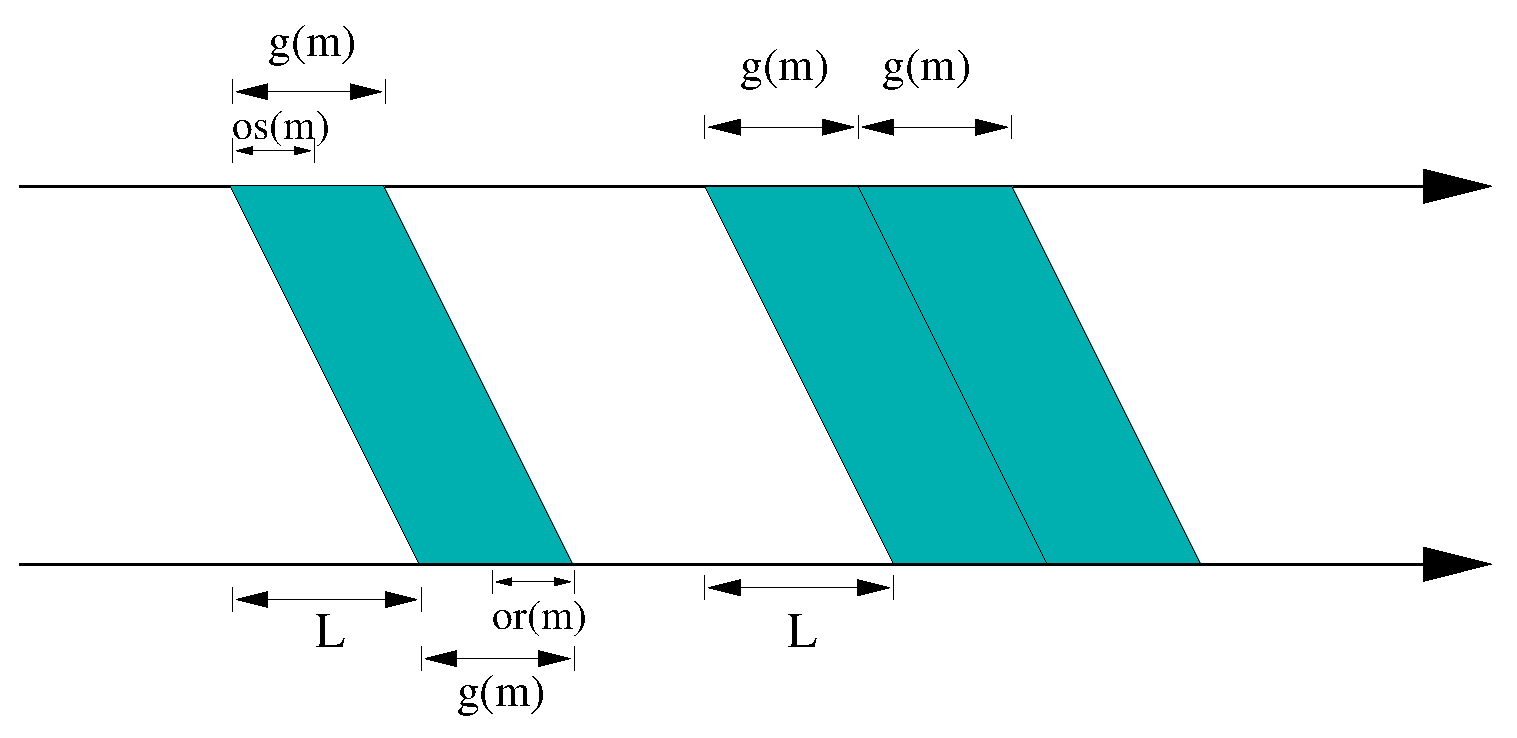
\includegraphics[width=0.7\linewidth]{images/p2p/plogp-struct}

\caption{\label{Figure: pLogP}Représentation d'une communication avec pLogP}

\end{figure}


En conséquence de cette nouvelle interprétation du \emph{gap}, les
paramètres $o_{s}$ et $o_{r}$ ont une importance moins évidente,
une fois que leur coût dans un réseau local est souvent recouvert
par celui du \textit{gap}.  Ainsi, pour représenter le temps nécessaire à la transmission d'un
message de taille \emph{m} entre deux n{\oe}uds avec des primitives de
communication bloquantes (i.e., où l'émetteur attend la fin de la transmission), le modèle pLogP utilise l'expression $L+g(m)$,
au lieu de $L+g+2o$ comme dans le modèle LogP. 


La variation des paramètres vis-à-vis de la taille des messages et des politiques d'émission est mise en évidence en Figure \ref{Figure: logp x hockney}, où on affiche les différents temps de communication mesurés avec la bibliothèque applicative LAM-MPI \cite{LAM04}. On observe un
changement de politique d'acquittement quand la taille des messages dépasse les 64 Ko, de manière à ce que le coût du \textit{gap} dépend à la fois
de la saturation de la fenêtre TCP et de la politique d'acquittement.

%
\begin{figure}
\centering
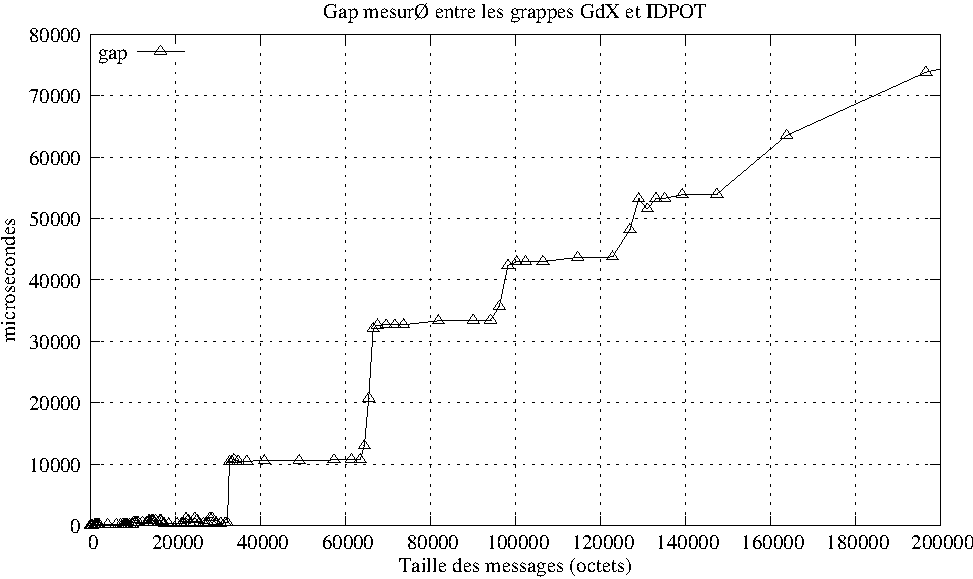
\includegraphics[width=0.7\linewidth]{images/p2p/hockney-logp1}

\caption{\label{Figure: logp x hockney}Valeurs de \textit{gap} mesurés entre deux machines
distantes \cite{Steffenel05c}}

\end{figure}



\section{Modélisation de l'Opération de Diffusion \textit{MPI\_Bcast}}

Parmi les opérations de communication collective, les diffusions de type \textit{Broadcast} sont parmi les plus simples et les plus répandues. Une opération de \emph{Broadcast} s'effectue quand un seul n{\oe}ud,
appelé \emph{racine,} envoie le même message de taille \emph{m} à
tous les autres $(P-1)$ n{\oe}uds.  Ceci représente en effet le patron de communication \textit{one-to-all}. 

Dans le cas du calcul distribué, la diffusion d'opérations est souvent nécessaire afin d'apporter des paramètres et des données à tous les n{\oe}uds.  La compréhension de ces mécanismes et la modélisation de ses coûts présente un intérêt stratégique vis-à-vis de la scalabilité et de l'optimisation des algorithmes. Dans ce sens, il est aussi nécessaire prendre en compte les différences architecturales des environnements de communication : les stratégies efficaces pour un environnement homogène diffèrent de celles adaptées aux environnements où les communications sont hétérogènes. Afin de représenter ces deux cas, nous nous sommes intéressés à la modélisation et l'optimisation des communications collectives de type \textit{Broadcast} dans deux types distincts de réseaux : les clusters (grappes de machines) et les \textit{grids} (grilles de calcul). Le premier cas  peut souvent être considéré comme homogène, alors que le deuxième apporte un degré d'hétérogénéité à cause des différences de communication intra et inter-cluster. Afin d'implémenter et valider des stratégies pour ces réseaux, nous avons choisi d'utiliser comme point de départ la bibliothèque MPI (Message Passing Interface), très utilisée par la communauté du calcul parallèle et qui dispose déjà d'une implémentation simple de l'opération \textit{broadcast} appelée MPI\_BCast.   

\subsection{\label{sec:Broadcast}Modélisation d'un \textit{Broadcast} dans un réseaux homogène}

L'opération \emph{Broadcast} est une des plus simples opérations de
communication collective : initialement, seul le n{\oe}ud \emph{racine}
détient le message qui doit être diffusé ; à la fin de l'opération,
une copie de ce message est déposée dans chaque n{\oe}ud du groupe.
L'approche classique pour implémenter l'opération \emph{Broadcast} utilise
des arbres qui sont décrits par deux paramètres, \emph{d} et \emph{h},
où \emph{d} est le nombre maximum de successeurs qu'un n{\oe}ud peut
avoir, et \emph{h} est la hauteur de cet arbre, le chemin le plus
long qui relie la racine et les feuilles de cet arbre. Plus généralement,
des arbres de diffusion avec différents degrés \emph{d} et \emph{h}
peuvent être générés à partir d'un algorithme de type \emph{arbre-alpha}
(\emph{alpha-tree} en anglais) suggéré par Bernaschi et Ianello \cite{Bernaschi98}.
À l'aide de cet algorithme et des paramètres du réseau, un arbre optimal
peut être construit à partir des paramètres du réseau et avec \emph{d,
	h $\in$}{[}1...\emph{P}-1] tel que $\sum_{i=o}^{h}d^{i}\geq P$ soit
respecté. %Cependant, pour une question de simplicité, la plupart des
%implémentations MPI utilisent des formes fixes telles que les arbres
%plats ou les arbres binomiaux. 

La performance des différentes formes fixes dépend surtout des paramètres
du réseau, notamment le \emph{gap}, la latence et le nombre de n{\oe}uds.
Par conséquent, un réseau avec une latence faible par rapport au \emph{gap}
favorise les algorithmes de type Arbre Binaire et Arbre Binomial,
qui cherchent à minimiser le temps de communication par la multiplication
des sources de transmission. Au contraire, si la latence est trop
élevée par rapport au \emph{gap}, les algorithmes de type Arbre Plat
sont favorisés, où un seul n{\oe}ud envoie des messages à tous les
autres. 


À partir des modèles de coût LogP \cite{Culler96} et pLogP \cite{Kielmann01}
et de travaux comme ceux de Huse \cite{Huse99}, Vadhiyar \cite{Vadhiyar00}
et autres, nous avons déduit les formules qui représentent différentes
stratégies de communication évaluées dans ce travail, comme indiqué
dans le Tableau \ref{table:bcast_models_classique}. Certaines de
ces stratégies sont clairement inefficaces, comme par exemple le \textit{broadcast}
en Chaîne, qui exécute $P-1$ communications en série. 

%
\begin{table}
	\centering
	\begin{tabular}{|c|c|}
		\hline 
		\textbf{\small Stratégie} & \textbf{\small Modèle de Communication}\tabularnewline
		\hline
		\hline 
		{\small Arbre Plat} & {\small $L+(P-1)\times g(m)$}\tabularnewline
		\hline 
		{\small Chaîne} & {\small $(P-1)\times(g(m)+L)$}\tabularnewline
		\hline 
		{\small Arbre Binaire} & {\small $\leq\lceil log_{2}P\rceil\times(2\times g(m)+L)$}\tabularnewline
		\hline 
		{\small Arbre Binomial} & {\small $\lceil log_{2}P\rceil\times L+\lfloor log_{2}P\rfloor\times g(m)$}\tabularnewline
		\hline
	\end{tabular}
	
	
	\caption{\label{table:bcast_models_classique}Modèles de communication pour
		le \emph{Broadcast}}
	
\end{table}


Une autre possibilité de construire un \emph{Broadcast} est la composition
des chaînes de retransmission \cite{Barnett96}. Cette stratégie,
possible grâce à la segmentation des messages, présente des avantages
importants, comme l'indiquent \cite{Kielmann01}\cite{Thakur03}\cite{Beaumont04a}.
Dans un \emph{Broadcast} Segmentée, la transmission des messages en
segments permet le recouvrement de la transmission d'un segment \emph{k}
et la réception du segment \emph{k}+1, minimisant le \emph{gap}.

Dans ce cas, nous considérons que le segment de taille \emph{s} d'un
message \emph{m} est un multiple de la taille du type basique de données
qui est transmis, divisant alors le message initial \emph{m} en \emph{k}
segments. Par conséquent, \emph{g(s)} représente le \emph{gap} d'un
segment de taille \emph{s}. Toutefois, le choix de la taille des segments
reste dépendant des caractéristiques du réseau. En effet, l'utilisation
de segments trop petits a un surcout non-négligeable dû à l'en-tête
du message, alors que l'utilisation des segments trop grands ne permet
pas l'exploitation intégrale du débit du réseau. 

La recherche de la taille de segment \emph{s} qui minimise le temps
de communication se fait à l'aide des modèles de communication présentés
dans le Tableau \ref{table:bcast_models_seg}. D'abord, on cherche
une taille de segment \emph{s} qui minimise le temps de communication
parmi $s=m/2^{i}\;\mathrm{pour}\; i\in[0\ldots log_{2}m]$. Ensuite,
on peut affiner la recherche de la taille optimale avec l'aide d'heuristiques
comme le "local hill-climbing" \cite{Kielmann01}.

%
\begin{table}
	\centering
	\begin{tabular}{|c|c|}
		\hline 
		\textbf{\small Stratégie} & \textbf{\small Modèle de Communication}\tabularnewline
		\hline
		\hline 
		{\small Arbre Plat Segmenté} & {\small $L+(P-1)\times(g(s)\times k)$}\tabularnewline
		\hline 
		{\small Chaîne Segmentée (Pipeline)} & {\small $(P-1)\times(g(s)+L)+(g(s)\times(k-1))$}\tabularnewline
		\hline 
		{\small Arbre Binomial Segmenté} & {\small $\lceil log_{2}P\rceil\times L+\lfloor log_{2}P\rfloor\times g(s)\times k$}\tabularnewline
		\hline
		{\small Pieuvre avec un degré }\emph{\small d} & {\small $(d+\lceil\frac{P-(2^{d}+1)}{(2^{d}+1)}\rceil)\times(g(s)+L)+(g(s)\times(k-1))$}\tabularnewline
		\hline
		{\small Scatter/Collection \cite{Thakur03}} & {\small $(log_{2}P+P-1)\times L+2\times(\frac{p-1}{p})\times g(m)$}\tabularnewline
		\hline
	\end{tabular}
	
	\caption{\label{table:bcast_models_seg}Modèles de communication segmentée
		pour le \emph{Broadcast}}
	
\end{table}


Pour valider ces modèles de communication, nous avons choisi la comparaison
entre les prédictions des modèles et les résultats réels obtenus à
partir d'expérimentations sur différentes plates-formes réseaux. Pour
illustrer notre approche, nous avons comparé des implémentations de
MPI\_Bcast selon les stratégies Arbre Plat, Arbre Binomial et Chaîne
Segmentée. Ainsi, les Figures \ref{Figure:Comparison-Bcast_Flat_FEth}
et \ref{Figure:Comparison-Bcast-Chain_FEth},
illustrent les valeurs mesurées expérimentalement des trois stratégies d'implémentation, qui suivent presque
fidèlement les prédictions des modèles.
%Dans les prochaines pages nous présentons l'analyse des
%expérimentations effectuées sur chaque plateforme réseau différente. 


%le réseau Fast Ethernet. 
\begin{figure}[h]
	\centering
	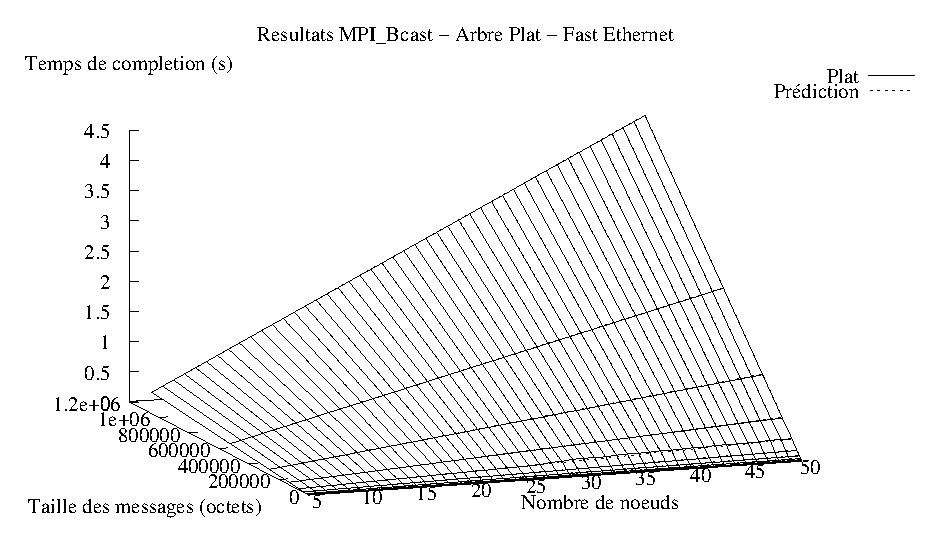
\includegraphics[width=0.5\linewidth]{images/modeles/FEth/Bcast/comp_Flat}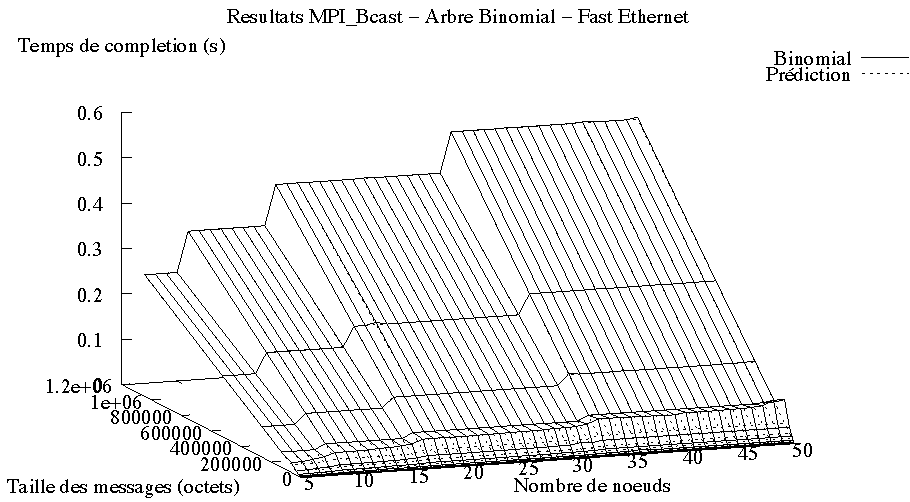
\includegraphics[width=0.5\linewidth]{images/modeles/FEth/Bcast/comp_Binomial}
	\caption{\label{Figure:Comparison-Bcast_Flat_FEth}Les performances réelles
		et prédites pour l'Arbre Plat (a) et l'Arbre Binomial (b) avec un réseau Fast Ethernet}
\end{figure}

%
\begin{figure}[h]
	\centering
	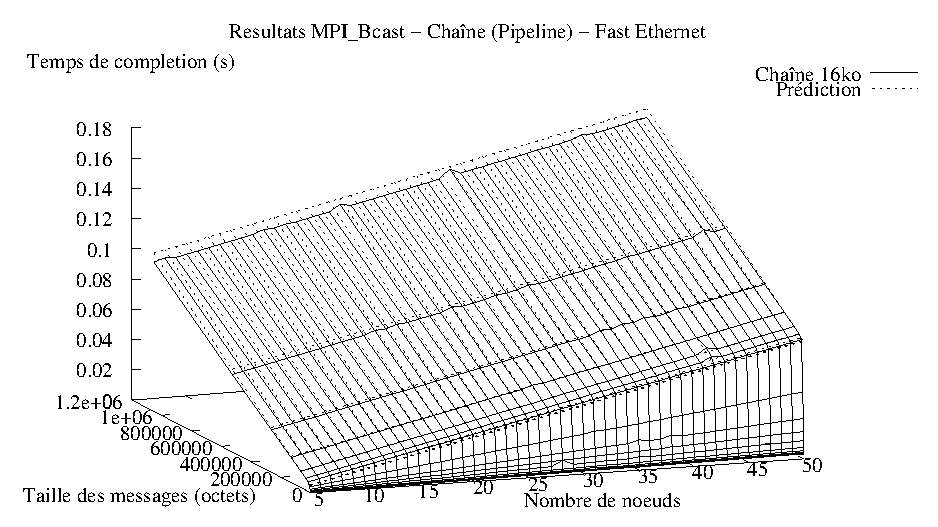
\includegraphics[width=0.5\linewidth]{images/modeles/FEth/Bcast/comp_Chain_16384}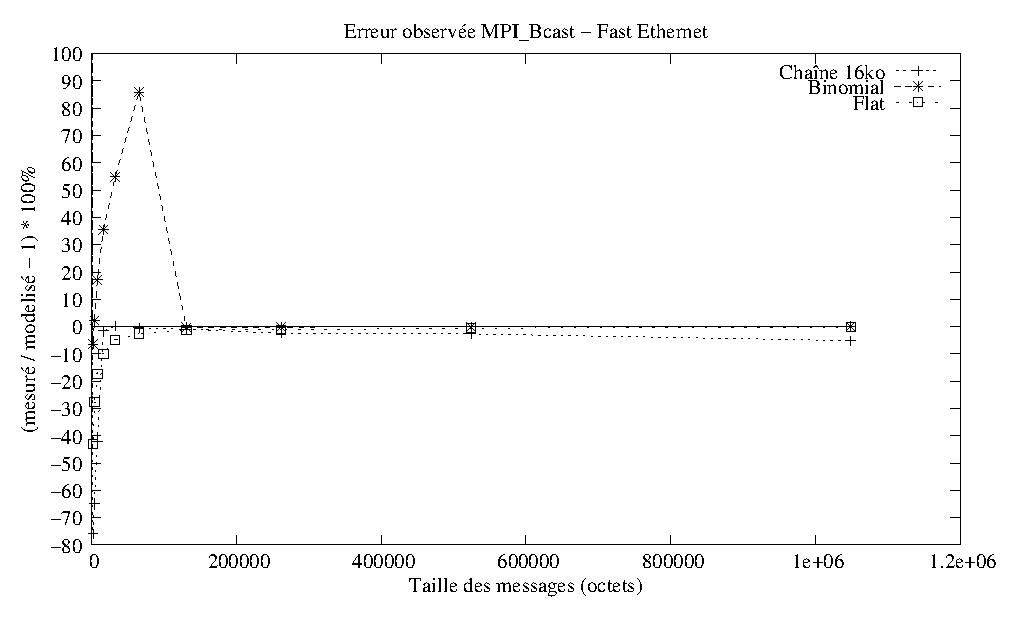
\includegraphics[width=0.5\linewidth]{images/modeles/FEth/Bcast/error}
	\caption{\label{Figure:Comparison-Bcast-Chain_FEth}Performances réelles
		et prédites pour la Chaîne Segmentée (a)  et l'erreur des prédictions par rapport
		aux valeurs mesurées (b)}
\end{figure}

Plus spécifiquement, des différences entre les prédictions et les
valeurs réelles sont observées surtout dans le cas de l'envoi de petits messages, qui ne suit pas un comportement linéaire
par rapport à la taille des messages. Cette variation de performance
a été l'objet d'analyses précédentes (cette discussion peut être retrouvée
dans les articles \cite{Steffenel04a} et \cite{Steffenel04c}) et doit son origine à l'implémentation des politiques de 
transmission et d'acquittement TCP, qui parfois opte pour retarder l'envoi de petits messages. 

En effet, TCP dispose d'une option \emph{socket} TCP\_NODELAY qui devrait permettre l'envoi de tout message sans attente. 
Seulement, nous avons observé que parfois un seul message
à chaque \emph{n} messages transmis n'est pas acquitté comme il le
faut. Cette défaillance de l'implémentation protocole d'acquittement induit un temps supplémentaire
 qui se reflète sur un surcout lors de l'envoi de petits messages.  


La Figure \ref{Figure:Comparison-Bcast-Chain_FEth} résume aussi ces trois stratégies en affichant le taux d'erreur entre les mesures et les prédictions.
Ici, nous observons que les résultats réels, normalement très proches
des prédictions (à une marge de 10\% maximum), s'écartent des prédictions
jusqu'à 90\% pour des messages autour de 128 Ko. Néanmoins, ces variations
affectent des communications où la différence absolue n'est que de
quelques millisecondes, ce qui n'empêche pas l'utilisation des modèles
de communication pour choisir la meilleure stratégie de communication. 


\subsection{Modélisation du \textit{Broadcast} dans un \textit{Grid}}

La détermination du meilleur arbre de diffusion pour un environnement
homogène est une tâche relativement facile car dépend de paramètres de latence et débit ( ou par extension, du \textit{gap}) communs à tout le réseau.  

Cependant, dans le cas d'un réseau hétérogène, ce problème devient
bien plus difficile à cause des variations des paramètres de communication entre chaque pair de n{\oe}uds. En effet, l'identification du meilleur arbre
de diffusion dans un réseau hétérogène est un problème NP-complet \cite{Bhat99}\cite{Beaumont04c,Beaumont05b}\cite{PangfengLiu04}.
La plupart des travaux dédiés à l'optimisation des communications
collectives dans des environnements hétérogènes essayent donc de construire des arbres de diffusion en tenant compte du coût d'interconnexion entre chaque pair de n{\oe}ud concernée par le \textit{broadcast}. C'est le cas de Banikazemi \cite{Banikazemi98},
Bhat \cite{Bhat99,Bhat03} ou Mateescu \cite{Mateescu05}.

Cependant, l'environnement de type \textit{grid} est normalement caractérisé
par un grand nombre de n{\oe}uds communicants, résultat de l'association
des différents \textit{clusters}. Dans ce cas, la complexité de la
tâche d'optimisation est bien plus importante, et des simplifications
s'imposent afin de permettre l'utilisation de telles méthodes dans
la pratique. Une de ces simplifications est le regroupement des n{\oe}uds
selon leurs performances relatives (par exemple, par rapport à la
communication), de manière à ce que toute une classe de n{\oe}uds
puisse être traitée comme une entité unique. De cette manière, le nombre important de n{\oe}uds dans un \textit{grid} peut être
encore facilement abordable par les méthodes d'optimisation classiques grâce à la division des communications en deux catégories, l'\textit{inter-cluster} et l'\textit{intra-cluster}. 


Cependant, à défaut de leur apport aux algorithmes de \textit{Broadcast}, ces
techniques peuvent encore être améliorées. En effet, les travaux précédents
ont été établis dans un contexte où les communications de longue distance
étaient plusieurs ordres plus lentes que celles à l'intérieur des
réseaux locaux, et la réduction des communications \textit{inter-clusters} permettait
la minimisation de la congestion sur les liens les plus lents. Si
cela est encore vrai en ce qui concerne la latence entre les n{\oe}uds,
il n'est plus exact pour le débit d'un lien de longue distance. D'autre
part, le faible coût du matériel informatique permet aujourd'hui que
les  \textit{clusters} regroupent des centaines de n{\oe}uds. Or, plus le coût de
diffusion \textit{intra-clusters} devient important, plus son influence
sur la performance sera importante au moment de définir l'ordonnancement
des communications.

C'est exactement ce qui différencie les heuristiques traitant (ou
ne traitant pas) la communication à l'intérieur des groupes : les
heuristiques "traditionnelles" et celle appelées "heuristiques
sensibles au contexte des \textit{grids}" ("\emph{grid-aware}"
en anglais). Dans le premier cas, l'optimisation ne tient compte que
des communications entre les différents coordinateurs, alors que le
deuxième cas s'occupe aussi de la diffusion à l'intérieur des  \textit{clusters}. 


Les prochaines sections présentent les différentes heuristiques étudiées
pour l'optimisation des communications de type MPI\_Bcast. Certaines
de ces heuristiques sont la simple application des méthodes pour les
réseaux hétérogènes dans le contexte des  \textit{clusters} hiérarchisées. Dans
ce travail nous proposons trois nouvelles méthodes, qui au contraire
des techniques précédentes, considèrent autant les communications
entre les coordinateurs que les temps nécessaires à la diffusion des
messages à l'intérieur des  \textit{clusters}.


\subsubsection*{Formalisme utilisé}

Pour décrire les heuristiques présentées dans cette section, nous
utilisons un formalisme de groupes similaire à celui de Bhat \cite{Bhat03}.
Dans ce formalisme, les  \textit{clusters} sont séparés en deux groupes, \textbf{A}
et \textbf{B}. Le groupe \textbf{A} contient les  \textit{clusters} qui ont déjà
reçu le message (la réception du message par le coordinateur du
 \textit{cluster} est suffisante). Le groupe \textbf{B} contient les  \textit{clusters}
qui devront recevoir le message. De cette manière, le groupe \textbf{A}
contient initialement le  \textit{cluster} du n{\oe}ud \emph{source} ou \emph{racine},
tandis que le groupe \textbf{B} contient toutes les autres  \textit{clusters}
du réseau.

À chaque étape, un émetteur appartenant au groupe \textbf{A} et un
récepteur appartenant au groupe \textbf{B} sont choisis. Après la
communication entre ces deux  \textit{clusters} (plus exactement, leurs coordinateurs),
le \textit{cluster} récepteur est transféré au groupe \textbf{A}. 

L'implémentation de ces communications est faite de manière à rendre
prioritaires les communications entre les  \textit{clusters}. En effet, les coordinateurs
diffusent le message à l'intérieur de ses  \textit{clusters} seulement après
la fin des communications \textit{inter-clusters}. Cette stratégie favorise
la multiplication des sources disponibles et l'application des heuristiques,
ainsi que la prédiction du temps total d'exécution du \textit{Broadcast}.

\subsection*{Heuristiques Traditionnelles}

\subsubsection*{Diffusion en Arbre Plat (Flat)}

L'heuristique en \emph{Arbre Plat}, découpe la communication en deux niveaux, \emph{inter-clusters}
et \emph{intra-clusters}. 

Dans le premier niveau, le n{\oe}ud \emph{racine} envoie le message
à tous les coordinateurs des différents \textit{clusters}. L'ordre d'envoi
suit le "rang" des différents \textit{clusters}, prédéfini à l'initialisation.
Formellement, cela veut dire qu'à chaque étape, le n{\oe}ud \emph{racine}
choisi comme récepteur le premier  \textit{cluster} du groupe \textbf{B}. Dans
cette "heuristique", le n{\oe}ud émetteur est toujours
le même (le n{\oe}ud \emph{racine}), malgré le fait que les  \textit{clusters}
qui ont déjà reçu le message font désormais partie du groupe \textbf{A}.
Dans le deuxième niveau de diffusion, exécuté à l'intérieur de chaque
 \textit{cluster}, les coordinateurs exécutent un \emph{broadcast} en arbre binomial.

Même si cette heuristique est très simple à implémenter, elle est toutefois
très peu optimisée. En effet, la diffusion des données ne tient pas
compte des performances des différents  \textit{clusters}, ni les vitesses d'interconnexion
entre les \emph{coordinateurs}. Même si l'utilisateur organise le
fichier de description des  \textit{clusters} de manière à favoriser les communications
émises d'un certain  \textit{cluster}, celles-ci restent soumises à une structure
de diffusion \emph{plate}. 


\subsubsection*{Fastest Node First - FNF}

L'heuristique \emph{Fastest Node First} (le n{\oe}ud le plus rapide d'abord)
a été proposée par Banikazemi \emph{et al.} \cite{Banikazemi98}.
Dans leur modèle de communication, le réseau est composé d'un certain
nombre de n{\oe}uds \emph{$P$}. À chaque n{\oe}ud \emph{$P_{\textrm{i}}$}
on associe un coût d'envoi \emph{$C_{\textrm{i}}$}. Ce coût \emph{$C_{\textrm{i}}$}
est indépendant de la destination et de la taille du message, et indique
seulement la différence de vitesse entre les n{\oe}uds.

L'heuristique proposée par Banikazemi \emph{et al.} nécessite $P-1$
itérations, où à chaque étape l'heuristique définie un émetteur et
un récepteur. Le récepteur est choisi parmi les possibles récepteurs
du groupe \textbf{B} dont le coût \emph{$C_{\textrm{i}}$} est le
plus petit. L'émetteur est le n{\oe}ud du groupe \textbf{A} qui peut
finir la communication le plus rapidement possible. Cela dit, cette
stratégie choisit l'émetteur le plus rapide et le récepteur qui pourrait
retransmettre les messages le plus rapidement possible, à son tour.

L'efficacité de l'heuristique FNF dans le cadre des environnements
homogènes a été démontrée par Liu \cite{PangfengLiu00b}, qui a prouvé que
l'heuristique FNF produit des ordonnancements avec au plus deux fois
le temps optimal.

Cependant, des environnements homogènes comme ceux considérés par
Banikazemi sont assez rares dans les \textit{grids}, ce qui rend cette heuristique
très limitée par rapport à la modélisation des communications. En
effet, le modèle de coût unique $C_{\textrm{i}}$ n'est pas suffisant
pour représenter l'hétérogénéité d'un réseau d'interconnexion, comme
indiqué par Bhat \cite{Bhat03}. 


\subsubsection*{Fastest Edge First - FEF}

Proposée par Bhat \emph{et al.} \cite{Bhat03}, l'heuristique \emph{Fastest
	Edge First} (l'arête la plus rapide d'abord) est un algorithme glouton
qui fait partie d'une collection d'heuristiques proposées comme alternative
à l'heuristique FNF. 

Assez simple, cette heuristique est très similaire à l'heuristique
FNF. Seulement, au lieu d'un coût de communication unique $C_{\textrm{i}}$,
l'heuristique évalue le poids de chaque lien de communication $L_{i,j}$
entre deux n{\oe}uds différents (les arêtes), correspondants à la latence
de communication entre les deux n{\oe}uds. 

Pour identifier l'ordonnancement des communications nécessaire à l'exécution
de l'opération de \textit{Broadcast}, l'algorithme FEF, ordonne les n{\oe}uds
du groupe A selon leurs arêtes les plus rapides. Cela permet le choix
du lien le plus rapide parmi toutes les possibilités, et en même temps,
sert à définir l'émetteur et le récepteur, déterminés implicitement
par l'arête choisie. Une fois que le récepteur est désigné, celui-ci
est transféré du groupe \textbf{B} vers le groupe \textbf{A}. À cet
instant, les arêtes minimales doivent être recalculées.

Le raisonnement de cette heuristique est que le choix des liens les
plus rapides permet d'augmenter rapidement le nombre d'émetteurs.
À leur tour, ces émetteurs pourront disséminer le message vers les
n{\oe}uds les plus éloignés, tout en choisissant le lien le moins
coûteux.


\subsubsection*{Early Completion Edge First - ECEF}

Selon les heuristiques précédentes, une fois que le récepteur était
assigné, celui-ci était immédiatement transféré vers le groupe des
émetteurs, le groupe \textbf{A}. Toutefois, à cause des délais de
communication, il est possible que ce récepteur n'ait pas encore reçu
le message et qu'il soit choisi pour le retransmettre à un deuxième
n{\oe}ud. La communication subira un retard supplémentaire, alors
qu'une autre arête, moins rapide, pourrait finir la transmission plus
vite si son émetteur a déjà le message. 

Pour tenir compte des retards dus à la transmission des données, l'heuristique
\emph{Early Completion Edge First} (arête qui finit le plus tôt) considère
aussi dans son évaluation l'instant où les émetteurs ont les données
disponibles pour l'envoi. Ainsi, la \emph{disponibilité} $RT_{i}$
du n{\oe}ud émetteur (\emph{Ready Time} en anglais) est alors utilisée
conjointement avec le temps nécessaire à la transmission du message
entre les n{\oe}uds (le \textit{gap} plus la latence) de manière à choisir
le couple émetteur-récepteur qui minimise le temps : 

\[
RT_{i}+g_{i,j}(m)+L_{i,j}\]


Ainsi, l'objectif de cette heuristique est d'augmenter le nombre de
n{\oe}uds qui peuvent \emph{effectivement} transmettre les messages
aux autres n{\oe}uds.


\subsubsection*{Early Completion Edge First with lookahead - ECEF-LA}

Pour augmenter l'efficacité de l'heuristique précédente, la dernière
heuristique proposée par Bhat \emph{et al.} \cite{Bhat03} propose
une recherche plus approfondie sur les possibles choix. En effet,
si l'objectif des heuristiques précédentes était la multiplication
des sources disponibles, cela suppose que ces sources pourront, à
leur tour, retransmettre les messages de manière efficace.

C'est ainsi que Bhat a proposé l'utilisation d'une fonction de \emph{lookahead}
(recherche en avant) pour évaluer si le choix d'un récepteur est réellement
bon. De cette manière, l'algorithme calcule préalablement la fonction
de \emph{lookahead} $F_{j}$ pour tous les n{\oe}uds dans le groupe
\textbf{B}, et la pair émetteur-récepteur est celle qui minimise
la somme :

\[
RT_{i}+g_{i,j}(m)+L_{i,j}+F_{j}\]


Cette fonction de \emph{lookahead} peut être définie de plusieurs
façons. Bhat \cite{Bhat03} propose, par exemple, le coût minimal
pour que le n{\oe}ud \emph{j} transmette à d'autres n{\oe}uds encore
dans le groupe \textbf{B}. Cette fonction est alors la suivante :

\begin{eqnarray*}
	F_{j} & = & \min_{P_{k}\in B}\,(g_{j,k}(m)+L_{j,k})\end{eqnarray*}


Intuitivement, cette fonction indique l'utilité du n{\oe}ud $P_{j}$
si à son tour il est transféré vers le groupe \textbf{A}. D'ailleurs,
Bhat a proposé d'autres fonctions de \emph{lookahead}, dont par exemple
la moyenne de la latence entre $P_{j}$ et les autres n{\oe}uds en
\textbf{B}, ou alors la latence moyenne entre les émetteurs et les
récepteurs, si on considère que $P_{j}$ est transféré vers le groupe
\textbf{A}. 


\subsection*{Heuristiques "grid-aware"}

Les heuristiques présentées précédemment hiérarchisent les communications en deux niveaux - \emph{inter-clusters}
et \emph{intra-clusters}, mais les fonctions d'évaluation ne tiennent compte que des coûts de transmission entre les coordinateurs
des différentes  \textit{clusters} du réseau.

Comme nous l'avons déjà exposé, le coût d'une communication
hiérarchique ne dépend pas seulement des latences entre les différentes
 \textit{clusters}, mais aussi du temps nécessaire à la diffusion des messages
à l'intérieur de ces  \textit{clusters}. Ce coût de diffusion \textit{intra-clusters} devient
encore plus important avec l'augmentation du nombre de n{\oe}uds à l'intérieur
des  \textit{clusters}, qui aujourd'hui dépasse facilement la centaine de machines.
Par exemple, l'envoi d'un message de 1Mo entre deux \textit{clusters} (l'un à Grenoble, l'autre à Paris) requiert 349 millisecondes, alors que
le \textit{broadcast} de ce même message entre 50 n{\oe}uds du \textit{cluster} de Grenoble
peut nécessiter jusqu'à 3 secondes selon l'algorithme
utilisé. Si ce temps n'est pas pris en compte lors de la modélisation
des communications, l'ordonnancement des communications risque d'être
sous-optimal.

Plus exactement, le temps de diffusion \textit{intra-clusters}, appelé $T_{k}$,
correspond aux prédictions des modèles de communication vus précédemment. 
Cette notation $T_{k}$ est équivalente à une notation où un n{\oe}ud
fictif $k'$ est associé à chaque coordinateur $k$, dont :

\[
L_{k,k'}+g_{k,k'}=\left\{ \begin{array}{c}
\begin{array}{cc}
T_{k} & si\: k'\, est\, associe\, a\, k\\
\infty & \,\,\,\,\,\,\,\,\,\,\,\,\, pour\, tout\, autre\, noeud\, j\neq k\end{array}\end{array}\right.\]


La présence d'un n{\oe}ud fictif permet l'utilisation des heuristiques
précédentes sans la nécessité d'une modification des algorithmes,
notamment le ECEF. L'utilisation de $T_{k}$ permet une implémentation
plus simple des algorithmes, qui n'ont pas besoin de garder les deux
identités \emph{k} et \emph{k'} associées à un  \textit{cluster} \emph{k}. Toutefois, dans ce travail nous avons gardé
la description séparée \emph{L}, \emph{g} et \emph{T}, afin
de permettre une identification plus facile des facteurs évalués.

Dans ce sens, nous présentons deux nouvelles stratégies d'évaluation
dites "sensibles au contexte des \textit{grids}", où
le temps de diffusion \emph{intra-cluster} est aussi considéré lors
de la construction des arbres de diffusion. Pour mieux analyser l'efficacité
de ces stratégies, nous avons aussi développé une version de l'heuristique
ECEF-LA où le temps \textit{intra-clusters} est pris en compte. Cette version
sert de comparaison par rapport aux heuristiques de Bhat, présentées
précédemment. 


\subsubsection*{ECEF-LA\emph{t}}

L'heuristique ECEF-LA\emph{t} est l'évolution naturelle de l'heuristique
ECEF-LA où nous utilisons une fonction de \emph{lookahead} adaptée
à la représentation du coût de communication \textit{intra-clusters} $T_{k}$. 

Ainsi, l'heuristique ECEF-LA\emph{t} cherche à minimiser le coût total
de transmission et le temps nécessaire à la diffusion d'un message
dans un  \textit{cluster} distant (en effet, le "petit \emph{t}"
du nom de cette heuristique indique qu'on cherche le minimum des temps).
Pour cela, elle utilise une fonction d'évaluation :

\begin{eqnarray*}
	F_{j} & = & \min_{P_{k}\in B}\,(g_{j,k}(m)+L_{j,k}+T_{k})\end{eqnarray*}


À l'instar de l'heuristique ECEF-LA, le but de cette stratégie est
que le récepteur soit choisi parmi les  \textit{clusters} qui peuvent retransmettre
le message le plus vite possible à d'autres  \textit{clusters}. L'adjonction
du temps $T_{k}$ dans la fonction d'évaluation implique aussi que
le choix d'un interlocuteur minimisera le temps de complétion des
 \textit{clusters} contactés dans le futur. 


\subsubsection*{ECEF-LA\emph{T}}

Une contrepartie de la technique précédente est que cette stratégie
a tendance à favoriser les  \textit{clusters} rapides, ce qui peut entraîner
des retards supplémentaires aux  \textit{clusters} plus lents, reléguées aux
dernières places. Pour éviter une telle situation, nous proposons
une nouvelle fonction de \emph{lookahead}, où le choix des  \textit{clusters}
considère le maximum du temps nécessaire à la transmission et à la
diffusion d'un message : 

\begin{eqnarray*}
	F_{j} & = & \max_{P_{k}\in B}\,(g_{j,k}(m)+L_{j,k}+T_{k})\end{eqnarray*}


Malgré sa similarité avec l'heuristique précédente, cette nouvelle
fonction d'évaluation cherche à équilibrer le temps de communication
vers les différents  \textit{clusters}, lentes ou rapides. En effet, nous cherchons
dans un premier instant le  \textit{cluster} la plus lente qu'il reste à contacter
(la fonction de \emph{lookahead}), et parmi les choix d'émetteurs
disponibles, nous choisissons celui qui peut la contacter le plus
rapidement possible (fonction d'évaluation \emph{min} de l'heuristique
ECEF).

Le raisonnement de cette heuristique est que si les  \textit{clusters} les plus
distants ou les plus lents (dans le sens où la diffusion des messages
prend plus de temps) sont contactés en dernière place, leur diffusion
prendra encore plus de retard, ce qui augmentera le temps d'exécution
du \textit{Broadcast}. Avec la fonction de \emph{lookahead} de ECEF-LA\emph{T},
nous choisissons comme récepteur le  \textit{cluster} qui prendra le moins de
temps possible pour contacter le  \textit{cluster} le plus lent : cela garantit
que si besoin est, les  \textit{clusters} les plus lents seront contactés dans
le minimum de temps possible.


\subsubsection*{BottomUp}

La troisième heuristique proposée dans ce travail utilise une logique
d'optimisation différente de celle utilisée par Bhat. En effet, l'approche
de Bhat vise toujours la minimisation des facteurs liés à la transmission
des messages et à sa diffusion, ce qui généralement finit par donner
priorité aux  \textit{clusters} les plus rapides. Cependant, nous considérons
que le temps d'exécution d'un \textit{Broadcast} hiérarchique dépend surtout
des  \textit{clusters} les plus lents.

À partir des heuristiques précédentes, nous observons que, malgré
l'utilisation de différentes fonctions de \emph{lookahead}, les heuristiques
de type ECEF-LA suivent toujours l'approche \emph{min-max} ou \emph{min-min}.
Or, l'heuristique ECEF-LA\emph{T} considère que parfois il est plus
intéressant d'envoyer les messages d'abord aux  \textit{clusters} les plus lents,
pour ne pas retarder encore plus leur diffusion. D'autre part, il
est aussi vrai qu'un grand nombre d'émetteurs favorise la conclusion
rapide du \textit{Broadcast}, et que l'envoi à des  \textit{clusters} plus lents n'aide
guère à augmenter le nombre d'émetteurs. Si ces deux raisonnements
sont a priori opposés, ils ne sont pas incompatibles. En effet, les
deux approches peuvent être combinées si des règles précises sont
déterminées.

C'est ainsi que dans l'heuristique \textit{BottomUp} nous définissons initialement
une approche de type \emph{max-min}, où l'émetteur est choisi parmi
les  \textit{clusters} qui pourront contacter le plus rapidement possible le
 \textit{cluster} le plus lent du réseau :

\[
\max_{P_{j}\in B}\,(\min_{P_{i}\in A}\,(g_{i,j}(m)+L_{i,j}+T_{j}))\]


En effet, cette approche permet que les  \textit{clusters} les plus lents soient
contactés dans le plus petit temps possible, ce qui peut minimiser
le retard imputé à ces  \textit{clusters}. Toutefois, cette technique n'offre
aucune garantie sur l'efficacité future des  \textit{clusters} émetteurs. Pour
cela, il serait peut-être intéressant d'ajouter une fonction de \emph{lookahead},
à l'exemple des heuristiques de type ECEF-LA.


\subsection{Évaluation pratique}

Les différentes heuristiques ont été implémentées sur une version modifiée
de la bibliothèque MagPIe\cite{Kielmann99b}, que nous avons adapté pour l'acquisition
et la manipulation des paramètres de communication entre les  \textit{clusters}. Cette procédure de
découverte de topologie permet non seulement le regroupement des n{\oe}uds
en \textit{clusters} logiques homogènes (plus adaptées à la modélisation de
performance), mais aussi fait automatiquement l'acquisition des paramètres
pLogP correspondant à chaque sous-réseau homogène. Ces paramètres
pLogP, une fois chargés en mémoire, sont associés à la structure hiérarchique
du réseau. Ils sont utilisés pour prédire la performance des communications et pour choisir les meilleures
stratégies selon les caractéristiques des réseaux.

Pour cette validation nous avons utilisé 88 machines réparties entre les \textit{clusters}
d'Orsay, Toulouse et Grenoble. Nous avons utilisé 60 machines
du  \textit{cluster} d'Orsay, 20 machines du  \textit{cluster} de Toulouse et
8 machines du  \textit{cluster} de Grenoble. Après la découverte de la topologie du réseau, ces machines ont été regroupées en 6
\textit{clusters} homogènes différentes comme indiqué par le Tableau \ref{Tableau: Latence grid 1}. 

\begin{table}
	\caption{\label{Tableau: Latence grid 1}Latence entre les différents \textit{clusters}
		(en microsecondes)}
	
	
	\begin{centering}
		{\footnotesize }\begin{tabular}{|c||c|c|c|c|c|c|}
			\hline 
			& {\footnotesize  Cluster 0} & {\footnotesize  Cluster 1} & {\footnotesize  Cluster 2} & {\footnotesize Cluster 3} & {\footnotesize  Cluster 4} & {\footnotesize  Cluster 5}\tabularnewline
			\hline 
			& {\footnotesize 31 x Orsay} & {\footnotesize 29 x Orsay} & {\footnotesize 6 x IDPOT} & {\footnotesize 1 x IDPOT} & {\footnotesize 1 x IDPOT} & {\footnotesize 20 x Toulouse}\tabularnewline
			\hline
			\hline 
			{\footnotesize  Cluster 0} & {\footnotesize 47.56} & {\footnotesize 62.10} & {\footnotesize 12181.52} & {\footnotesize 12187.24} & {\footnotesize 12197.49} & {\footnotesize 5210.99}\tabularnewline
			\hline 
			{\footnotesize  Cluster 1} & {\footnotesize 62.10} & {\footnotesize 47.92} & {\footnotesize 12181.52} & {\footnotesize 12198.03} & {\footnotesize 12195.22} & {\footnotesize 5211.47}\tabularnewline
			\hline 
			{\footnotesize  Cluster 2} & {\footnotesize 12181.52} & {\footnotesize 12181.52} & {\footnotesize 35.52} & {\footnotesize 60.08} & {\footnotesize 60.08} & {\footnotesize 5388.49}\tabularnewline
			\hline 
			{\footnotesize  Cluster 3} & {\footnotesize 12187.24} & {\footnotesize 12198.03} & {\footnotesize 60.08} & {\footnotesize 0$^{*}$} & {\footnotesize 242.47} & {\footnotesize 5393.98}\tabularnewline
			\hline 
			{\footnotesize  Cluster 4} & {\footnotesize 12197.49} & {\footnotesize 12195.22} & {\footnotesize 60.08} & {\footnotesize 242.47} & {\footnotesize 0$^{*}$} & {\footnotesize 5394.10}\tabularnewline
			\hline 
			{\footnotesize  Cluster 5} & {\footnotesize 5210.99} & {\footnotesize 5211.47} & {\footnotesize 5388.49} & {\footnotesize 5393.98} & {\footnotesize 5394.10} & {\footnotesize 27.53}\tabularnewline
			\hline
		\end{tabular}
		\par\end{centering}{\footnotesize \par}
	
	\begin{centering}
		{\footnotesize {*} ce \textit{cluster} contient une seule machine.}
		\par\end{centering}
\end{table}


La Figure \ref{Figure: Bcast - Case1 - Mesure} présente ainsi les temps de communication de chacune de ces stratégies. Le premier résultat à noter est la faible performance de la stratégie
\textit{Flat}, même par rapport à l'implémentation par défaut de MPI. Cela
ne veut pas dire que la stratégie \textit{Flat} est toujours moins performante
que les autres stratégies, mais indique que cette stratégie est trop
dépendante de la configuration du réseau, de l'ordre de représentation
des \textit{clusters} et du n{\oe}ud racine.
%
\begin{figure}[h]
	\centering
		\includegraphics[width=0.7\linewidth]{images/Grid/Bcast/case1/comp}
	\caption{\label{Figure: Bcast - Case1 - Mesure}Performance du \textit{Broadcast} sur
		un \textit{grid} de 88 machines }	
\end{figure}

\begin{figure}[h]
	\centering
		\includegraphics[width=0.7\linewidth]{images/Grid/Bcast/case1/simul}	
	\caption{\label{Figure: Bcastcase1predictions}Prédictions pour un \textit{grid}
		avec 88 machines}
	
\end{figure}

Dans le cas des autres heuristiques, on observe des gains de performance
déjà très importants. L'heuristique \textit{BottomUp} %, comme prévu par lessimulations, 
n'est pas aussi efficace que les autres heuristiques,
qui de leur côté, se comportent de manière très similaire.

Le faible écart observé entre les prédictions des heuristiques de
type FEF et ECEF-{*} est justifié surtout par le nombre réduit de
\textit{clusters}, qui réduit le nombre de combinaisons possibles et fait converger
les résultats des différentes heuristiques. 

Pour mieux valider les résultats des expériences, la Figure \ref{Figure: Bcastcase1predictions}
présente les temps prévus des différentes heuristiques. Ces temps,
calculés automatiquement par les heuristiques d'ordonnancement des
communications, donnent une meilleure indication de la fiabilité des
modèles par rapport aux résultats pratiques. Dans ce cas, nous observons
que les heuristiques de type FEF et ECEF-{*} ont des résultats très
rapprochés, certainement parce qu'elles ont obtenu le même ordonnancement
des communications. D'un autre côté, l'écart entre ces prédictions
et les résultats réels sont bien plus importants pour les heuristiques
FEF et ECEF-{*} que pour le \textit{BottomUp} ou le \textit{Flat}. Cela indique que
le coût du calcul de l'ordonnancement et le coût de la mise en {\oe}uvre
de ces communications sont les facteurs les plus importants, et reflètent
l'augmentation de complexité d'une communication à couches multiples.

Cette étude met en évidence l'importance
du n{\oe}ud racine et de la répartition des n{\oe}uds sur des différents
\textit{clusters} sur la performance des stratégies plus simples. En effet,
la performance de la stratégie \textit{Flat} est fortement liée à l'ordre des \textit{clusters}, généralement fournie par l'utilisateur.
De surcroît, la stratégie \textit{Flat} utilise toujours le même ordre de diffusion,
indépendamment du rang du n{\oe}ud racine. Au contraire, les heuristiques
les plus élaborées construisent des arbres de diffusion adaptés à
chaque situation, ce qui rend possible un gain de performance plus
important, surtout quand le rôle de \emph{racine} est alterné entre
plusieurs n{\oe}uds.

D'ailleurs, les simulations indiquent que la performance des stratégies
simples, comme le \textit{Flat}, supportent très mal l'augmentation du nombre
de \textit{clusters} interconnectés.  Ainsi, nous croyons que, même si
le \textit{grid} compte un nombre réduit de \textit{clusters}, l'utilisation d'une
heuristique un peu plus élaborée, comme par exemple l'heuristique
ECEFLA-T, offre le meilleur rapport coût-bénéfice-robustesse.


\section{Amélioration de la Performance de MPI\_AlltoAll \\dans un \textit{Grid}}

Si les stratégies présentées dans les sections précédentes permettent l'optimisation des communications dans le cadre d'une diffusion MPI\_Bcast, d'autres patrons de communication encore plus couteux sont utilisés par les applications scientifiques. L'une de ces patrons, le \textit{many-to-many}, représente un \emph{échange total} d'informations entre les n{\oe}uds \cite{Christara99}. Plus exactement, chaque n{\oe}ud détient $n$ items de données différentes de taille $m$, lesquels doivent être distribués entre $n$ n{\oe}uds (le n{\oe}ud inclus).  

Vu la complexité de l'opération, les implémentations de \textit{many-to-many} dans la bibliothèque MPI (appelées "\textit{All-to-All}" par celle-ci) généralement utilisent des envois directs entre les n{\oe}uds, ce qui peut occasionner la surcharge des communications et des problèmes liés à la congestion du réseau. De surcroît, l'utilisation de cette approche dans un environnement de type grille doit aussi faire face à l'hétérogénéité des temps de communication entre les n{\oe}uds proches et distants.

\subsection{Définitions}

Soit deux \textit{clusters} ${\mathcal C}_1$
et ${\mathcal C}_2$ avec respectivement $n_1$ n{\oe}uds et $n_2$ n{\oe}uds.
Un réseau, appelé \textit{backbone}, interconnecte les deux \textit{clusters}. Nous assumons aussi que l'interface réseau utilisée pour la communication avec un réseau distant est la même utilisée pour la communication avec le réseau local. De ce fait et de la topologie du réseau, les communications \textit{inter-cluster} ne seront jamais plus rapides que celles effectuées à l'intérieur d'un \textit{cluster}.

Maintenant supposons qu'une application doit échanger des données entre les machines dans ${\mathcal C}_1$ et ${\mathcal C}_2$ et que pour chaque source, les données à destination des autres machines ne sont pas identiques (mais ont toutes une taille $m$).  Comme résultat, nous devons transmettre l'équivalent à $(n_1+ n_2)^2$ messages différents. Alors que plusieurs bibliothèques MPI  (OpenMPI, MPICH2, etc.) implémentent l'opération \textit{MPI\_AllltoAll} en supposant que les n{\oe}uds se trouvent dans le même réseau et donc que les communications ont le même coût, dans notre cas certains messages sont envoyés entre n{\oe}uds d'un même \textit{cluster} et d'autres entre n{\oe}uds de réseaux différents. Dans le premier cas, la latence des communications est plus favorable que dans le deuxième, et souvent le même principe s'applique pour le débit du réseau.


\subsection{Modélisation de la Congestion du Réseau\label{cluster}}

La communication intensive engendrée par les opérations de type \textit{alltoall} peut facilement saturer le réseau ou les destinataires, dégradant ainsi la performance globale de l'opération. Chun \cite{Chun01} a démontré que le coût des communications collectives est souvent dominé par le coût de la congestion du réseau et des subséquentes pertes de paquets.

Malheureusement, plusieurs modèles de communication tels que \cite{Christara99} ou \cite{Pjesivac-Grbovic05} ne prennent pas en compte les impacts potentiels de la congestion. En effet, ces travaux considèrent que l'opération All-to-All n'est qu'une exécution parallèle de plusieurs opérations de type \emph{personalized one-to-many} \cite{Johnsson89}. Cela s'exprime par le modèle de performances linéaire représenté en Equation \ref{eq:1}, où $\alpha$ correspond à la latence de communication entre les n{\oe}uds, $\frac{1}{\beta}$ correspond au débit du lien, $m$ représente la taille des messages en octets et  $n$ correspond au nombre de n{\oe}uds :
\begin{equation}
T=(n-1)\times(\alpha+\beta m)\label{eq:1}
\end{equation}

Comme ce modèle linéaire n'est pas capable de prendre en compte la congestion des communications, certains auteurs tels que Bruck \cite{Bruck97b} et Clement \emph{et al.} \cite{Clement96} suggèrent l'utilisation d'un facteur de ralentissement (\emph{slowdown factor}) proportionnel au nombre de n{\oe}uds communicants.  Labarta et \emph{al.} \cite{Labarta96} aussi suggère l'utilisation d'un facteur de ralentissement basé sur le nombre de messages en transit car, selon eux, si \emph{m} messages sont prêts à être transmis mais seulement \emph{b} canaux sont disponibles, alors les transmissions sont sérialisées en $\left\lceil \frac{m}{b}\right\rceil $ vagues de communication. 

Une approche légèrement différente a été proposée par Chun \cite{Chun01}, qui associe la congestion à la latence et donc utilise différentes valeurs de latence selon la taille des messages. Cependant, ce modèle ignore le nombre de messages circulant sur un réseau ou un lien, alors et ceci est directement lié au phénomène de la congestion. 

Afin de mieux représenter l'impact de la congestion sur les communications collectives de type All-to-All dans les \textit{clusters}, nous avons proposé en \cite{Steffenel06b} un modèle où la congestion du réseau est dépendant des caractéristiques de l'environnement physique (interfaces réseaux, liens, switches) mais aussi de la taille des messages. En effet, nous avons observé expérimentalement que les temps de communication varient selon la taille des messages,  et que le facteur de contention  $\gamma$ doit aussi prendre cela en compte. 

Ainsi, notre modèle associe le facteur de contention $\gamma$ de Clement et \textit{al.} \cite{Clement96} avec un nouveau paramètre $\delta$, ce dernier dépendant du nombre de n{\oe}uds et de la taille des messages, comme indiqué ci-dessous. Comme résultat, nous associons deux équations (l'une linéaire, l'autre affine) afin de mieux représenter la performance de communication de MPI\_Alltoall dans un réseau donné, comme illustré en Figure \ref{Figure: local}.
\begin{equation}
T=\left\{ \begin{array}{lc}
(n-1)\times(\alpha+m\beta)\times\gamma & if\, m<M\\
(n-1)\times((\alpha+m\beta)\times\gamma+\delta)\,\,\,\,\, & if\, m\geq M\end{array}\right.\label{eq:6}\end{equation}

\begin{figure}
	\centering
		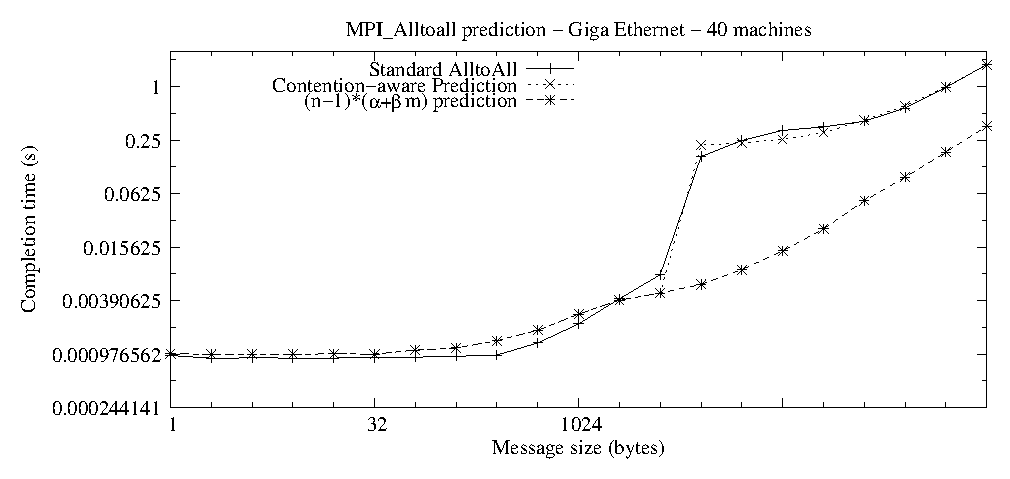
\includegraphics[width=0.7\columnwidth]{images/newcomp24_pred_log}
	\caption{\label{Figure: local}Performance mesurée et modélisée pour le MPI\_Alltoall dans un réseau Gigabit Ethernet}
\end{figure}


Vu la précision de ce modèle pour les \textit{clusters} homogènes, notre première réaction serait de l'appliquer aussi dans le cas des \textit{grids} de calcul en faisant la somme des performances des réseaux locaux et distants (Équation \ref{eq:7}). Malheureusement cette stratégie n'aboutit pas car les performances observées sont largement inférieures à celles prévues par ce modèle, comme indique la Figure \ref{Figure: standard}. 

\begin{equation}
T=max(T_{\mathcal C_1},T_{\mathcal C_2})+max(n_1, n_2) \times (\alpha_w+\beta_w \times m)
\label{eq:7}\end{equation}

En effet, la figure \ref{Figure: standard} représente des mesures effectuées entre deux \textit{clusters}, l'un situé à Nancy et l'autre à Rennes. Les deux \textit{clusters} étaient constitués de machines similaires (dual Opteron 246, 2 GHz) interconnectées localement par un réseau Gigabit Ethernet, alors que le lien \textit{inter-cluster} était un réseau privé de 10 Gbps. Les mesures ont été obtenues selon la méthode \emph{broadcast-barrier} \cite{Supinski99}.


\begin{figure}
	\centering
	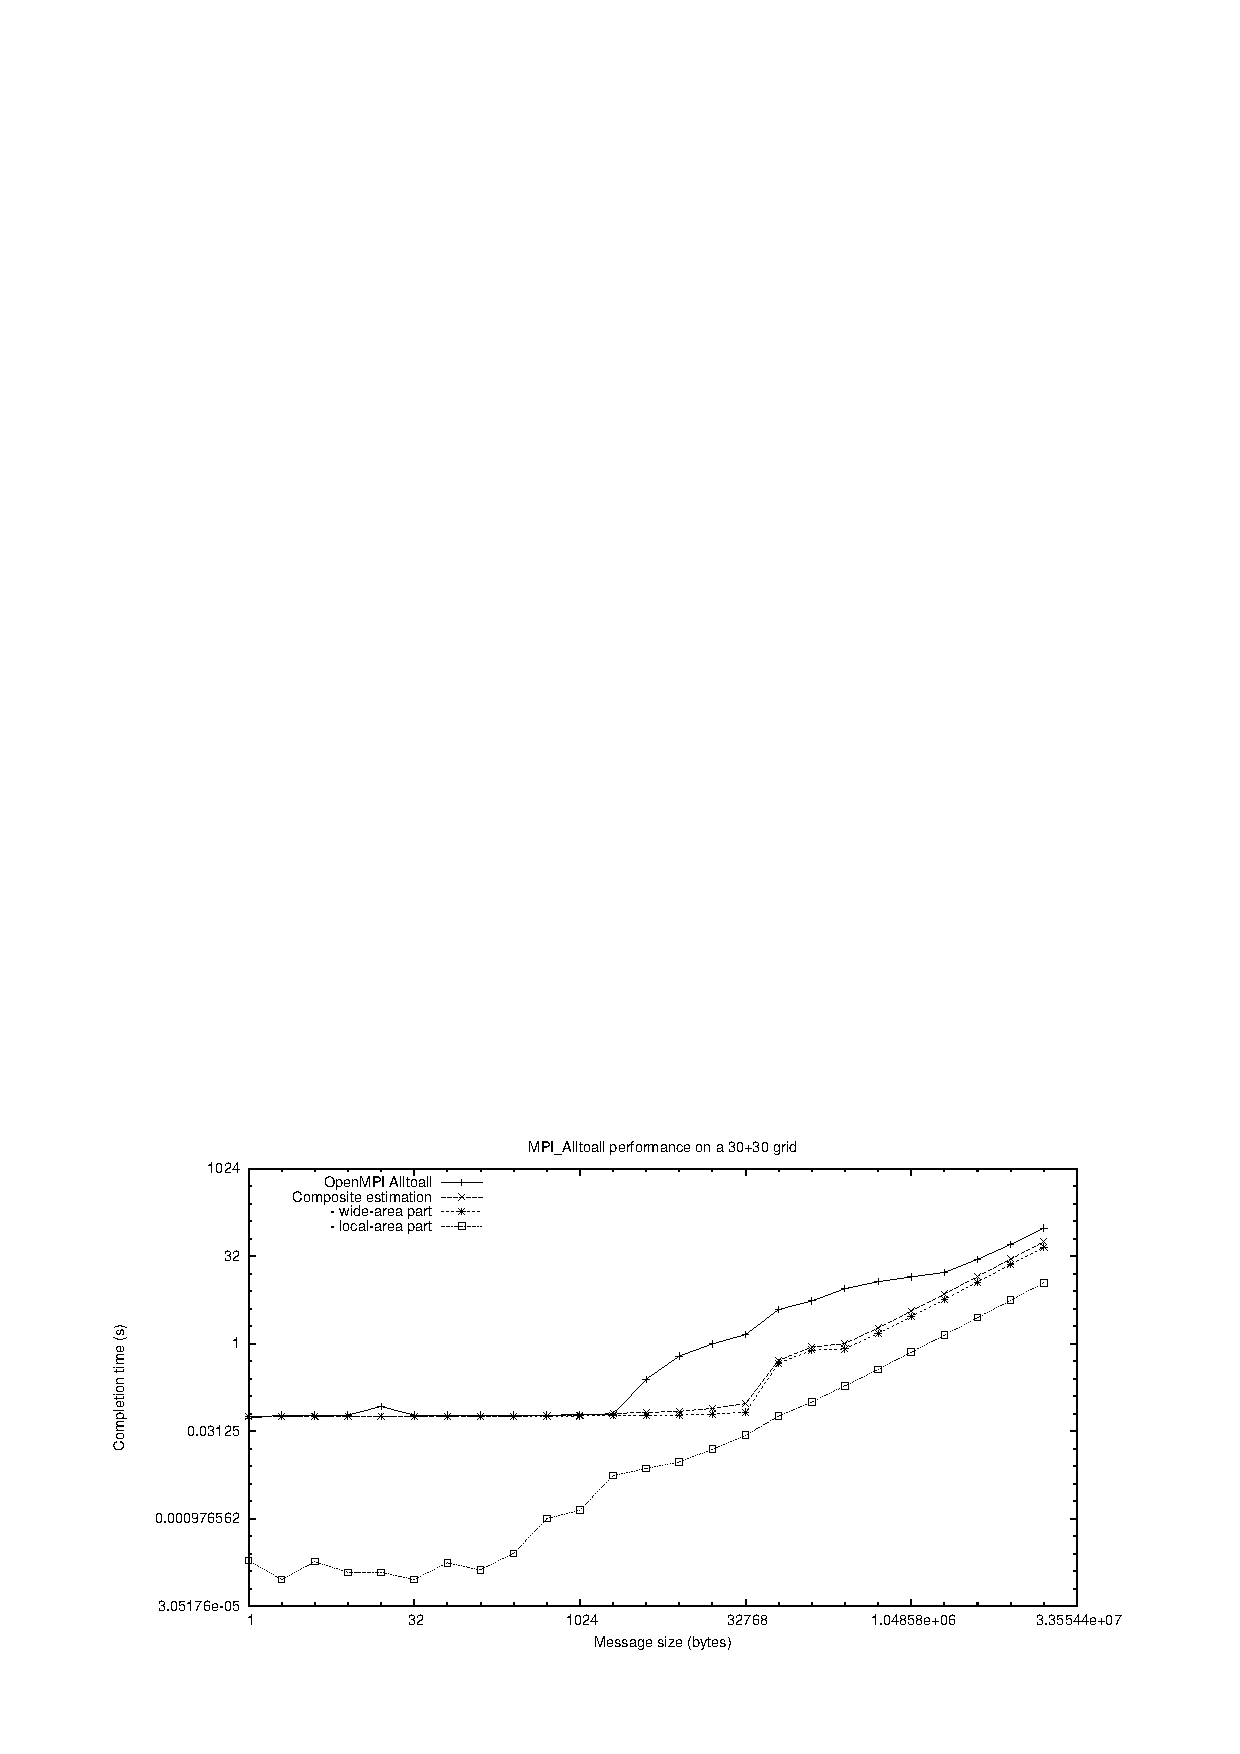
\includegraphics[width=0.7\columnwidth]{images/standard}
	%\vspace{-0.5cm}
	\caption{\label{Figure: standard}Performance mesurée et modélisée pour le MPI\_Alltoall dans un \textit{grid}} %\vspace{-0.5cm}
\end{figure}
 
Bien qu'on pourrait rajouter des paramètres supplémentaires pour s'approcher des performances observées, nous avons décidé d'attaquer le problème directement à sa source en optimisant la façon dont les communications sont effectuées sur un \textit{grid}. 


\subsection{All-to-All pour les \textit{Grids} : l'algorithme LG}

Lors de l'opération dans un \textit{grid}, l'un des facteurs les plus importants à prendre en compte est le temps nécessaire à ce que les messages soient livrés car ceux-ci sont affectés par la distance géographique mais aussi par l'hétérogénéité des protocoles, le routage des messages et les interférences des autres flux rencontrés sur le backbone. 

La plupart des algorithmes pour les communications collectives sur les \textit{grids} (PACX MPI~\cite{Gabriel98}, MagPIe~\cite{Kielmann01}) visent la minimisation des communications à grande distance en choisissant un coordinateur dans chaque \textit{cluster} qui sera responsable par les échanges \textit{intra-cluster}. Bien que ce mécanisme présente des avantages pour d'autres patrons de communication, il n'est pas adapté aux opérations de type  MPI\_Alltoall. En premier lieu, ce mécanisme  induit des étapes de communication supplémentaires du fait de forcer le passage par les coordinateurs des \textit{clusters}, qui de plus deviennent des goulots d'étranglement. En deuxième lieu, cette approche n'est pas optimale par rapport à l'utilisation des liens \textit{inter-cluster}, souvent capables de supporter des flux multiples \cite{Casanova05}. 

Afin de mieux traiter ce problème, nous essayons de minimiser les échanges distants d'une autre manière. En effet, la grande complexité des échanges du All-to-All réside dans les différentes performances des liens locaux et distants, or les implémentations traditionnelles de MPI\_Alltoall sont incapables de faire la différence. Si nous pouvons identifier la disposition des n{\oe}uds, on peut utiliser toutes les machines d'un \textit{cluster} pour collecter les données à un niveau local avant de les envoyer simultanément au réseau distant, en une unique étape de communication. 

Ainsi, le mécanisme que nous avons proposé en \cite{Steffenel07c} est une solution "\textit{grid aware}" qui s'exécute en deux étapes. Dans un premier moment, seulement les échanges locaux sont effectués. Cette phase inclut les échanges attendus entre les n{\oe}uds \textit{intra-cluster} mais aussi l'échange des données destinés aux autres \textit{clusters}, stockés dans des buffers supplémentaires pour la deuxième phase. L'avantage de cet échange est que son coût est très faible par rapport au coût d'une communication distante (voir Figure \ref{Figure: standard}). Finalement, lors de la deuxième phase, les buffers sont transmis directement aux n{\oe}uds destinataires, complétant ainsi l'échange total.  

Plus exactement, l'algorithme peut être décrit comme suit. Sans perte de généralité, considérons un \textit{cluster}  ${\mathcal C}_1$ qui contient moins de n{\oe}uds que le \textit{cluster} ${\mathcal C}_2$ ($n_1\leq n_2$). Les n{\oe}uds sont ainsi numérotés de 0 à $n_1+n_2-1$, avec les n{\oe}uds allant de 0 à $n_1-1$ appartenant à ${\mathcal C}_1$ et les n{\oe}uds allant de $n_1$ à $n_1+n_2-1$ appartenant au \textit{cluster} ${\mathcal C}_2$. Nous appelons ainsi ${\mathcal M}_{i,j}$ le message (donnée) qui sera envoyé du n{\oe}ud $i$ au n{\oe}ud $j$. 

L'algorithme suit les deux étapes : 
\begin{description}
	\item[Première étape] Pendant cette phase, nous effectuons les échanges locaux : Le n{\oe}ud $i$  envoie ${\mathcal M}_{i,j}$ au n{\oe}ud $j$, seulement si $i$ et $j$ font partie du même \textit{cluster}. Ensuite, ils préparent les buffers pour les communications distantes de manière à ce que les données à destination d'un n{\oe}ud distant $j$ on ${\mathcal C}_2$ seront d'abord stockés sur le n{\oe}ud $j~ mod~ n_1$ de ${\mathcal C}_1$. De même, les données sur un n{\oe}ud $i$ de ${\mathcal C}_2$ à destination de $j$ sur ${\mathcal C}_1$ seront stockés sur le n{\oe}ud $ \lfloor i/n_1 \rfloor \times n_1 + j $.
	\item[Deuxième étape] Pendant cette deuxième étape, seulement $n_2$ communications \textit{inter-cluster} auront lieu. Cette phase est décomposée en $\lceil n_2/n_1\rceil$ vagues avec $n_1$ communications chacune. Ainsi, pendant la vague $s$, le n{\oe}ud  $i$ de ${\mathcal C}_1$ échangera son buffer local avec le n{\oe}ud $j=i+n_1\times s$ de ${\mathcal C}_2$ (si $j < n_1+n_2$). Plus exactement, $i$ envoie  ${\mathcal M}_{k,j}$ à $j$ où $k\in [0,n_1]$ et $j$ envoie ${\mathcal M}_{k,i}$ à $i$ où $k\in[n_1\times s,n_1\times s+n_1-1]$.
\end{description}

Comme cet algorithme minimise le nombre de communications \textit{inter-cluster} et les organise par vagues, nous n'avons besoin que de $2\times \max(n_1,n_2)$ messages dans les deux directions (par rapport à  $2\times n_1 \times n_2$ messages dans l'algorithme traditionnel). Si les deux \textit{clusters} ont le même nombre de n{\oe}uds, une seule vague d'échanges sera nécessaire. Notre algorithme est aussi optimisé sur la longue distance car il regroupe plusieurs messages ensemble, réduisant l'impact de la latence et des interférences sur le backbone. La Figure \ref{Figure: comp} présente une comparaison entre la performance de l'algorithme traditionnel implémenté par OpenMPI et celle de l'implémentation de l'algorithme ${\mathcal LG}$. Nous observons que l'algorithme ${\mathcal LG}$ obtient un gain de performance de presque 50\% par rapport à la stratégie traditionnelle.

\begin{figure}
	\centering
	\includegraphics[width=0.7\columnwidth]{images/comp}
	\caption{\label{Figure: comp}Comparaison de performance entre OpenMPI et l'algorithme ${\mathcal LG}$}
\end{figure}

L'ordonnancement des communications effectué par ${\mathcal LG}$ a aussi une conséquence sur la modélisation des performances. Tout d'abord, il minimise les communications de longue distance, réduisant les risques de congestion qui sont difficiles de modéliser. De plus, la transmission groupée des messages réduit l'impact de la latence et des fluctuations de performance du réseau. C'est ainsi que nous avons pu établir un modèle composé des performances locales (${\mathcal T_{C_{n}}}$, obtenues à partir de l'équation \ref{eq:6}) et des prédictions pour les communications de longue distance obtenues par les méthodes traditionnelles :

\begin{equation}
T=max(T_{\mathcal C_1},T_{\mathcal C_2})+\lceil n_2/n_1\rceil \times (\alpha_w+\beta_w \times m \times n_1)
\label{eq:8}\end{equation}

Afin d'obtenir les paramètres nécessaires aux prédictions, nous avons utilisé la procédure décrite par Kielman \textit{et al.} \cite{Kielmann00}. Les facteurs de contention $\gamma=2.6887$ et $\delta=0.005039$ pour $M>=1KB$ ont été obtenus par la méthode des moindres carrés comme décrit par \cite{Steffenel06b}.

\begin{figure}
	\centering
		\includegraphics[width=0.7\columnwidth]{images/simul}
	\caption{\label{Figure: simul}Performance de ${\mathcal LG}$ et sa prédiction}
\end{figure}

La Figure \ref{Figure: simul} compare ainsi les prédictions obtenues avec l'Équation \ref{eq:8} et les performances mesurées pour l'algorithme ${\mathcal LG}$. Nous observons une bonne adéquation des prédictions, ce qui était impossible avec l'implémentation traditionnelle de MPI\_Alltoall. 

\section{Bilan et Perspectives}

Les travaux présentés dans ce chapitre prouvent l'intérêt de la modélisation des communications dans les réseaux hétérogènes, autant pour la prédiction des temps de communication que pour l'optimisation des algorithmes existants. Ceci est démontré notamment dans le cas de l'algorithme $LG$, qui a vu le jour uniquement parce que l'observation et la modélisation des performances indiquait des situations non-optimales dans les échanges entre deux \textit{clusters}.

Au fil des années mes intérêts se sont diversifiés et la modélisation des performances telles que présentées dans ce chapitre ne sont plus si fréquentes. Dans la plupart des cas mes travaux visent la comparaison des performances entre différentes approches logiciel et environnements d'exécution, ou bien l'amélioration des performances des applications grâce à la parallélisation de certaines routines. Ceci est le cas de deux travaux effectués récemment:

\subsubsection*{Utilisation de GPUs pour Augmenter la Performance d'une Application de \textit{Data Mining}}

Dans ces travaux effectués en collaboration avec Andrea Charão et Tiago Engel (Universidade Federal de Santa Maria, Brésil), nous nous sommes intéressés à l'optimisation des performances d'une application de \textit{data mining} et \textit{machine learning }très connue, Weka\footnote{\url{https://www.cs.waikato.ac.nz/ml/weka/}}. 

Bien que les termes \textit{data mining} et \textit{machine learning} soient fréquemment associés au \textit{big data}, on retrouve encore un nombre assez important d'applications et outils qui ne sont pas parallélisés ni s'exécutent sur un \textit{cluster} ou une infrastructure hébergée sur \textit{cloud}. Le plus souvent ceci est dû au fait que les masses de données ne sont pas tellement importantes pour avoir recours à des infrastructures plus puissantes, ou tout simplement car des instances moins importantes des données sont utilisées pour explorer et étudier un problème avant son déploiement.

Weka est un environnement très connu des chercheurs en \textit{data mining}, souvent utilisé pour l'apprentissage des techniques de classification, régression, clusterisation, etc. Weka est aussi une bibliothèque qui peut être intégrée aux application.  

Dans le cadre de ce travail nous avons constaté que la plupart des opérations sur Weka ne sont pas parallélisés (ni sur les multiples c{oe}urs de la CPU, ni sur un accélérateur GPU). En choissant les bonnes routines, nous croyons pouvoir améliorer sensiblement la performance de cette plateforme.

Grâce à l'étude des profiles d'exécutions lors de l'exécution d'une application métier (étude d'images de mammographie afin d'identifier des possibles sites tumoraux), nous avons pu déterminer un petit nombre d'opérations qui consommaient la plupart du temps de calcul. Ainsi, nous avons étudié le remplacement de ces opérations par des versions multi-c{oe}ur et GPU, avec comme résultat une réduction de plus de 50\% du temps d'exécution de l'application \cite{Engel14a,Engel2015}.

En ce moment nous poursuivons ces collaborations avec l'étude des performances d'accès aux services cloud \cite{Charao17a}  ou en associant des étudiants, comme par exemple les deux articles publiés récemment au Brésil (\cite{Nesi17a, Muenchen17a}) et conduits dans le cadre du projet de collaboration international CAPES-Cofecub MESO.

\subsubsection*{Évaluation des Performances de la Virtualisation sur les Dispositifs SoC (\textit{System on a Chip})}

Ce travail est le résultat d'une collaboration plus récente avec David Beserra, doctorant à l'Université Paris 1. L'objectif ici est d'étudier les dispositifs SoC comme par exemple les Raspberry Pi, Banana Pi, etc. par rapport à leur capacité d'exécuter des machines virtuelles de type conteneur (par exemple LXC ou Docker). En effet, une application fréquemment citée pour ces dispositifs est celui de n{oe}ud de proximité dans un réseau \textit{fog computing}, et une meilleure compréhension du support à la virtualisation dans ces dispositifs peut aider le déploiement et la migration d'applications et de micro-services.

Des campagnes de mesure et d'analyse des performances ont été conduits lors de la première année de thèse de M Beserra, et ont donné lieu à deux publications dans des conférences internationales \cite{Beserra17a, Beserra17b}. La suite des travaux vise l'étude des plates-formes de micro-services, on espère bientôt pouvoir effectuer des nouvelles campagnes d'expérimentation.

\chapter{L'Hétérogénéité des Tâches de Calcul}

% !TeX spellcheck = fr_FR
\begin{resume}
La gestion de l'hétérogénéité peut (et doit) être considérée sous plusieurs aspects. Alors que le chapitre précédent a donné des exemples de travaux dans lesquels l'étude sur l'hétérogénéité s'était concentrée sur les aspects liés à la communication, dans ce chapitre nous nous concentrons sur l'hétérogénéité du calcul. Ce type d'hétérogénéité est souvent le plus simple à traiter car le plus fréquent : il est presque impossible développer une application parallèle où les tâches de calcul sont parfaitement régulières. Bien, sûr, la gestion des tâches régulières ou irrégulières dépend de leur interdépendance. Plus elles sont découplées, moins on trouve de contraintes pour leur exécution, ce que simplifie leur gestion.

Dans ce chapitre nous considérons que les tâches de calcul sont hétérogènes si les différentes tâches d'une application présentent des variabilités dans leurs temps d'exécution à cause des facteurs propres à chaque tâche : variations dans le volume ou nature des données à traiter, variations de la complexité des opérations à effectuer, etc. Contrairement au chapitre précédent, nous n'essayons pas de modéliser les performances ou les prédire, mais simplement essayons d'appliquer des mécanismes de gestion des tâches dans le cas de la parallélisation d'une application métier et de son déploiement sur un cluster de calcul.

Ainsi, ce chapitre démarre avec la description d'une application destinée à l'exécution de problèmes d'amarrage moléculaire. Nous devons la rendre parallèle pour mieux la déployer à plus grande échelle, sans toutefois modifier son code source. Les prochaines sections détaillent donc les spécificités de l'application métier et les approches retenues pour découper les instances de calcul en unités pouvant être traitées en parallèle. Ensuite, on présente deux stratégies de gestion des tâches qui ont été implémentées, destinées nos seulement à garantir le bon déroulement du calcul et le regroupement des résultats mais aussi destinées à mieux utiliser les ressources disponibles dans les environnements de calcul.

Le travail décrit dans ce chapitre a été développé dans le cadre de la codirection de thèse de Romain Vasseur (thèse en bio-informatique, dirigée par le prof. Manuel Dauchez et co-encadré par Stéphanie Baud et moi-même). Cette thèse, effectuée entre 2012 et 2015, était une thèse CIFRE portée par le Laboratoire MeDyC - Matrice Extracellulaire et Dynamique Cellulaire (UMR CNRS 7369), le laboratoire CReSTIC (EA - 3804) et la compagnie Bull-Atos. Ces travaux ont fait l'objet de publication de 2 articles en journaux internationaux, 2 conférences internationales (dont un "\textit{Best Paper Award}") et 3 communications courtes (posters et résumés).

\end{resume}

\section{Hétérogénéité du Calcul - application à la recherche en amarrage moléculaire} \label{sec:Vasseur}

L'utilisation d'approches informatiques pour identifier les interactions biomoléculaires est devenu l'un des principaux piliers de la recherche de nouvelles drogues et principes actifs. En effet, la simulation \emph{in silico} permet de faire une première prospection sur un grand nombre de candidats potentiels, tout avec un gain de temps important et un coût nettement moins onéreux que l'expérimentation \emph{in vitro}. 

L'amarrage moléculaire (aussi appelé \emph{docking moléculaire}) est donc une technique qui vise à étudier les interactions au niveau moléculaire entre certaines structures du vivant, comme par exemple les interactions protéine-ADN/ARN, protéine-protéine, peptides-protéine, protéine-ligand ou glucide-protéine. L'industrie pharmaceutique s'intéresse particulièrement à l'étude des interactions protéine-ligand, notamment la recherche de principes actifs de médicaments (ligands) qui puissent se connecter à certaines protéines cible. La prédiction des modes d'amarrage d'un ligand à une protéine, la structure du complexe résultant et l'estimation de l'affinité de cet amarrage sont essentiels pour le développement de nouveaux composés thérapeutiques, et les méthodes numériques ont été le choix principal de plusieurs travaux dans la littérature \cite{Abagyan2001,Giganti2010, Klebe2006}.

 Souvent cette étude se fait à travers un "criblage virtuel" (\emph{virtual screening}), qui consiste en un déploiement à grande échelle permettant de tester un grand nombre de ligands (de centaines à plusieurs millions selon l'ampleur de la campagne) sur un nombre très restreint de cibles. En effet, nous trouvons des millions de composants catalogués dans des bases de données telles que la Cambridge Structural Database \cite{Allen2002}, PDBbind  \cite{Wang2004, Wang2005}, ZINC \cite{Irwin2005} et tant d'autres collections privées des groupes pharmaceutiques. De même, un riche catalogue de protéines peut être obtenu à partir du Research Collaboratory for Structural Biology (RCSB) Protein Data Bank (PDB) \cite{PDB}, une base de données ouverte qui contient plus de 120 000 protéines cataloguées et qui est enrichie de plus de 7000 nouvelles protéines par an. Ainsi, un chercheur ou un industriel qui souhaite activer ou désactiver une protéine afin de combattre une maladie peut donc effectuer ce criblage virtuel entre la protéine cible et les milliers de ligands catalogués (enzymes, peptides, etc.).  

Dans le cadre des travaux de thèse de Romain Vasseur nous nous sommes penchés sur le développement et l'exécution parallèle d'une application pour le criblage moléculaire inversé. Plus exactement, un criblage inversé a pour objectif de discriminer les cibles protéiques les plus favorables à une interaction avec le ligand, parmi un échantillon de structures de protéines plus ou moins important. De cette manière, il est possible d'identifier des cibles secondaires pour un ligand développé, ou bien faire une étude préalable des risques d'interactions indésirables. 

\subsection{Travaux Proches et Méthodologie de Parallélisation}

Le terme \textit{inverse docking} a fait son apparition dans la littérature en 2001 avec les deux articles de Chen \textit{et al}. \cite{Chen2001,Chen2001b}. Une quinzaine d'articles ont été recensés depuis cette date, avec des méthodes de traitement à plus ou moins grande échelle. La plupart de ces travaux font l'usage d'applications pour le docking traditionnel telles que AutoDock \cite{Steffen07} ou AutoDock Vina \cite{Lauro2011,Lauro2012}, avec très peu d'outils dédiés exclusivement au docking inversé (INVDOCK \cite{Chen2001,Chen2001b} ou TarFisDock \cite{Li2006}). Toutefois, aucun de ces articles ne décrit ni ne mentionne le développement d'une méthode de déploiement sur des architectures de type HPC.

Ainsi, nous avons développé nos propres stratégies dans le but de pouvoir traiter des centaines en parallèle de protéines grâce aux architectures HPC.
Ces stratégies concernent la parallélisation du calcul d'un couple ligand-protéine mais aussi le déploiement large échelle de ces calculs. 

Dans ce travail nous sommes parti de la méthode appelée \textit{blind docking} qui consiste à détecter des points d'amarrage possibles en faisant un balayage sur l'ensemble de la surface de la protéine. Pour cela, des applications telles que Autodock doivent générer une grille d'affinités basée sur les énergies de liaison de chaque atome qui compose la protéine. Cette grille d'affinité se présente comme une boîte 3D qui contient toute la surface de la protéine, plus une marge afin de permettre le placement d'un ligand à l'intérieur de la boîte. Par la suite, un algorithme génétique ira explorer le volume autour de la protéine afin d'évaluer l'énergie de liaison à différents endroits. 

L'approche \textit{blind docking} est naïve et difficilement parallélisable car chaque pair protéine-ligand représente une boîte et donc une tâche de calcul Autodock. De plus, selon les caractéristiques de la protéine, un nombre important d'itérations (générations dans l'algorithme génétique) sont nécessaires pour couvrir systématiquement la surface de la protéine et permettre l'obtention de résultats satisfaisants. Comme résultat, l'exécution d'une seule instance du \textit{blind docking} avec l'application AutoDock peut prendre plusieurs heures. Malgré ces contraintes, cette approche est assez répandue et a donc été utilisée comme référence de comparaison pour les approches parallèles que nous avons développées.

\section{Parallélisme Intérieur : décomposition des tâches}
Afin d'optimiser l'utilisation des ressources de calcul lors d'une campagne de docking inversé, il est impératif d'intégrer le parallélisme au c{\oe}ur du traitement des tâches de calcul, comme illustré en figure \ref{fig:romain-fig1}. La décomposition d'une instance de docking permet une meilleure utilisation des ressources de calcul en distribuant les tâches sur plusieurs machines, mais aussi grâce à un traitement en pipeline qui permet l'enchaînement des opérations lorsque certaines tâches finissent plus tôt. De plus, cela rend l'exécution plus tolérante aux fautes, une tâche qui a été interrompue peut être redéployée sur une autre machine sans obliger le redémarrage de toute l'exécution. Dans le cadre de ce travail, nous avons étudié les techniques de décomposition présentées dans les sections suivantes. 

\begin{figure}
	\centering
		\includegraphics[width=0.65\linewidth]{images/Romain/fig1-color}
	\caption{Exemple d'un schéma de décomposition parallèle}\label{fig:romain-fig1}
\end{figure}

\subsection{Décomposition Géométrique Arbitraire}
Vu la nature des données utilisées en entrée pour le docking, nous avons initialement étudié une stratégie de décomposition géométrique qui consiste à découper la grille d'affinité 3D en plusieurs boîtes plus petites, chacune couvrant un secteur de la protéine. Cette stratégie considère une décomposition géographique régulière de telle manière que le nombre de tâches (boîtes) ont une taille similaire, permettant ainsi la génération de $n^3$ sous-grilles : 8 (2x2x2), 27 (3x3x3), 64 (4x4x4), etc. Le choix du bon nombre de découpages dépend à la fois du gain  en parallélisme mais aussi de la liberté de mouvement du ligand à l'intérieur d'une grille. 
En effet, on peut espérer un gain de performance du fait de pouvoir déployer en parallèle les différentes sous-grilles comme des tâches de calcul indépendantes. Toutefois, un nombre trop important de découpages aura pour effet la génération de sous-grilles "inutiles" car elles couvrent que des zones inaptes à la recherche de points d'amarrage (espace non connecté à la surface de la protéine, "intérieur" de la protéine, etc.). De plus, une boîte 3D trop petite peut empêcher le positionnement du ligand et donc rendre l'évaluation de l'amarrage impossible.

Un autre inconvénient de cette technique est que le découpage se fait de manière arbitraire, sans prendre en compte les spécificités de la surface de la protéine. Par exemple, les "cavités" présentes dans la surface de la protéine sont souvent des bons sites pour l'amarrage, mais un découpage arbitraire qui l'ignore peut simplement scinder cette cavité en deux et la rendre bien moins intéressante vis-à-vis de l'algorithme de docking. De même, l'évaluation de docking se fait en considérant que le ligand se trouve totalement à l'intérieur de la sous-grille : n'importe quelle conformation où des atomes ligand dépassent la grille serait invalide et donc ignorée. 

\subsection{Décomposition Géométrique avec Superposition}
Les inconvénients de la décomposition géométrique arbitraire cités dans la section précédente nous ont conduit à développer une technique alternative de découpage qui préserve la liberté de placement des ligands et permet une couverture intégrale de la surface de la protéine. Cette technique consiste à effectuer un découpage avec superposition entre les sous-grilles voisines, de manière à pouvoir évaluer le placement du ligand même sur les zones proches des bords des sous-grilles. Bien sûr, cette superposition est dépendante de la taille des ligands, permettant ainsi une configuration qui optimise l'utilisation des ressources pour chaque pair protéine-ligand. 

Ainsi, dans le cadre du travail effectué, nous avons considéré deux valeurs de référence pour la superposition. La superposition entre deux boîtes serait d'un tiers de la longueur de la boîte si la longueur du ligand est inférieure à cela. Dans le cas contraire, la superposition correspond à la longueur du ligand. Grâce à cette configuration, le ligand a une liberté complète de placement (rotation, translation, etc.) et on peut effectuer une recherche exhaustive sur l'espace d'amarrage. Dans l'exemple illustré dans les prochaines sections nous utilisons aussi un schéma de décomposition en douze parties, 3x2x2 (où 3 correspond à l'axe principal de la protéine) et avec une superposition d'1/3 sur chaque sous-grille. 

\subsection{Recherche de Cavités}
Comme indiqué précédemment, l'amarrage des ligands est favorisé par la présence de cavités dans la surface de la protéine \cite{Ghersi2009,Hetenyi2011}, or les méthodes de découpage par décomposition ne prennent pas ces facteurs en compte. En effet, même avec la décomposition avec superposition, l'algorithme génétique utilisé pour la recherche de points d'amarrage ne fait que parcourir la surface sans un objectif précis. 

Nous pouvons améliorer la précision de notre docking inversé en effectuant la détection des zones avec cavités, par exemple à l'aide d'un programme dédié à ce fin, l'application Fpocket \cite{Guilloux09a}. La prise en compte des zones avec un plus grand potentiel peut augmenter la performance du docking inversé car cela nous permet de concentrer la recherche sur une zone plus spécifique. L'inconvénient est que son application nécessite un réglage fin des paramètres afin d'inclure les spécificités des protéines et de ne pas exclure des zones avec un potentiel moindre mais réel. 

Ainsi, au lieu de se reposer uniquement sur la recherche de cavités, notre travail a misé sur la complémentarité entre celle-ci et la décomposition géométrique avec superposition. En plus de générer des tâches de calcul pour les différentes sous-grilles issues de la décomposition géométrique, nous générons aussi des recherches ciblées sur les cavités identifiées par FPocket. Ces paramètres permettent une meilleure couverture des zones avec un plus grand potentiel (car couvertes par les deux techniques), tout en limitant le nombre de tâches de calcul supplémentaires.


\section{Gestion et Déploiement des Tâches de Calcul}

Les techniques de découpage présentées dans la section précédente permettent la parallélisation du traitement d'un couple protéine-ligand. Dans le cas du docking inversé, ce parallélisme dit "interne" doit être associé à la génération et au traitement des multiples tâches de calcul issues de chaque combinaison entre un ligand cible et la base de données de protéines recherchée. Enfin, les tâches de préparation des données (génération des sous-grilles, définition des paramètres, regroupement des résultats, etc.) doivent aussi être prises en compte. 

Il faut noter que la présence de tâches de différentes natures (préparation des grilles, criblage virtuel, détection de cavités) rendent la gestion des tâches un peu moins évident. Même les tâches de nature similaire peuvent présenter des variations selon la nature des données à traiter. Si nous prenons par exemple les tâches de criblage virtuel, le temps d'exécution dépend du degré de liberté des peptides à l'intérieur des boîtes 3D : une boîte découpée "à l'intérieur" de la protéine n'aura aucune surface exploitable et sera rapidement écartée.    

Pour toutes ces raisons, nous avons créé deux implémentations visant la gestion et le déploiement des tâches, toutes les deux intégrées à l'outil AMIDE \cite{Vasseur2015}. Dans le premier cas, une plate-forme générique qui gère tout seule l'ensemble des tâches a été conçue. Dans le deuxième cas, une partie des responsabilités est déléguée aux gestionnaires de tâches des clusters, simplifiant ainsi son exécution dans les environnements déjà pourvus de tels outils.

\subsection{Plate-forme Générique}

Vu les besoins de parallélisme interne et externe, nous avons dans un premier moment spécifié et développé une plate-forme générique basée sur le langage Python et capable d'exploiter le parallélisme multi-c{\oe}ur et multi-machine pour le docking inversé. 

Ainsi, un ensemble de scripts Python a été créé afin d'automatiser toutes les étapes liées à la préparation et à l'exécution du docking inversé. Parmi ces étapes nous pouvons citer :
\begin{itemize}
	\item[\textbf{(i)}] l'acquisition des fichiers PDB qui décrivent les protéines et ligands, 
	\item[\textbf{(ii)}] la préparation des fichiers PDB afin de sélectionner les structures cible, 
	\item[\textbf{(iii)}] l'extraction des coordonnées pour la création des grilles d'affinité, 
	\item[\textbf{(iv)}] la décomposition des grilles et 
	\item[\textbf{(v)}] le déploiement des tâches de calcul. 
\end{itemize}

Les étapes (i) et (ii) concernent majoritairement la manipulation de fichiers et le \textit{parsing} des informations, alors que les étapes  (iii) et (iv) sont liées à l'exécution de Autogrid, un outil qui fait partie de la suite Autodock et qui permet la création des grilles pour le docking. Selon la stratégie de décomposition retenue, l'étape (iv) peut créer une ou plusieurs grilles correspondant au découpage 3D. Dans le cas où l'on rajoute l'approche par recherche de cavités, il faut rajouter des grilles 3D générées  autour des zones identifiées par le logiciel Fpocket. 


\begin{figure}
	\centering
		\includegraphics[width=0.5\linewidth]{images/Romain/fig3-color}
	\caption{Représentation du flot d'exécution dans l'architecture distribuée}\label{fig:romain-fig3}
\end{figure}


Pour cela, la plate-forme utilise une architecture distribuée maître-esclave avec gestion d'une file d'exécution contenant les identifiants des tâches (task ID) et accessible en mode "sac de tâches" (\textit{bag of tasks} en anglais). Grâce à cette stratégie, les différents esclaves obtiennent une ou plusieurs tâches à exécuter, selon le nombre de c{\oe}urs de calcul disponibles. Pour être plus exacte, dans cette architecture nous trouvons deux files d'exécution, l'une dédiée à la préparation des sous-grilles et l'autre dédiée à l'exécution des tâches de docking. La première file est alimentée par le maître qui, à partir des paramètres d'entrée, indique aux esclaves les différentes protéines à analyser et aussi les stratégies de découpage à mettre en place, ainsi que la génération des sous-grilles avec l'outil Autogrill de la suite Autodock. Les esclaves doivent d'abord finir toutes les tâches dans cette file avant de passer à la file suivante.

Pour plus d'efficacité, la deuxième file d'exécution n'est plus alimentée par le maître mais directement par les esclaves. Lorsque ceux-ci finissent la préparation d'une tâche de la première file, il suffit de déposer le TaskID correspondant dans la deuxième file d'exécution. La Figure \ref{fig:romain-fig3} illustre le flot d'exécution de ces deux étapes.  


\subsection{Optimisation aux Clusters HPC}

 L'architecture distribuée présentée ci-dessous est adaptée à une exécution sur tout type de réseau d'ordinateurs (cluster, cloud, grid pervasif, etc.). Toutefois, il est possible d'optimiser son fonctionnement sur les clusters HPC si on prend en compte l'existence d'un gestionnaire de tâches propre à ces systèmes. En effet, la plupart des clusters HPC fait l'usage d'un gestionnaire de tâches afin de garantir la réservation et l'équité d'usage des ressources. Des systèmes tels que PBS \cite{Henderson95}, OAR \cite{Capit2005} ou Slurm \cite{Yoo2003} sont capables de gérer plusieurs files d'exécution ainsi que de déployer des tâches en mode \textit{best effort} de manière à occuper les ressources de calcul lorsque les réservations ne suffisent pas. 
 
 Dans le cas de l'optimisation pour les clusters HPC notre stratégie a été d'éliminer la dépendance vis-à-vis d'un n{\oe}ud maître et permettre ainsi l'exécution des tâches indépendantes selon les disponibilités du gestionnaire de tâches. En effet, la présence d'un n{\oe}ud maître était nécessaire afin de gérer les files d'exécution mais aussi de vérifier la terminaison des tâches (garantissant la tolérance aux fautes). Cela oblige donc que le processus maître reste actif pendant toute l'exécution, ce qui impose des problèmes lors de la réservation des ressources destinées au maître (combien de temps faut-il le garder actif ?). Cette limitation est encore plus importante dans le cas d'un déploiement \textit{best-effort}, où la terminaison des tâches risque d'être fortement étalée au gré de l'occupation des ressources. Comme les gestionnaires de tâches des clusters HPC sont capables de détecter une tâche interrompue et la relancer, il suffit de soumettre dans une même tâche les paramètres nécessaires à la génération des sous-grilles et à leur docking. 
 
 Grâce à cette optimisation, l'outil AMIDE issu de ces travaux est capable d'effectuer le docking inversé autant dans un cluster que dans un agglomérat de machines indépendantes.
 
 \section{Évaluation Pratique}
 
 Lors de la mise en place de l'outil AMIDE nous avons exécuté plusieurs expériences dans le but de valider notre approche de travail. L'un de ces tests consistait à évaluer la précision des stratégies de décomposition en étudiant un complexe ligand(X23)-protéine(3CM2) bien connu dans la littérature. La comparaison s'est fait par rapport à la technique classique du \textit{blind docking} mais aussi par rapport à des données expérimentales obtenues par cristallographie. Dans un deuxième moment, nous avons conduit des tests de performance dans lesquels le docking inverse était déployé sur un large ensemble de protéines issues de la bibliothèque PDB.
 
Toutes les expériences ont été conduites sur le cluster Clovis du centre de calcul ROMEO à Reims. Clovis était un cluster hybride avec 36 n{\oe}uds Westmere-EP (12 c{\oe}urs), 2 n{\oe}uds Nehalem-EX (32 c{\oe}urs), un n{\oe}ud Westmere-EP (12 c{\oe}urs + 2 Fermi C2050 GPUs) et un n{\oe}ud Nehalem-EP (8 c{\oe}urs + GPU Fermi M2090), et au moins 2GB de mémoire par c{\oe}ur. Pour une question de régularité, les expériences ici présentées ont été lancées exclusivement sur les n{\oe}uds Westmere-EP. De plus, afin de mieux évaluer la communication intra-cluster, seulement 4 c{\oe}urs de calcul ont été utilisés par n{\oe}ud.
 
 Ainsi, pour la première expérience, nous avons initialement exécuté un blind docking de la protéine 3CM2 et du ligand X23. Comme illustré en  Figure \ref{fig:blind}, le blind docking a permis la détection de la cavité et d'une conformation presque identique à celle obtenue par cristallographie (différence RMSD de 1.60 Angstroms seulement).
 
 \begin{figure}[h]
 	\centering
 		\includegraphics[width=0.85\linewidth]{images/Romain/fig4-color} 
 		\caption{Placement du ligand selon la méthode cristallographique (rouge) et par blind docking (vert)}\label{fig:blind} %\vspace{-0.3cm}
 \end{figure}
 
 \begin{table}
 	\begin{center}
 		\caption{Tableau comparatif des précisions du docking de 3CM2 selon les stratégies de décomposition et le nombre d'itérations. La distance RMSD est comparée à la pose cristallographique et les énergies de liaison à celles obtenues par la méthode blind docking.}\label{tab:rmsd}
 		\begin{tabular}{|c|c|c|c|}
 			\hline 
 			$\Delta G$ blind docking & Nombre d'itérations & énergie de liaison $\Delta G$ & RMSD  \\ 
 			($kcal.mol^{-1}$)  &  & ($kcal.mol^{-1}$) &  (\AA{}) \\
 			\hline 
 			\multirow{3}{*}{$\Delta G = -10.27$}  & 20 & $\Delta G_{12} = -10.09$ & 1.79 \\ \cline{2-4}
 			& 50 & $\Delta G_{pocket} = -10.11$ & 1.86 \\ \cline{2-4}
 			& 70 & $\Delta G_{pocket} = -10.39$ & 1.62 \\ \cline{2-4}
 			\hline 
 		\end{tabular} 
 	\end{center}
 	%\vspace{-0.3cm}
 \end{table}
 
Le découpage avec le meilleur score d'énergie de liaison est celui en $n = 12$, comme illustré en Figure \ref{fig:cuts}. Avec seulement 20 itérations, ce type de décomposition a permis l'obtention d'un placement similaire à celui de la méthode blind docking (voir Table \ref{tab:rmsd}). Les autres formats de découpage ont réussi à placer le ligand dans la cavité cible, mais leurs résultats en termes d'énergie de liaison et de distance RMSD ne sont pas suffisants. La méthode de recherche de cavités a aussi permis le placement du ligand avec une bonne précision, au bout de 50 itérations. 


 
 \begin{figure}[h]
 	\centering
 		\includegraphics[width=0.85\linewidth]{images/Romain/fig5-bw} 
 		\caption{Comparaison entre la pose blind docking (a) et celle d'un découpage à $n=12$ (b) et par recherche de cavités (c). }\label{fig:cuts} %\vspace{-0.3cm}
 \end{figure}

\begin{figure}
	\centering
		\includegraphics[width=0.5\linewidth]{images/Romain/fig7-color}
		\caption{Comparaison des temps d'exécution pour les tâches issues des différentes méthodes de découpage}\label{fig:performance} %\vspace{-0.3cm}

\end{figure}

%\begin{figure}[h]
%	\begin{center}
%		\includegraphics[width=0.5\linewidth]{images/Romain/fig8-color} 
%		\caption{Distribution de la charge lors du docking de 5 protéines (la durée de chaque exécution est indiquée dans les blocks)}\label{fig:balance}\vspace{-0.5cm}
%	\end{center}
%\end{figure} 

 
Dans un deuxième moment nous avons effectué le docking inversé du ligand X23 sur un ensemble de 100 protéines issues de la base PDB. Ici, l'utilisation du découpage a permis une  meilleure utilisation des ressources grâce à l'équilibrage de charge %(voir Figure \ref{fig:balance}) 
mais aussi meilleure prise en charge de la tolérance aux fautes. En effet, la Figure \ref{fig:performance} affiche la durée moyenne d'exécution d'une tâche selon les différentes méthodes considérées dans ce travail. Ainsi, une exécution de type blind docking nécessitait plus de 5h30, et toute interruption oblige la réexécution complète de la tâche. À l'opposé, l'interruption d'une tâche issue d'une décomposition en 12 parties ne demande qu'une demi-heure de ré-exécution, en cas de défaillance.  


 

\section{Bilan et Perspectives} \label{sec:disc}

%todo falar do trabalho com o Tiago, que também visait a paralelisation e optimisation d'une application métier









\chapter{L'Adaptation à la Dynamicité des Ressources}

\begin{resume}
La gestion de l'hétérogénéité des ressources peut être considérée sous plusieurs aspects. Les chapitres précédents ont donné des exemples de travaux dans lesquels l'hétérogénéité s'était concentrée sur les communications (Chapitre \ref{Chap:MPI}) ou sur le couple données-communication (Chapitre \ref{SEC:GRAPPES}). Dans ce chapitre nous nous concentrons sur un troisième socle, celui de l'hétérogénéité de calcul. Plus exactement, ce chapitre présente des travaux dont les contributions ont visé la prise en charge de l'hétérogénéité des ressources de calcul ou l'hétérogénéité des tâches de calcul, tous les deux résultant en une variabilité des temps d'éxécution de tâches qui a dû être traitée et optimisée. Il est aussi important de remarquer que la communication et le stockage peuvent varier mais, dans ces cas, ils sont traités par des outils et mécanismes sous-jacents qui n'ont pas été la cîble de nos travaux.

Ainsi, ce chapitre démarre avec la description d'une plate-forme de calcul destinée à l'exécution de problèmes d'amarrage moléculaire. Ce travail, développé dans le cadre de la co-direction de thèse de Romain Vasseur, est un exemple d'application métier où l'environnement développée sert à déployer de manière distribuée une application déjà existante et dont le code source ne pourrait pas être facilement parallélisée. L'approche retenue a été composée d'une gestion distribuée d'instances de calcul sur un cluster/grappe, associée à un découpage plus fin du problème afin de multiplier les tâches de calcul et ainsi mieux utiliser les ressources disponibles.

La deuxième partie de ce chapitre décrit les efforts effectués dans le cadre du projet de collaboration international STIC-AmSud PER-MARE, dont l'un des objectifs a été de rendre la plateforme de calcul big data Hadoop sensible au contexte et donc capable d'adapter la distribution des tâches de calcul en fonction des variations des ressources.

\end{resume}

\section{Hétérogénéité des Tâches  - application à la recherche en amarrage moléculaire} \label{sec:Vasseur}

L'usage d'approches informatiques pour identifier les interactions biomoleculaires est devenu l'un des principaux piliers de la recherche de nouvelles drogues et principes actifs. En effet, la simulation \emph{in silico} permet de faire une première prospection sur un grand nombre de candidats potentiels, tout avec un gain de temps important et un coût nettement moins onéreux que l'expérimentation \emph{in vitro}. 

L'amarrage moléculaire (aussi appelé \emph{docking moléculaire)}) est donc une technique qui vise à étudier les interactions au niveau moléculaire entre certaines structures du vivant, comme par exemple les interactions protéine-ADN/ARN, protéine-protéine, peptides-protéine, protéine-ligand ou glucide-protéine. L'industrie pharmaceutique s'intéresse particulièrement par l'étude des interactions protéine-ligand, notamment à la recherche de petites molécules chimiques comme les principes actifs de médicaments (ligands) qui puissent se connecter à certaines protéines cible. La prédiction des modes d'amarrage d'un ligand à une protéine, la structure du complexe résultant et l'estimation de l'affinité de cet amarrage sont essentiels pour le développement de nouveaux composés thérapeutiques, et les méthodes numériques ont été le choix principal de plusieurs travaux dans la littérature \cite{1}\cite{9}\cite{19}.

 Souvent cette étude se fait à travers un "criblage virtuel" (\emph{virtual screening}), qui consiste au déploiement à grande échelle permettant de tester un grand nombre de ligands (de centaines à plusieurs millions selon l’ampleur de la campagne) sur un nombre très restreint de cibles. En effet, nous trouvons des millions de composants catalogués dans des bases de données de chimie telles que la Cambridge Structural Database \cite{2}, PDBbind  \cite{27} \cite{28}, ZINC \cite{16} et tant d'autres collections privées des groupes pharmaceutiques. De même, un extense catalogue de protéines peut être obtenu à partir du Research Collaboratory for Structural Biology (RCSB) Protein Data Bank (PDB) \cite{26}, une base de données ouverte qui contient plus de 120 mille protéines cataloguées et qui est enrichie de plus de 7000 nouvelles protéines par an. Ainsi, un chercheur ou un industriel qui souhaite activer ou désactiver une protéine afin de combattre une maladie peut donc effectuer ce criblage virtuel entre la protéine cible et les milliers de ligands catalogués (enzymes, peptides, etc.).  

Dans le cadre des travaux de thèse de Romain Vasseur (thèse en bio-informatique, dirigée par le prof. Manuel Dauchez et co-encadré par Stéphanie Baud et moi-même) nous nous sommes penchés sur le développement et exécution parallèle d'une application pour le criblage moléculaire inversé. Plus exactement, un criblage inversé a pour objectif de discriminer les cibles protéiques les plus favorables à une interaction avec le ligand, parmi un échantillon de structures de protéines plus ou moins important. De cette manière, il est possible d'identifier des cibles secondaires pour un ligand développé, ou bien faire une étude préalable des risques d'interactions indésirables. 

\subsection{Travaux proches et métodologie de parallélisation}
%TODO ref
Le terme “inverse docking” a fait son apparition dans la littérature en 2001 avec les deux articles de Chen et al. [164][165]. Une quinzaine d'articles ont été recensés depuis cette date, avec des méthodes de traitement à plus ou moins grande échelle. La plupart de ces travaux font l'usage d'applications pour le docking traditionnel telles que AutoDock [172] ou AutoDock Vina [173] [174], et très peu d'outils sont dédiés au docking inversé (INVDOCK [164] [165] ou TarFisDock [177]). Toutefois, aucun de ces articles ne mentionne ni le déploiement ni le développement d’une méthode de déploiement sur des architectures de type HPC.

Ainsi, nous avons développé nos propres stratégies dans le but de pouvoir traiter des centaines en parallèle de protéines grâce aux architectures HPC.
Ces stratégies concernent la parallélisation du calcul d'un couple ligand-protéine mais aussi le déploiement large échelle de ces calculs. 

Dans ce travail nous sommes parti de la méthode appelée "Blind docking" qui consiste à détecter des points d'amarrage possibles en faisant un balayage sur l'ensemble de la surface de la protéine. Pour cela, des applications telles que Autodock doivent générer une grille d'affinités basée sur les énergies de liaison de chaque atome qui compose la protéine. Cette grille d'affinité représente une boîte 3D qui contient toute la surface de la protéine (plus une marge afin de permettre le placement d'un ligand à l'intérieur de la boîte),  et un algorithme génétique ira explorer le volume autour de la protéine afin d'évaluer l'énergie de liaison de différents points. Bien sûr, cette approche naïve est difficilement parallélisable car chaque pair protéine-ligand représente une boîte et donc une tâche de calcul Autodock. De plus, selon les caractéristiques de la protéine, un nombre important de tours (générations dans l'algorithme génétique) sont nécessaires pour couvrir systématiquement la surface de la protéine et permettre l'obtention de résultats satisfaisants. Comme résultat, l'exécution d'une seule instance de "blind docking" avec l'application AutoDock peut prendre plusieurs heures.

%TODO imagem com um box de blind dockinh

Malgré ces contraintes, cette approche est assez répandue et a donc été utilisée comme référence de comparaison pour les approches parallèles que nous avons développé.

\subsection{Parallélisme Intérieur : décomposition des tâches}
Afin d'optimiser l'utilisation des ressources de calcul lors d'une campagne de docking inversé, il est impératif d'intégrer le parallélisme au cœur du traitement des tâches de calcul, comme illustré en figure \ref{fig:romain-fig1}. La décomposition d'une instance de docking permet de mieux utiliser les ressources de calcul en distribuant les tâches sur plusieurs machines, mais aussi grâce à un traitement en pipeline qui permet l'enchaînement des opérations lorsque certaines tâches finissent plus tôt. De plus, cela rend l'exécution plus tolérante aux fautes, une tâche qui a été interrompue peut être redéployée sur une autre machine sans obliger le redémarrage de toute l'exécution. Dans le cadre de ce travail, nous avons étudié les techniques de décomposition présentées dans les sections suivantes. 

\begin{figure}
	\begin{center}
		\includegraphics[width=0.85\linewidth]{images/Romain/fig1-color}
	\end{center}
	\caption{Exemple d'un schéma de décomposition parallèle}\label{fig:romain-fig1}
\end{figure}

\subsubsection{Décomposition géométrique arbitraire}
Vu la nature des données utilisées en entrée pour le docking, nous avons initialement étudié une stratégie de décomposition géométrique qui consiste à découper la grille d'affinité 3D en plusieurs boîtes plus petites, chacune couvrant un secteur de la protéine. Cette stratégie considère une décomposition géographique régulière de telle manière que le nombre de tâches (boîtes) ont une taille similaire, permettant ainsi la génération de $n^3$ sous-grilles : 8 (2x2x2), 27 (3x3x3), 64 (4x4x4), etc. Le choix du bon nombre de découpages dépend à la fois du gain  en parallélisme mais aussi de la liberté de mouvement du ligand à l'intérieur d'une grille. 
En effet, on peut espérer un gain de performance dans le fait de pouvoir déployer en parallèle les différentes sous-grilles comme des tâches de calcul indépendantes, toutefois un nombre trop important de découpages aura par effet la génération de sous-grilles "inutiles" car elles couvrent que des zones inaptes à la recherche de points d'amarrage (espace non connecté à la surface de la protéine, "intérieur" de la protéine, etc.). De plus, une boîte 3D trop petite peut empêcher le positionnement du ligand et donc rendre l'évaluation de l'amarrage impossible.

Un autre inconvénient de cette technique est que le découpage se fait de manière arbitraire, sans prendre en compte les spécificités de la surface de la protéine. Par exemple, les "cavités" présentes dans la surface de la protéine sont souvent des bons sites pour l'amarrage, mais un découpage arbitraire qui l'ignore peut simplement scinder cette cavité en deux et la rendre bien moins intéressante vis-à-vis de l'algorithme de docking. De même, l'évaluation de docking se fait à en considérant que le ligant se trouve totalement à l'intérieur de la sous-grille : n'importe quelle conformation où des atomes ligand dépassent la grille serait invalidée et donc ignorée. 

\subsubsection{Décomposition Géométrique avec superposition}
Les inconvénients de la décomposition géométrique arbitraire cités dans le section précédente nous ont conduit à développer une technique alternative de découpage qui préserve la liberté de placement des ligands et permet une couverture intégrale de la surface de la protéine. Cette technique consiste à effectuer un découpage avec superposition entre les sous-grilles voisines, de manière à pouvoir évaluer le placement du ligand même sur les zones proches des bords des sous-grilles. Bien sûr, cette superposition est dépendante de la taille des ligands, permettant ainsi une configuration qui optimise l'utilisation des ressources pour chaque pair protéine-ligand. 

Ainsi, dans le cadre du travail effectué, nous avons considéré deux valeurs de référence pour la superposition. La superposition entre deux boîtes serait d'un tiers de la longueur de la boîte si la longueur du ligand est inférieure à cela. Dans le cas contraire, la superposition correspond à la longueur du ligand. Grâce à cette configuration, le ligand a une liberté complète de placement (rotation, translation, etc.) et on peut effectuer une recherche exhaustive sur l'espace d'amarrage. Dans l'exemple illustré dans les prochaines sections nous utilisons aussi un schéma de décomposition en douze parties, 3x2x2 (où 3 correspond à l'axe principal de la protéine) et avec une superposition d'1/3 sur chaque sous-grille. 

\subsubsection{Recherche de cavités}
Comme indiqué précédemment, l'amarrage des ligands est favorisée par la présence de cavités dans la surface de la protéine [34][35], or les méthodes de découpage par décomposition ne prennent pas ces facteurs en compte. En effet, même avec la décomposition avec superposition, l'algorithme génétique utilisé pour la recherche de points d'amarrage ne fait que parcourir la surface sans un objectif définit. 

La détection des zones avec cavités se fait à partir d'un programme extérieur, Fpocket [36], spécialisé dans la recherche de cavités et de poches grâce à un algorithme géométrique basé sur les diagrammes de Voronoï. La prise en compte des zones avec un plus grand potentiel peut augmenter la performance du docking inversé car cela permet à la recherche de se concentrer sur une zone plus spécifique, mais son application nécessite un réglage fin des paramètres afin d'inclure les spécificités des protéines et de ne pas exclure des zones avec un potentiel moindre mais réel. 

Ainsi, au lieu de se reposer uniquement sur la recherche de cavités, notre travail a misé sur la complémentarité entre celle-ci et la décomposition géométrique avec superposition. En plus de générer des tâches de calcul pour les différentes sous-grilles issues de la décomposition géométrique, nous générons aussi des recherches ciblées sur les les cavités faisant une longueur entre un tiers et la moitié de la longueur totale de la protéine ont été conservés. Ces paramètres permettent une meilleure couverture des zones avec un plus grand potentiel (car couvertes par les deux techniques) tout en limitant le nombre de tâches de calcul supplémentaires.


\subsection{Gestion et déploiement des tâches de calcul}

Les techniques de découpage présentées dans la section précédente permettent la parallélisation du traitement d'un couple protéine-ligand. Dans le cas du docking inversé, ce parallélisme dit "interne" doit être associé à la génération et traitement des multiples tâches de calcul issues de chaque combinaison entre un ligand cible et la base de données de protéines recherchée. Enfin, les tâches de préparation des données (génération des sous-grilles, définition des paramètres, regroupement des résultats, etc.) doivent aussi être prise en compte. Pour toutes ces raisons, nous avons opté pour la création d'une plate-forme basée sur le langage Python afin d'exploiter le parallélisme multi-coeur et multi-machine dans le but d'automatiser la génération et le déploiement des tâches de calcul liées au docking inversé.

Ainsi, un ensemble de scripts Python a été crée pour automatiser toutes les étapes liées à la préparation et à l'exécution du docking inversé. Entre ces étapes nous pouvons citer (i) l'acquisition des fichiers PDB qui décrivent les protéines et ligands, (ii) la préparation des fichiers PDB afin de sélectionner les structures cible, (iii) l'extraction des coordonnées pour la création des grilles d'affinité, (iv) la décomposition des grilles et (v) le déploiement des tâches de calcul. Les étapes (i) et (ii) concernent majoritairement la manipulation de fichiers et le parsing des informations, alors que les étapes  (iii) et (iv) sont liées à l'exécution de Autogrid, un outil qui fait partie de la suite Autodock et qui permet la création des grilles pour le docking. Selon la stratégie de décomposition retenue, l'étape (iv) peut créer une ou plusieurs grilles correspondant au découpage 3D. Dans le cas de l'approche par recherche de cavités, des grilles 3D sont généré uniquement autour des zones identifiées par le logiciel Fpocket. 

Finalement, l'exécution parallèle utilise une architecture distribuée maître-esclave avec gestion d'une file d'exécution contenant les identifiants des tâches (task ID) et accessible en mode "sac de tâches". Grâce à cette stratégie, les différents esclaves obtiennent une ou plusieurs tâches à exécuter, selon le nombre de coeurs de calcul disponibles dans leurs processeurs.
Pour être plus exacte, dans cette archictecture nous trouvons deux files d'exécution, l'une dédiée à la préparation des sous-grilles et l'autre dédiée à l'exécution des tâches de docking. La première file est alimentée par le maître qui, à partir des paramètres d'entrée, indique aux esclaves les différentes protéines à analyser et aussi les stratégies de découpage à mettre en place, ainsi que la génération des sous-grilles avec l'outil Autogrill. Les esclaves doivent d'abord finaliser toutes les tâches dans cette file avant de passer à la file suivante.

Pour plus d'efficacité, la deuxième file d'exécution n'est plus alimentée par le maître mais directement par les esclaves. Lorsque ceux-ci finissent la préparation d'une tâche de la première file, il suffit de déposer le TaskID correspondant dans la deuxième file d'exécution. La figure \ref{fig:romain-fig3} illustre le flot d'exécution de ces deux étapes.  

\begin{figure}
	\begin{center}
		\includegraphics[width=0.85\linewidth]{images/Romain/fig3-color}
	\end{center}
	\caption{Représentation du flot d'exécution dans l'architecture distribuée}\label{fig:romain-fig3}
\end{figure}


\subsubsection{Optimisation aux clusters HPC}

 L'architecture distribuée présentée ci-dessous est adaptée à une exécution sur tout type de réseau d'ordinateurs (cluster, cloud, grille pervasive, etc.). Toutefois, il est possible d'optimiser son fonctionnement sur les clusters HPC si on prend en compte l'existence d'un gestionnaire de tâches propre à ces systèmes. En effet, la plupart des clusters HPC fait l'usage d'un gestionnaire de tâches afin de garantir la réservation et l'équité d'usage des ressources. Des systèmes tels que PBS, OAR ou Slurm sont capables de gérer plusieurs files d'exécution ainsi que de déployer des tâches en mode "best effort" de manière à occuper les ressources de calcul lorsque les réservations ne suffisent pas. 
 
 Dans le cas de l'optimisation pour les clusters HPC notre stratégie a été d'éliminer la dépendance à un noeud maître et permettre ainsi l'exécution des tâches indépendantes selon les disponibilités du gestionnaire de tâches. En effet, la présence d'un noeud maître était nécessaire afin de gérer les files d'exécution mais aussi de vérifier la terminaison des tâches (garantissant la tolérance aux fautes). Cela oblige donc que le processus maître reste actif pendant toute l'exécution, ce qui impose des problèmes lors de la réservation des ressources destinées au maître (combien de temps faut-il le garder actif ?). Cette limitation est encore plus importante dans le cas d'un déploiement best-effort, où la terminaison des tâches risque d'être fortement étalée au gré de l'occupation des ressources. Comme les gestionnaires de tâches des clusters HPC sont capables de détecter une tâche interrompue et la relancer, il suffit de soumettre dans une même tâche les paramètres nécessaires à la génération des sous-grilles et à leur docking. 
 
 Grâce à cette optimisation, l'outil AMIDE issu de ces travaux est capable d'effectuer le docking inversé autant dans un cluster géré que dans un agglomérat de machines indépendantes.
 
 \subsection{Évaluation pratique}
 
 Lors de la mise en place de l'outil AMIDE nous avons exécuté plusieurs expériences dans le but de valider notre approche de travail. L'un de ces tests consistait à évaluer la précision des stratégies de décomposition en étudiant un complexe ligand(X23)-protéine(3CM2) bien connu, autant par rapport à la technique classique du blind docking que par rapport à des données expérimentales obtenues par cristallographie. Dans un deuxième moment nous avons conduit des tests de performance, où le docking inverse était effectué sur un large ensemble de protéines issues de la bibliothèque PDB.
 
Toutes les expériences ont été conduites sur le cluster Clovis du centre de calcul ROMEO à Reims. Clovis était un cluster hybride avec 36 noeuds Westmere-EP (12 coeurs), 2 noeuds Nehalem-EX (32 coeurs), un noeud Westmere-EP (12 coeurs + 2 Fermi C2050 GPUs) et un noeud Nehalem-EP (8 coeurs + GPU Fermi M2090), et au moins 2GB de mémoire par coeur. Pour une question de régularité, les expériences ici présentées on été lancées exclusivement sur les noeuds Westmere-EP nodes. De plus, afin de mieux évaluer la communication intra-cluster, seulement 4 coeurs de calcul ont été utilisés par noeud.
 
 Ainsi, pour la première expérience, nous avons initialement exécuté un blind docking de la protéine 3CM2 et du ligand X23. Comme illustré en  Fig. \ref{fig:blind}, le blind docking a permis la détection de la cavité et d'une conformation presque identique à celle obtenue par cristallographie (différence RMSD de 1.60 Angstroms seulement).
 
 \begin{figure}[h]
 	\begin{center}
 		\includegraphics[width=1\linewidth]{images/Romain/fig4-color} 
 		\caption{Placement du ligand selon la méthode cristallographique (rouge) et celle obtenue par blind docking (vert)}\label{fig:blind}\vspace{-0.3cm}
 	\end{center}
 \end{figure}
 
 \begin{table}
 	\begin{center}
 		\caption{3CM2 docking accuracy of decomposing strategies with different number of runs. RMSD is compared to the experimental pose and binding energies are compared to those obtained by blind docking.}\label{tab:rmsd}
 		\begin{tabular}{|c|c|c|c|}
 			\hline 
 			$\Delta G$ blind docking & Number of runs  & $\Delta G$ cutting & RMSD  \\ 
 			($kcal.mol^{-1}$)  & for cutting method & ($kcal.mol^{-1}$) &  ($\AA$) \\
 			\hline 
 			\multirow{3}{*}{$\Delta G = -10.27$}  & 20 & $\Delta G_{12} = -10.09$ & 1.79 \\ \cline{2-4}
 			& 50 & $\Delta G_{pocket} = -10.11$ & 1.86 \\ \cline{2-4}
 			& 70 & $\Delta G_{pocket} = -10.39$ & 1.62 \\ \cline{2-4}
 			\hline 
 		\end{tabular} 
 	\end{center}
 	\vspace{-0.3cm}
 \end{table}
 
 The space cutting with the better free energy binding is $n = 12$, as illustrated in Fig. \ref{fig:cuts}. With only 20 docking runs, this type of decomposition gives the same free binding energy as the blind docking experiment and a RMSD pose of 1.79 Angstroms (see Table \ref{tab:rmsd}). Even if they succeed in replacing the ligand in the experimental cavity (as the blind docking), the other cuttings n = 8, 27 or 64, do not give satisfying results in term of binding energy and RMSD value.
 
 \begin{figure}[h]
 	\begin{center}
 		\includegraphics[width=1\linewidth]{images/Romain/fig5-bw} 
 		\caption{Ligand pose from the blind docking compared to methodology best results. X23 pose from the blind docking in light grey (a), X23 pose from the n = 12 cutting in dark grey (b) and X23 pose from the pockets search in medium grey (c).}\label{fig:cuts}\vspace{-0.3cm}
 	\end{center}
 \end{figure}
 
 It is important to highlight that the pocket search derived from \textit{Fpocket} experiment is able to predict the subspace and placing the ligand with $\Delta G = -10.11~kcal.mol^{-1}$ and a RMSD value of 1.86 Angstroms for a 50 runs docking experiment. 
 
 In a second experiment, we carried out a larger experiment in which we tested our ligand (X23) on a set of 100 proteins from the PDB. 
 Fig. \ref{fig:performance} compares the raw performance of the different techniques when the number of runs performed is proportional to the 3D box volume. Hence, if we consider that the space cutting respects the box proportions, the ideal number of runs for a cutting n = 8 without overlapping should be 256 / 8 = 32, for example. Not all decomposition techniques are prone to this proportional rule, for example the pocket strategy that targets cavities with variable dimensions. In this case, we present the computational cost for a fixed number of runs (50, for instance).  
 
 \begin{figure}
 	\begin{center}
 		\includegraphics[width=0.8\linewidth]{images/Romain/fig7-color} \vspace{-0.3cm}
 		\caption{Performance comparison between different decomposition strategies for the 3CM2 protein.}\label{fig:performance}\vspace{-0.3cm}
 	\end{center}
 \end{figure}
 
 By using a proportional number of runs for the blind strategy and $n$=8, 12 and 27, we are able to conduct the same number of evaluations in less time, while improving distribution. Nonetheless, an indivisible preprocessing cost at the beginning of each docking execution prevents a linear acceleration, and it is also important to consider that the accuracy of the different techniques is not the same: as shown in the previous section, a strategy with a 12-part cutting with 21 runs is much more precise than a 8-part cutting with 32 runs due to the use of overlapping areas. We can point out that the cost for the pocket strategy also depends on the number of identified cavities and the size of the pocket box. In the case of the 3CM2 protein, only one cavity was identified but this number may be higher or cover a larger portion of the protein.
 
 In spite of the overall computational cost, the use of decomposition methods present clear advantages when regarding fault tolerance and load balancing. By dividing the docking of a protein in several tasks, we limit the losses in the case of a failure. For example, a computer failure in a blind docking that takes more than 5h30 requires the re-execution of the entire docking; this is not the case in a 12-part decomposition, where at most half-hour is lost. In addition, the use of a bag-of-tasks queue mechanism improves the load balancing, as illustrated in Fig. \ref{fig:balance}.
 
 In the case when all the available resources are less important than the number of tasks, computation time increases irremediably whatever the method employed. Nevertheless, we proved on a large set of proteins, that our method performed a better volume exploration and gave better results than the blind docking. In addition, we can better distribute the load, better manage the resources and improve fault-tolerance.
 
 \begin{figure}[h]
 	\begin{center}
 		\includegraphics[width=0.75\linewidth]{images/Romain/fig8-color} 
 		\caption{Load balancing observed during a docking with 5 proteins (the individual task times are shown in the bars).}\label{fig:balance}\vspace{-0.5cm}
 	\end{center}
 \end{figure} 
 

\section{Hétérogénéité des Ressources de Calcul} \label{sec:intro}

Apache Hadoop is a popular framework for distributed and parallel computing. It implements the MapReduce programming paradigm, which aims at processing big datasets \cite{Dean2008} and to scale up from a single server to thousands of machines. 

Without specific configuration by the administrator, Apache Hadoop supposes the use of dedicated homogeneous clusters for executing MapReduce applications. As the overall performance depends on the task scheduling, Hadoop performance may be seriously impacted when running on heterogeneous and dynamic environments it was not designed for.   

This is a special concern when deploying Hadoop over pervasive grids. Pervasive grids are an interesting alternative to costly dedicated clusters, as the acquisition and maintenance of a dedicated cluster remain high and dissuasive for many organizations. According to \cite{Parashar2010}, pervasive grids represent the extreme generalization of the grid concept, in which the resources are pervasive. Pervasive grids use resources embedded in pervasive environments to perform computing tasks in a distributed way. Concretely, they can be seen as computing grids formed by existing resources (desktop machines, spare servers, etc.) that occasionally contribute to the computing grid power. These resources are inherently heterogeneous and potentially mobile, dynamically joining and leaving the grid. Knowing that, in essence, pervasive grids are heterogeneous, dynamic, shared and distributed environments, their efficient management becomes a very complex task~\cite{Nascimento}. Task scheduling is thus severely affected by the environment complexity.  

Many works proposed to improve the Hadoop framework on environments that diverge from the original working specifications (\cite{Kumar2012, Zaharia2008, Rasooli2012, Sandholm2010}). The PER-MARE project (\cite{PER-MARE}), in which this work was developed, aims at adapting Hadoop to pervasive environments \cite{3PGCIC}.

Therefore, adapting the execution to dynamic environments is a necessity as Hadoop is based on static configuration files that do not adapt to resources variations. Attempting install on heterogeneous clusters imply for the administrators to manually set the characteristics for each resource, a repetitive and time consuming task. All these factors prevent deploying Hadoop on more volatile environments, and our objective is to improve Hadoop so that it could adapt itself to the execution context and therefore be deployed over pervasive grids.

In order to adapt Hadoop to a pervasive grid environment, supporting context-awareness is essential. Context-awareness is the capacity of an application or software to detect and respond to environment changes \cite{Maamar}. A context-aware system is able to adapt its operations without human intervention, therefore improving the usability and efficiency of the system~\cite{Baldauf}. In pervasive grids, context-aware data may help task schedulers to make better decisions based on real feedback from the system.

This work focuses on our developments to introduce context-awareness capabilities on Hadoop task scheduling mechanisms. Through a context collection procedure and minimal changes on Hadoop's resource manager, we are able to update the information about the availability of resources in each node of the grid and then influence the scheduler tasks assignments. It also extends the preliminary observations from \cite{Cassales2015202} through the analysis of additional performance benchmarks.

The rest of the paper is organized as follows: Section \ref{sec:refteo} presents Apache Hadoop architecture and scheduling mechanisms. 
Section \ref{sec:related} discusses related work, focusing on context-awareness and on other works that try to improve Hadoop schedulers. 
Section \ref{sec:desenv} presents our proposal of context-aware scheduling, while Section \ref{sec:exper} presents the experiments conducted and the results achieved. Section \ref{sec:disc} introduces general discussion about the results and future challenges. We finally conclude this paper in Section \ref{sec:concl}.

\subsection{About Hadoop Scheduling} \label{sec:refteo}

Before discussing related works and presenting our proposal, it is worth introducing some basic concepts about the Hadoop framework and its schedulers. 

\subsubsection{Hadoop Framework Architecture}

The current Apache Hadoop framework is organized as a master and slave architecture, with two main services: storage (HDFS) and processing (YARN). Both services have their own master and slave components, as presented on Fig. \ref{fig:ArquiteturaHadoop}: the \textit{NameNode} and \textit{ResourceManager} services are the masters of the HDFS and YARN respectively, and the \textit{DataNode} and \textit{NodeManager} their slave counterparts. It is also possible to note the \textit{ApplicationMaster}, the component responsible for internal application management (task scheduling), while \textit{ResourceManager} is responsible for job scheduling. Each node also runs a set of \textit{Containers}, where the execution of Map and Reduce tasks takes place. 

\begin{figure}[!ht]
	\centering
	\includegraphics[width=1\linewidth]{img/HadoopArch.pdf}
	\caption{General Apache Hadoop architecture}
	\label{fig:ArquiteturaHadoop}
\end{figure}


\subsubsection{Hadoop Schedulers}

The Hadoop framework has two execution layers that depend on schedulers, according to their granularity. The coarse-grain instance is the job, while the fine-grain instance is represented by the tasks that compose a job. 

Job-level scheduling is performed by the \textit{ResourceManager}, an entity that has a global view of the available resources and can, for instance, arbitrate available resources among the competing applications. Each application is associated to an \textit{ApplicationMaster} that tries to acquire the right to use a given number of resource units (\textit{containers}) from the \textit{ResourceManager};  the latter must optimize the resources utilization according to different constraints such as capacity guarantees, fairness, and SLAs. 

 The \textit{ResourceManager} can be optimized to different constraints and parameters through the use of pluggable schedulers. The simplest scheduler algorithm, \textit{Internal Scheduler}, processes all jobs in the order of arrival (FIFO). This scheduler performs well in dedicated clusters where the competition for resources is not a problem. Another scheduler available is the \textit{Fair Scheduler}, which uses a two level scheduling to fairly distribute the resources among batches of small jobs \cite{Hadoop}. A third widely known scheduler is the \textit{Capacity Scheduler}, which is designed to run Hadoop MapReduce in a shared, multi-tenant cluster. The Capacity Scheduler is designed to allow sharing a large cluster while giving each organization a minimum capacity guarantee. The central idea is that the available resources in the Hadoop MapReduce cluster are partitioned among multiple organizations that collectively fund the cluster based on computing needs \cite{Hadoop}.

These schedulers allows a flexible management of the framework at the job level. Yet, the available schedulers neither detect nor react to the dynamicity and heterogeneity of the computing environment, a requirement for pervasive grids. Indeed, the design of Hadoop YARN passes on this responsibility to the \textit{Application Master}, which can better adapt to the application needs.

At a fine-grain, scheduling is performed by the \textit{ApplicationMaster} according to the number of tasks and assigned resources. There is almost no documentation on the default task scheduler, but we can assume that it implements a progressive filling approach where tasks are fed to all granted containers in one node before starting filling the next node. This behavior was experimentally observed in \cite{UBICOMM2014}. 

It is also worth noting that the \textit{ApplicationMaster} is not aware of the real execution context as it relies on the resources granted by the \textit{ResourceManager}, i.e., it has only a limited view on the computing platform. Modifying the \textit{ApplicationMaster} scheduling algorithms to consider real context-awareness requires changes on the \textit{ResourceManager} itself. After reviewing some related work on the next session, we will introduce our approach to bring context-awareness to Hadoop.


\subsection{Related Work} \label{sec:related}

Over the years, different works proposed improvements to the Hadoop scheduler mechanisms in order to respond to specific needs. These contributions may be classified as new scheduling methods or as improvements for the resource distribution.

Works like \cite{Kumar2012}, \cite{Tian2009} and \cite{Rasooli2012} assume that most applications are periodic and demand similar resources regarding CPU, memory, network and hard disk load. These assumptions allow the applications and nodes to be analyzed regarding the CPU and I/O potential, enabling the optimization of  execution through matching of nodes and applications with the same characteristics. \cite{Isard2009} focus on a new scheduling method proposing the usage of a capacity-demand graph that assists the calculation of optimal scheduling based on an overall cost function.

While previous works focus on performance improvement using static information about resources and applications, other works sought to incorporate task specific information into their proposals. For example, \cite{Zaharia2008} and \cite{Chen} attempted to improve tasks distribution as a way to reduce the response time in large clusters. \cite{Zaharia2008} use heuristics to infer the estimated task progress and to make a decision about the launching of speculative tasks. Speculative tasks are launched when there is a possibility that the original task is on a node either faulty or too slow node. Another work (\cite{Chen}) proposes the use of historical execution data to improve decision making. 

Both scheduling mechanics and resource distribution methods result in a load rebalancing, forcing faster nodes to process more data and slower nodes to process less data. \cite{Sandholm2010} try to achieve that through a system based on resource supply and demand, allowing each user to directly influence scheduling through spending rates. The main objective is to allow a dynamic resource sharing based on preferences set by each user. 

There are also works such as \cite{Xie2010}, which attempt to provide a performance boost in jobs through better data placement, mainly using data location as information to decision making. The performance gain is achieved through data rebalancing on nodes, increasing the load on faster nodes. This proposal reduces the number of speculative tasks and data transfers over the network. A similar proposal is observed by \cite{Cavallo2015}, which address scheduling and data distribution issues on geographically distributed clusters. These authors present a new hierarchical scheduling mechanism based mainly on throughput and application data profiling. As for \cite{Xie2010}, \cite{Cavallo2015} also focus on optimizing data transfer through the network.     

\cite{Marozzo2012} uses a P2P structure to arrange the cluster. In this approach, nodes can change their function (master/slave) over time and can have both functions at the same time, the functions being tied to the applications and not to the cluster. The objective of this work is the adaptation of MapReduce paradigm to a P2P environment, which given the natural volatility of P2P environments, would offer support to pervasive grids. However, this proposal focuses on providing a resilient infrastructure and does not explore the scheduling of jobs and tasks. Another work relying on a P2P overlay, \cite{Steffenel20151034} offers MapReduce-like computing for pervasive environments on top of a general distributed computing platform. However, this platform focuses on fault-tolerance and volatility aspects through a fully distributed task scheduling mechanism, which for the moment does not implement context-aware scheduling optimizations.

Indeed, most of previously cited works do not actually consider the evolving state of the available resources. Resources are described, not observed. However, works on context-aware computing (\cite{Baldauf, Maamar, Ramakrishnan2014, Najar2015}) have demonstrated that this observation is possible and that the execution environment may influence application behavior. This raises a question: can we improve MapReduce scheduling by observing current execution environment? The next sections will try to answer this question.   

\subsection{Context-Aware Scheduling} \label{sec:desenv}
The main goal of this work is to improve the scheduling of Hadoop by adding support to dynamic changes at the \textit{Resource Manager} level. Unlike the works on Section \ref{sec:related} we opted to feed dynamic context information to an existing scheduler (\textit{Capacity Scheduler}) and therefore modifying the Hadoop source code the least possible. 

In the default Hadoop implementation, a \textit{NodeManager} declares its computing resources to the \textit{ResourceManager} when joining the Hadoop network, this information being usually obtained from static configuration files. In order to detect dynamic changes, the scheduler must collect context information that, in this case, refer to available resources on the nodes. Then, a \textit{NodeManager} communicates periodically with the \textit{ResourceManager} in order to keep information updated and let the scheduler adapt to the new context. In the following section we present a more detailed explanation of the changes implemented in Apache Hadoop.

\subsubsection*{Context collector}
By default, Hadoop reads information about the nodes from XML configuration files. These files contain many configuration parameters, including the resource capacity of each node. Once loaded, the information will not be updated until the service is restarted. As pervasive environments may face performance changes during the execution of an application, we need a mechanism that collects contextual information at runtime and subsequently updates the \textit{ResourceManager} knowledge base.

Therefore, we integrate into Hadoop a collector module, allowing to observe contextual information about the available resources. The collector was developed for the PER-MARE project \cite{PER-MARE}, and its class diagram is presented in Fig. \ref{fig:CollectorDiag} \cite{UBICOMM2014}. 
The collector module is based on the standard Java monitoring API (\cite{Oracle}), which allows to easily access the real characteristics of a node. It allows collecting different context information such as the number of processors (cores) and the system memory using a set of interface and abstract/concrete classes that generalize the collecting process. Due to its design, it is easy to integrate new collectors and improve the resources available for the scheduling process, providing data about the CPU load or disk usage, for example.

\begin{figure}[!ht]
	\centering
	\includegraphics[width=1\linewidth]{img/CollectorUML2.pdf}
	\caption{Context collector structure}
	\label{fig:CollectorDiag}
\end{figure}

Nevertheless, replacing XML configuration files by the context collector is not enough, since a global knowledge of the available resources is necessary in order to adapt scheduling to runtime conditions. Indeed, to allow \textit{ResourceManager} to adapt scheduling to the current available resources, the context collector associated to each node must be able to communicate its current state to the \textit{ResourceManager} during the execution. In order to do so, we have improved communication capabilities of both \textit{ResourceManager} and \textit{NodeManager} as explained in the following section.    

\subsubsection*{Communication}
Gathering the context information requires to feed the Hadoop scheduler requires transmitting this information through the network from slave nodes (\textit{NodeManager}) to the master node (\textit{ResourceManager}) which is in charge of the scheduling. Instead of relying on a separate service, we chose to use the ZooKeeper API \cite{Hunt2010} that provides efficient, reliable, and fault-tolerant tools for the coordination of distributed systems. In our case, ZooKeeper services are used to distribute context information. 

\begin{figure}
	\centering
	\includegraphics[width=1\linewidth]{img/Zookeeper} 
	\caption{Using ZooKeeper to distribute context information\label{fig:zookeeper}}
\end{figure}


As illustrated in Fig. \ref{fig:zookeeper}, all slaves (\textit{NodeManager}) run an instance of the \textit{NodeStatusUpdater} service, which collects data about the real resources availability (for example, every 30 seconds). If the amount of available resources changes, the DHT on ZooKeeper will be updated. Since the Operating System produces some variations on the resources, this information will only be changed if the variation is big enough to raise/lower the maximum capacity of containers on that node. This small change will spare a lot of executions where the information changed, but the variation was not enough to impact the scheduling. Similarly, the master (\textit{ResourceManager}) also creates a service to watch ZooKeeper's zNodes. If the Zookeeper node detects a DHT change, the master will be notified and will update the scheduler information based on the new information. This solution extends a previous one presented in \cite{UBICOMM2014} by offering a real time observation of available nodes. Indeed, our previous solution only updates information regarding the resources on service initialization, replacing the XML configuration file, while this one updates resource information whenever the availability changes. As a result, scheduling is performed based on the current resource state.


\subsection{Experiments and Results} \label{sec:exper}

In order to evaluate the impact of context awareness on the job scheduler mechanism, we performed two sets of experiments. In the first one, presented on Sections \ref{sec:5.3} and \ref{sec:5.4}, we considered a small dedicated cluster so that the stress of incorrect resources estimation could easily be controlled and analyzed. On the second set of experiences, presented on Sections \ref{sec:5.5} and \ref{sec:5.6}, we run the TeraSort benchmark in a larger number of nodes but a real shared environment (i.e., with nodes shared with other users and applications). Both the first and the second experiments considered different execution scenarios as well as different application profiles, as presented in the following section. 

\subsubsection{Execution scenarios\label{sec:scenarios}}

In the context of this work we compare the Hadoop behavior under different execution scenarios using the available memory and the number of nodes (\textit{v-cores}) as resource metrics. These parameters are reported to the \textit{ResourceManager} and represent the main elements considered by the Capacity Scheduler algorithm. In addition, the available memory parameter can  be considered as closely related to the node real environment (contrarily to the \textit{v-cores}) and is easily configurable through the \textit{yarn.nodemanager.resource.memory-mb} property. 

The execution scenarios were tailored to reproduce different combinations of reported resources, available resources and context awareness. Indeed, the execution performance is closely related to the assignment of computing resources to the applications. Incorrect configuration parameters or external factors may heavily impact the nodes performance, especially when these parameters lead to the resources overload. Similarly, changes on the available resources during the execution may drive a well-configured environment to an overloaded state if the changes are not reported to the scheduler. The four scenarios described below try to reproduce these situations, thus providing sufficient information for the analysis and discussions at the end of this paper. 

\textbf{Scenario A:} in this scenario we simulate a dedicated Hadoop cluster so that the reported memory always correspond to the available memory, which can be considered as the "best case" scenario. We consider the reported memory as the information that the scheduler use in the scheduling process, while available memory is the free memory of the node or cluster. Using a direct notation, the reported memory is 100\% and the available memory is also 100\% all through the execution.

\textbf{Scenario B:} in this case nodes can be used for other purposes than running Hadoop, so the reported memory may at some point differ from the available memory initially configured for Hadoop usage. This case corresponds to the default behavior of Hadoop, where memory resources are provided through a property \textit{yarn.nodemanager.resource.memory-mb}. Because the scheduler never adapts to the reduced resources, we consider it the "worst case" scenario. On this scenario, using a direct notation, the reported memory is 100\%, but the available memory is 50\%. 

\textbf{Scenario C:} in this case, the nodes are shared with other applications (like in Scenario B) but the context-awareness collector is active, updating context information every 30 seconds. When the MapReduce application is launched, the scheduler is aware of the execution context and can assign tasks according to the available resources. Using a direct notation, the reported memory and the available memory correspond to 50\% of the values reported on Scenario A.

\textbf{Scenario D:} this scenario presents an extension of Scenario C where the MapReduce application starts before the context collector update. The scheduler starts with wrong available resource information and must therefore adapt during the execution with the help of the context collector. Using a direct notation, the reported memory at the beginning of the execution is 100\% of the resources from Scenario A (wrong information), but at runtime this information is updated to 50\%. 

Scenario A corresponds to the "best case" for Hadoop framework, in which all resources are available during the entire execution. Scenario B simulates Hadoop execution in a heterogeneous environment where resources fluctuate during the execution but the scheduler is never aware of the changes (a "worst case"). If we consider context information, Scenario C illustrates a situation in which the context collector is able to detect environment changes before application execution starts while scenario D suffers from late information update but can still adapt to the changes. These two scenarios allow us to evaluate the impact of the context-aware scheduler during the deployment of an application in a heterogeneous environment.   

\subsubsection{Application benchmarks}

While big-data applications are expected to rely on memory, other factors like CPU usage and I/O may also impact the execution of the applications. For this reason, this work uses three different benchmarks, each characterized by different memory, CPU and I/O usages \cite{Benchmarks}. The three benchmarks are the following:
\begin{itemize}
	\item TeraSort: The goal of TeraSort benchmark \cite{TeraSort2008} is to sort a given amount of data as fast as possible. It is a benchmark that combines testing the HDFS and MapReduce layers of a Hadoop cluster. Because of the sorting algorithms, this benchmark stress memory and CPU;
	\item WordCount: the WordCount benchmark is the basic MapReduce example. Its objective is to count the number of occurrences of each word in a given text. Because WordCount memory and I/O usage are limited (both memory and output structures are small in comparison to the input file), the main performance is notably determined by the CPU;  
	\item TestDFSIO: The TestDFSIO benchmark is a read and write test for HDFS. It is helpful for tasks such as stress testing HDFS, to discover performance bottlenecks in the network, OS and Hadoop setup; it aims at giving a first impression of how fast a cluster is in terms of I/O. Memory and CPU are less solicited.
\end{itemize}

For the experiments we use the HiBench benchmarks suite, which is detailed in \cite{HiBench}. The TeraSort benchmark was run using a data set of 15 GB, TestDFSIO was run with 90 files of 250 MB and WordCount used a 10 GB file as input. 

\subsubsection{Environment setup and configuration for the controlled experiments\label{sec:5.3}} 
  
In order to test the new behavior of the framework, we conducted experiments with the Grid'5000 platform \cite{g5k}. We configured a dedicated network with 4 slaves, each having the following configuration: 2 Intel Xeon CPU E5420 @ 2.50 GHz (totalizing 8 cores per node) and 8 GB of RAM. All nodes run Ubuntu-x64-12.04, with JDK 1.7 installed, and the Apache Hadoop 2.5.1 distribution.

The resources evaluated in the experiments were the memory and number of cores, which have a direct impact on the amount of Map tasks allocated. In addition to the overall performance of each benchmark on the different scenarios, we performed an in-depth investigation on the tasks (containers) distribution throughout the execution. The information about the execution of each container was obtained from the Hadoop logs. These information allow us to present detailed Gantt charts of the tasks placement during the experiments.

To emulate the scenarios with reduced resources (Scenarios B, C and D), we opted to halve the number of nodes while reporting the same amount of global available memory as in Scenario A. While this approach is unrealistic (resources from failing nodes should be withdrawn from the available resources set), it provides a clear reference for the analysis of the scheduler decisions. 


\subsubsection*{Results from the controlled experiments\label{sec:5.4}} 


The results from experiments are presented in both  Tables \ref{tab:resumo}, \ref{tab:DFSIO}, \ref{tab:WC} and Figures \ref{fig:gantts}, \ref{fig:DFSIO}, \ref{fig:WC}, respectively for TeraSort, TestDFSIO and WordCount. All Tables summarize the experiments presenting the total time used by all map tasks, the average execution time, the standard deviation  and the number of speculative tasks launched on each scenario and for each benchmark. 

\begin{table}[h!]
	\caption{Summary of TeraSort results expressed in seconds.} \label{tab:resumo}
	\begin{tabular*}{\hsize}{lllll} 
		\textbf{Scenario} & \textbf{A} & \textbf{B} & \textbf{C} & \textbf{D}\\
		\hline
		Total Map Time ({\it{s}}) & 149 & 788 & 348 & 477 \\
		Avg. Map Time ({\it{s}}) & 39.47 & 222.97 & 38.38 & 68.42 \\
		Standard Deviation & 15.73 & 59.86 & 18.09 & 29.91 \\
		\# Map Tasks & 76 & 76 & 76 & 76 \\
		\# Speculative Tasks & 2 & 1 & 3 & 1 \\
	\end{tabular*}
\end{table}

\begin{table}[h!]
	\caption{Summary of TestDFSIO results expressed in seconds.} \label{tab:DFSIO}
	\begin{tabular*}{\hsize}{lllll} 
		\textbf{Scenario} & \textbf{A} & \textbf{B} & \textbf{C} & \textbf{D}\\
		\hline
		Total Map Time ({\it{s}}) & 139 & 444 & 239 & 364 \\
		Avg. Map Time ({\it{s}}) & 38.95 & 85.01 & 32.20 & 81.62 \\
		Standard Deviation & 17.20 & 69.08 & 8.30 & 73.60 \\
		\# Map Tasks & 90 & 90 & 90 & 90 \\
		\# Speculative Tasks & 0 & 9 & 0 & 1 \\
	\end{tabular*}
\end{table}


\begin{table}[h!]
	\caption{Summary of WordCount results expressed in seconds.} \label{tab:WC}
	\begin{tabular*}{\hsize}{lllll}
		\textbf{Scenario} & \textbf{A} & \textbf{B} & \textbf{C} & \textbf{D}\\
		\hline
		Total Map Time ({\it{s}}) & 155 & 1009 & 309 & 805 \\
		Avg. Map Time ({\it{s}}) & 43.76 & 208.39 & 41.73 & 175.80 \\
		Standard Deviation & 15.61 & 128.90 & 10.99 & 151.59 \\
		\# Map Tasks & 90 & 90 & 90 & 90 \\
		\# Speculative Tasks & 1 & 15 & 1 & 10 \\
	\end{tabular*}
\end{table}

Figures \ref{fig:gantts}, \ref{fig:DFSIO} and \ref{fig:WC} present the Gantt charts for each benchmark and scenario. For a given benchmark, each scenario is composed by either 2 or 4 lines, one for each node in the cluster during the experiment. As stated in the description of the scenarios, Scenarios B, C and D run on half of the nodes in Scenario A to simulate a reduced amount of resources. On each line we consolidate the resources according to a color scale where the darker the tone, the more containers run simultaneously and thus, more overloaded the node is. For instance, white means no container executing, and black means 16 containers. Additionally, the lines are segmented along the chart to indicate that a container has either finished or started at that moment. The charts are  scaled in seconds and all charts for a given benchmark have the same scale. Hence, TeraSort charts go from 0 to 790 seconds, TestDFSIO go from 0 to 450 seconds and WordCount from 0 to 1010 seconds.

While the Gantt charts represent the tasks (containers) execution, some containers are not affected by scheduling, such as the \textit{ApplicationMaster} or the Reduce tasks. For this reason, we ignore these tasks and concentrate the analysis on the elements that can be affected by the context-aware scheduling.

\begin{figure*}[!ht]
	\centering
	\includegraphics[width=1\textwidth]{img/todos}
	\caption{Gantt charts of the TeraSort experiments}
	\label{fig:gantts}
\end{figure*}

\begin{figure*}[!ht]
	\centering
	\includegraphics[width=1\textwidth]{img/todos-DFSIO}
	\caption{Gantt charts of the TestDFSIO experiments}
	\label{fig:DFSIO}
\end{figure*}

\begin{figure*}[!ht]
	\centering
	\includegraphics[width=1\textwidth]{img/todos-WC}
	\caption{Gantt charts of the WordCount experiments}
	\label{fig:WC}
\end{figure*}

From the analysis of the Tables, it is possible to identify some common trends. Indeed, all experiments present a similar behavior when we consider the Total Map Time: case A was the fastest, followed by C, D, and finally B. In addition, scenarios A and C showed not only the smallest Average Map Times and Standard Deviations among their applications, but also very similar results in these categories, regardless the benchmark. This is due to the fact that the nodes were never overloaded since the scheduler had an updated information before the start of the application. The charts also corroborate this analysis: in all experiments, cases A and C have much lighter tones than the others, meaning that less containers are running simultaneously. It is also worth noting that case C takes approximately twice the time case A used to complete the execution, a result to be expected since case C had half the resources of case A. 

The analysis of the number of speculative tasks also gives interesting insights. In the case of TeraSort, the number of speculative tasks is reduced and almost similar in all scenarios. TestDFSIO and WordCount, on the other hand, deploy many more speculative tasks when the system is overloaded (scenarios B and D). This may be due to the factors that trigger a speculative task: a speculative task is launched only after all the tasks for a job have been launched, and then only for tasks that have been running for some time (at least a minute) and have failed to make as much progress, on average, as the other tasks from the job. In the case of TeraSort, tasks evenly require both memory, CPU and I/O, so their execution time is less subject to specific resource depletion. TestDFSIO and WordCount, on the contrary, rely on more specific resources and thus are more subject to resource overload. In all the cases, the use of context-awareness on scenario D helps minimizing the number of speculative tasks when comparing to the "context-unaware" scenario B.

Concerning the execution flow, as illustrated by the Gantt charts, it is possible to note that both cases B and D have a dark tone at the beginning, meaning that 16 containers are running (twice the real capacity). Also, the first containers took 20 to 50 seconds to complete execution in scenarios A and C in all experiments (cf. the first segment line). On the opposite side, during most of scenario B (and to a lesser extent D) 70 or more seconds are required, evidencing an overload on the nodes. The exception here is the TestDFSIO scenarios B and D, which have segment lines at about 25 seconds. Through further analysis, it is possible to note that all TestDFSIO experiments had at least one segment line near the 25 seconds mark, meaning this was a task very easily processed and somehow not affected by the node overload.

Although both B and D scenarios had the same initial conditions (50\% available resources and 100\% reported resources), case D took less time to complete in all experiments (20\% to 40\% faster than B). The reason for this is that the context collector updates the reported resources in D, allowing the scheduler to reorganize tasks after the first tasks complete. This behavior is easily noted on TeraSort and TestDFSIO charts. Indeed, all D scenarios had high concentration of executing containers at the start of the job but lessened the load over time, while B scenarios had the nodes overloaded until the end due to the absence of updated information. Although the scheduler does not preempt excess containers, it is possible to observe a performance improvement of about 40\% on TeraSort and 20\% on TestDFSIO experiments as the scheduler avoids overloading the nodes.

There are some specificities that might be pointed out to better understand the charts. On all benchmarks, the first node is seemingly less charged in scenarios B and D after the initial executions. This is mostly due to the fact that after the initial computations this node hosts the Reduce containers, which were not included in the chart. It is important to remember that reducer tasks may start before the end of map tasks and that a reducer may even complete before all maps have finished processing. 

Although other specificities about the characteristics of the proposed jobs can be discussed, scenarios C and D show that regular context updates contribute to reduce the execution time on a dynamic Hadoop cluster. We demonstrated that even when starting with the same circumstances as in the worst case (Scenario B), updating the information helps the scheduler to minimize the execution time. Our solution contributes therefore to both provide correct information before the execution starts (Scenario C) and adapt the execution to resources changes (Scenario D). 

\subsubsection*{Environment setup for the shared execution environment\label{sec:5.5}}

As stated previously, this second set of experiments considered a more realistic environment, where we use 10 slave nodes in which part of the nodes are shared with another user. Indeed, most resource management systems (Slurm, Grid'5000 OAR) allow users to reserve only part of a node (for example, 8 from 16 cores). As the resources are not always evenly shared and some applications don't respect the limits from the allocated resources, this makes an interesting environment for the context-aware scheduler. Also, by increasing the number of slaves nodes, we aim to acquire more data about the solution scalability. 

Hence, this second environment presents a Scenario A with fully dedicated nodes, while in Scenarios B, C and D the first half of the nodes are shared. more exactly, each node has a total of 8 GB of memory and 8 cores but in a shared node only 2 GB  and 2 cores are available for Hadoop (the remaining 3/4 of the resources are assigned to another user). 

\subsubsection*{Results from shared environment experiments\label{sec:5.6}}


The results from the TeraSort benchmark on this shared environment is presented in Table \ref{tab:exp2} and Figure \ref{fig:exp2}. Once again, we compared the scheduler behavior under four different Scenarios: A, B, C and D, as described in Section \ref{sec:scenarios}. Table \ref{tab:exp2} summarizes the experiments, presenting the total time used by all map tasks, the average execution time, the number of successful map tasks and the number of speculative tasks launched. 

\begin{table}[h]
	\caption{Summary of Scaled TeraSort results expressed in seconds.} \label{tab:exp2}
	\begin{tabular*}{\hsize}{l|llll}
		\textbf{Scenario} & \textbf{A} & \textbf{B} & \textbf{C} & \textbf{D}\\
		\hline
		Total Map Time ({\it{s}}) & 273 & 2138 & 743 & 1421 \\
		Avg. Map Time ({\it{s}}) & 55.69 & 322.66 & 51.49 & 85.35 \\
		\# Map Tasks & 298 & 298 & 298 & 298 \\
		\# Speculative Tasks & 2 & 26 & 1 & 1 \\
	\end{tabular*}
\end{table}

Figure \ref{fig:exp2} presents the Gantt charts for each scenario, where each line represents one slave node in the cluster during the experiment. As stated before, Scenarios B, C and D have 5 nodes with shared resources. Hence, Hadoop only access $1/4$ of the overall resources on these nodes (for a total of 40 GB and 40 cores on these five nodes, 30 GB and 30 cores are allocated to another user in the cluster). Each line portraits the consolidated resources by that node on a color scale, where the darker the tone, the more containers are executing simultaneously. 
The maximum number of containers in these experiments is 8 (present on scenario A), consequently, the darkest tone on the Gantts
corresponds to 8 containers. The same way as before, the lines are segmented along the chart to indicate that a container has either finished or started at that moment. 


\clearpage
\begin{sidewaysfigure}[p]
	\includegraphics[width=1\textheight]{img/TS-esc-amb-full.pdf}
	\caption{Gantt charts for TeraSort on the shared environment experiment}
	\label{fig:exp2}
\end{sidewaysfigure}
\clearpage


Both Figure \ref{fig:exp2} and Table \ref{tab:exp2} show that the general behavior observed in the previous experiment is maintained. Scenario A has the fastest execution time, followed by Scenarios C, D then B. Scenarios A and C have similar averages on Map Time, followed by Scenarios D then B. 

One may wonder why a small number of containers being executed on the first 5 nodes from Scenario C while the second half has a higher load. Actually, the nodes have all resources fully used but the Gantt only shows the Map tasks to simplify the view. If we included the Reduce tasks, the average load would be the same on all these nodes. 

Nevertheless, we can observe some anomalies on Scenario D. While it was expected that the containers take a longer time to complete on the shared nodes, sometimes the second half of nodes (the dedicated ones) presented an abnormal small load in some nodes, sometimes even with zero running containers. 
This behavior can be explained by the way the Capacity Scheduler handles resource information. As explained in Section \ref{sec:desenv}, our context-awareness collector updates the resource capabilities from each node to the Capacity Scheduler. More specifically, this information is stored in a global \textit{totalResources} variable that is used by the Capacity Scheduler along with a second \textit{usedResources} variable. If an update reduces the amount of global available resources, there is a transition period in which \textit{usedResources} has a higher value than \textit{totalResources}, leading to a halt on containers deployment as the scheduler believes that there are no free resources to command. Eventually the running containers finish their work and the Capacity Scheduler will be able to start new tasks, normalizing the situation.

There are several strategies to to minimize such anomaly. The simpler strategy considers that the update algorithm gradually reduces the available resources in order to prevent a halt on the containers scheduling. Indeed, the reduction pace according to the average execution time of containers, instead of drastically modifying the available resources. The best solution, however, requires a change on the Capacity Scheduler algorithm to allow distinct lists of \textit{usedResources} and \textit{totalResources} by node. Using these detailed lists, the scheduler knowns when to stop launching a container in an overloaded node while keeping the deployment on other nodes.

\subsection{Discussions} \label{sec:disc}
Results presented in Section \ref{sec:exper} demonstrate that, by observing context information during application execution, it is possible to improve job scheduling on Hadoop framework. Indeed, the experiments prove that by tracking the changes in the available resources (core CPUs and memory), we could keep Hadoop scheduler aware of the current status of these resources. Hadoop scheduler could then base its decisions on more accurate information, corresponding to the real execution context and not to a standard one extracted from configuration files. This allowed us to obtain important performance gains, about 40\% in the TeraSort experiment, for instance. This ability to observe context information is particularly important when executing on heterogeneous or non-dedicated clusters, in which resources may fluctuate during the application execution. Offering accurate information about the environment allows Hadoop scheduler to adapt itself to the current environment even if the execution conditions change after the job starts. 

These results, although positive, have been based on a limited set of context information, the number of available cores and memory. These criteria correspond to those traditionally used by  scheduling, and in this work we focus on changing only the parameter feeding of the scheduler, keeping unchanged the scheduling policy itself. This process allows the assessment of the impact of real-time context information on the performance. Even though, other context information can be acquired thanks to our context collector and could be used for scheduling purposes. For instance, information such as network bandwidth or latency, available storage and average CPU load could be used. 

For instance, researches on Cloud Computing (\cite{Maurer2012, Assuncao2012}) propose different scheduling policies to optimize resources use and to respect signed SLA (Service Level Agreement). \cite{Maurer2012} underlines the potential effects of external factors such as workload and environmental changes on VM allocation and performance. These authors \cite{Maurer2012} consider workload volatility on resource allocation and reconfiguration in order to avoid under- or over-utilization of resources. In addition to workload information, which can be estimated using average CPU load and memory consumption, other context information can be considered. \cite{Assuncao2012} mention, for instance, the time of the day, other executing applications or the user's location. These authors suggest using context information for an adaptive job scheduling in order to rationalize resource consumption in the cloud. They assume that context-aware job scheduling is necessary in pervasive environments, in which limited mobile-based devices may delegate processing components to a cloud infrastructure. In this case, an adaptive job scheduling can be used to rationalize the consumption of cloud resources (and to avoid job violation events) based on the possible variations of the end user's local context. 
 
These works (\cite{Maurer2012, Assuncao2012, Cavallo2015}) illustrate the possible use of different context information on job scheduling. However, they also underline the necessity of an appropriate scheduling policy, specifically designed in order to explore context information. In the case of a MapReduce application in heterogeneous environments, several context parameters can be considered as relevant, and notably network conditions and data locality in addition to CPU and memory related information (e.g. available cores, CPU load, available memory, etc.). The challenge here is to figure out an adaptive scheduling policy capable of exploring this context information in an appropriate and advantageous way.  

Finally, our results (cf. Section \ref{sec:exper}) demonstrate that it is possible to adapt Hadoop scheduler for efficient execution on heterogeneous environments. The possibility of executing MapReduce applications in such environments underlines the potential of using pervasive grids for MapReduce, and more generally, for Big Data. 

Indeed, MapReduce applications, and particularly those based on the Hadoop framework, have been heavily used for Big Data to analyze large volumes of data, often unstructured, obtained from various heterogeneous sources (IoT devices, social media, etc.). These applications are mostly executed on homogeneous computing environments such as cloud computing platforms. Different reasons motivate the use of cloud computing for MapReduce applications, among them the elasticity and the cost-effectiveness. Indeed, thanks to cloud computing platforms such as Amazon Elastic MapReduce\footnote{http://aws.amazon.com/elasticmapreduce/}, it is possible to analyze an increasing volume of data, without the need of a local (and costly) infrastructure like a dedicated cluster that remains often underutilized in many organizations. Nevertheless, as underlined by \cite{Hofmann2010}, cloud computing also has several trade offs, including security, performance instability and and limited latency/throughput network performances.  \cite{Hofmann2010}, \cite{Schadt2010} also underline security and privacy issues of cloud platforms. As the indicate, several cloud providers find it hard to meet standards for auditability or to comply with legislation in the domain of security and privacy, raising the question of data sensibility. 

In other words, although interesting, homogeneous cloud platform are not the only possible solution for data analysis. Several other solutions exist, such as using off the shelf GPU-based architectures (\cite{Engel2015}) or pervasive grids (\cite{Steffenel20151034}). In this paper, we demonstrate that, with an appropriate scheduling mechanism, pervasive grids can be used for Hadoop  applications. Indeed, by introducing context-awareness capabilities, pervasive grids may represent a complementary alternative to costly dedicated clusters or to cloud infrastructures, particularly when these cannot be used due to data constraints. 


\subsection{Conclusion} \label{sec:concl}
In this work, we aimed at developing the ability to detect and adapt to resource availability changes on the environment of Apache Hadoop Capacity Scheduler. The improvements were implemented with a light-weight context collector and communication provided by ZooKeeper. These improvements go further than our previous work \cite{UBICOMM2014} by including a continuous observation of node capabilities.  
The results show that this solution can positively impact the execution performance of MapReduce applications, especially in situations where the available resources drop after the beginning of the execution. 

While Hadoop does not perform preemption/migration of tasks, the association of a context-aware scheduler and speculative tasks may contribute to circumvent the bottlenecks caused by the resources variability. Our future works will concentrate on modifying the scheduler algorithms, in order to consider a wider collection of context information than the current memory and cores parameters. We believe that additional parameters such as CPU speed, network speed and even battery capacity are essential factors in a pervasive grid. Finally, we intend to evaluate our context-aware scheduler under realistic situations with both MapReduce applications and pervasive grid environments composed of heterogeneous off-the-shelf volunteer computers.   







\chapter{L'Hétérogénéité des Données}

% !TeX spellcheck = fr_FR
\begin{resume}

Le \textit{big data} a remis en évidence plusieurs défis pour les systèmes distribués, notamment les fameux "\textit{big V's}" : volume, variété, vitesse. Alors que le volume de données est plus ou moins simple d'être géré et que la vitesse dépend à la fois des ressources et des algorithmes, la variété des données est devenue l'un des points clé dans l'intégration des systèmes d'information\footnote{{\scriptsize \url{http://sloanreview.mit.edu/article/variety-not-volume-is-driving-big-data-initiatives/}}}. 

Sans avoir l'ambition de proposer des solutions nouvelles pour la gestion de la variété de données, ce chapitre présente nos efforts afin d'établir une plate-forme scalable qui pourrait être utilisée pour créer une base documentaire indépendante de la nature des données (fichiers, flux, bases de données, etc.). En effet, l'originalité de l'approche utilisé a été  celle de ne pas dépendre de services distants tel que le stockage sur le \textit{cloud} mais plutôt de créer et interconnecter des réseaux de proximité (ce que nous avons appelé "communautés"). En s'appuyant sur des concepts issus des réseaux P2P, ce travail a été pour nous une première opportunité d'spécifier l'ensemble des opérations nécessaires à la création d'une plate-forme documentaire distribuée, capable de stocker, d'indexer, de rechercher et de partager des données entre membres d'une communauté ou entre communautés.  

La majorité des travaux présentés dans cette partie résultent du travail de thèse de Thierno Ahmadou Diallo, effectuée sous la co-direction de Olivier Flauzac (Université de Reims Champagne Ardenne), de Samba Ndiaye (Université Cheikh Anta Diop, Sénégal) et moi-même. La structuration distribuée basée sur des réseaux de proximité était en effet la plus adaptés à une utilisation dans les universités et écoles en Afrique. Ces travaux on fait l'objet de publication de deux journaux (\cite{Steffenel2015-Grappes,Steffenel12f}) et quatre conférences (\cite{Steffenel2014-CARI,Steffenel13a,Steffenel13c,Steffenel12d}).



\end{resume}

\section{Introduction}

La gestion de données à grande échelle est un problème récurrent autant dans les domaines scientifiques que dans le monde de l'entreprise. Malgré les constantes avancées en matière de capacité des mémoires et disques, l'utilisation d'un seul dispositif de stockage n'est plus une option vu que l'accès concurrent, la fiabilité, la consommation énergétique et le coût sont des obstacles au développement des systèmes. C'est pour cette raison que les chercheurs et développeurs se sont tournés depuis longtemps vers le développement de solutions de stockage distribué, afin de contourner ces limitations.

Dans les cas où les données peuvent être représentés sous la forme de fichiers, les solutions de type NAS/SAN, réseaux P2P et aussi le stockage en nuage (\textit{clouds}) représentent des choix technologiques capables d'offrir un stockage à grande échelle pour un coût raisonnable. Ces choix concernent aussi les bases de données de type relationnelle ou NoSQL, mais dans ce cas l'accès aux données requiert toujours une entité (pseudo)centralisée capable d'agréger et de présenter les données (cela n'exclut pas le traitement parallèle des requêtes). 

À travers différentes stratégies, ces solutions distribuées proposent des solutions transparentes à l'augmentation des besoins de stockage, tout en offrant suffisamment de garanties pour assurer la consistance et la pérennité des données. Aujourd'hui, l'utilisation de solutions de stockage de fichiers sur un NAS/SAN ou sur le\textit{cloud} est devenue aussi courante que l'utilisation de disques ou clés USB, une fois que les ressources potentiellement illimités offerts par les réseaux P2P ou les infrastructures de type \textit{cloud} présentent plusieurs avantages en ce qui concerne le coût, la disponibilité et l'utilisation des ressources physiques. Cependant, ces solutions peuvent aussi présenter des inconvénients liés à la vitesse d'accès et à la sécurité des données ; la solution à ces inconvénients est encore loin d'être garantie et dépend majoritairement des solutions propriétaires proposées par les fournisseurs des services de stockage. Un autre aspect à considérer est la compatibilité entre les systèmes : si certaines APIs rendent la manipulation des fichiers relativement simple, l'intégration d'autres représentations de données est moins évidente. Nous considérons qu'un système de gestion de données doit être capable aussi d'accéder à des requêtes sur une base de données, des flux de données ou encore faire appel à des web services, le tout d'une manière uniforme et transparente pour l'utilisateur.

C'est dans le but de proposer une architecture unifiée pour les données et les services que nous avons présenté la spécification de la plate-forme GRAPP\&S (\textit{GRid Applications and Services}), une architecture générique pour l'agrégation de données et services. Ce framework a été conçu de manière à intégrer de manière transparente les données de type fichier mais aussi les bases de données, les flux (audio, vidéo, données de capteurs et de l'Internet des Objets), les services Web et le calcul distribué. À travers une structuration hiérarchique basée autour du concept de "communautés", GRAPP\&S rend possible l'intégration de sources de d'information disposant de protocoles d'accès hétérogènes et des règles de sécurité variés.

\section{L'Architecture GRAPP\&S \label{SEC:GRAPPES}}

\subsection{Définitions\label{sec:Definitions}}
Pour la définition de l'architecture GRAPP\&S nous considérons un modèle de communication représenté par un  graphe non orienté  et connexe $G = (V, E)$, où $V$  désigne  l'ensemble  des  n{\oe}uds  du système et $E$ désigne l'ensemble des liens de communications qui existent entre les n{\oe}uds. Le modèle utilisé pour notre système est étudié dans \cite{Chalopin06}. Deux n{\oe}uds $u$ et $v$ sont dits adjacents ou voisins si et seulement si ${u, v}$ est un lien de communication de $G$. ${u_i, v_j} \in E$ est un canal bidirectionnel connecté au port $i$ pour $u$ et au port $j$ pour $v$. Donc les n{\oe}uds $u$ et $v$ peuvent mutuellement envoyer ou recevoir des messages en mode asynchrone. 

Un message $m$ en transit est noté $m(id(u), m', id(v))$ où  $id(u)$  est  l'identifiant du n{\oe}ud qui envoie le message, $id(v)$ est  l'identifiant du n{\oe}ud de réception, $m'$ indique le contenu du message. Chaque n{\oe}ud $u$ du système a un identifiant unique $id$ et  dispose de deux primitives : \texttt{send(message)} et \texttt{receive(message)}. Par soucis de clarté, nous introduisons quelques définitions.

%\newdef{definition}{Definition}
\begin{definition}Un n{\oe}ud  est  défini  comme  étant une  capacité de calcul, de stockage, avec  des moyens et des canaux de communications.\end{definition}

\begin{definition}Une donnée  brute  est  un flux  d'octets qui peut être  sous  différentes formes : une base de données objet ou  relationnelle, un fichier (texte et hypertexte, XML), un flux (vidéo, audio, VoIP), des fichiers P2P, des  requêtes  de  base  de données ou des résultats issus d'un calcul/service.\end{definition}

\subsection{Communication et les réseaux overlay}
Le modèle de communication présenté en Section \ref{sec:Definitions} est suffisamment générique pour ne pas inférer sur la manière dont les messages sont effectivement livrés, se limitant uniquement à la définition des propriétés de communication bidirectionnelles entre deux vertex. Pour cette raison, l'architecture de GRAPP\&S peut s'appuyer sur n'importe quel un réseau de communication \textit{overlay} qui garantit une communication bidirectionnelle fiable et qui permet d'explorer différents chemins de communication pour chaque arête dirigée (réseau routé). Ceci donne une plus grande liberté d'implémentation et d'adaptation à l'environnement d'exécution, vu que les opérations send/receive peuvent être implémentées de différentes façons, selon les capacités de communication des n{\oe}uds. Dans ce cas, trois scénarios principaux peuvent être considérés : 
\begin{itemize}
	\item \texttt{Push}, où l'émetteur est capable d'envoyer un message directement au destinataire, 
	\item\texttt{Pull}, où le récepteur cherche régulièrement des messages en attente (ce modèle est fréquemment utilisé dans le cas des réseaux derrière un NAT/pare-feu), et 
	\item\texttt{Proxy}, où les voisins doivent passer par un n{\oe}ud intermédiaire afin d'échanger des messages (par exemple, grâce à un middleware \textit{publisher/subscriber}). 
\end{itemize}
Dans ces trois scénarios, il est toujours possible d'établir un voisinage direct ou partiel entre les processus, ce qui est compatible avec le modèle par graphes connectes dirigés et qui répond donc aux besoins de l'architecture GRAPP\&S. 


\subsection{Éléments de l'Architecture GRAPP\&S}

Afin de présenter notre architecture, nous introduisons dans un premier temps quelques notations. Une communauté ($C_i$) est une entité autonome, qui regroupe des n{\oe}uds qui peuvent se communiquer et qui partagent une propriété définie : même localisation, même autorité d'administration (des serveurs distants appartenant à la même entreprise, par exemple) ou même domaine d'application (base de données métier, par exemple). Une communauté contient un seul processus \textit{Communicator} - ($c$) et au moins un processus \textit{Ressource Manager} - ($RM$) et un \textit{Data Manager} - ($DM$) et ces processus sont organisés de façon hiérarchique dans une communauté. L'interconnexion entre différentes communautés C se fait grâce à des liens de voisinage point-à-point entre les processus Communicator.

\subsection*{Communicator (c)}
Le n{\oe}ud \textit{Communicator} (c) joue un rôle essentiellement lié au transport d'informations et à l'interconnexion entre différentes communautés, comme par exemple lors du passage de messages à travers des pare-feu. C'est le point d'entrée de la communauté, et il assure sa sécurité vis-à-vis de l'extérieur, grâce à l'établissement de \textit{Service-Level Agreements} (SLAs) avec les autres communautés. De même, le communicateur coordonne la sécurité intérieure de la communauté, et peut modifier ses politiques d'accès grâce à des décisions prises au sein de la communauté \cite{Steffenel12a}. Un n{\oe}ud \textit{c} dispose d'un identifiant unique (ID) à partir duquel on construit les identités des autres n{\oe}uds de la communauté. Ce n{\oe}ud ne stocke pas de données et ne fait pas d'indexation.

\subsection*{Ressource manager (RM)} 
Les processus \textit{Ressource Manager (RM)} assure l'indexation et l'organisation des données et services dans la communauté. Ils reçoivent les requêtes des utilisateurs et assurent leur prétraitement. Les n{\oe}uds RM participent à la recherche de données dans la communauté. Pour des fins de tolérance aux fautes et performance, les informations indexées par les RM peuvent être redondantes et/ou partiellement distribuées (DHTs, par exemple). Afin de rendre plus performante la coordination des RMs, nous préconisons l'élection d'un RM désigné (voir section \ref{sec:election}).

\subsection*{Data manager (DM)} 
Les processus \textit{Data Manager (DM)} interagissent avec les sources de données, qui peuvent être dans différents supports tels que les bases de données (objet ou relationnelle), les documents (texte/XML/multimédia), des flux (vidéo, audio, VoIP), des données issues de capteurs ou encore une service hébergé dans le \textit{cloud}. 
Un n{\oe}ud DM est un service qui dispose des composants suivants : 
\begin{enumerate}
	\item[\textit{(i)}] une interface (proxy) adaptée aux différentes sources de données (disque dur, serveur WebDAV, FTP, base de données, stockage sur \textit{cloud} type Dropbox, etc.) et reliée à ceux-ci par un protocole de connexion spécifique au type de donnée, par exemple JDBC, ODBC, FTP, etc. 
	\item[\textit{(ii)}] un gestionnaire de requêtes qui permet d'exprimer des requêtes locales ou globales et 
	\item[\textit{(iii)}] un gestionnaire de communication qui permet au n{\oe}ud DM de communiquer avec le n{\oe}ud RM auquel il est connecté. 
\end{enumerate}

\section{Gestion de la Communauté\label{SEC:Community}}

GRAPP\&S peut être déployé dans plusieurs types d'architecture selon le placement des n{\oe}uds. Dans le modèle de placement (\textit{i}), les n{\oe}uds peuvent être regroupés dans une seule machine physique (voir Figure \ref{fig:noeuds}a). C'est l'exemple typique d'une machine d'un particulier, qui souhaite héberger une communauté de l'architecture. Le placement des n{\oe}uds sous cette forme peut être justifié par sa simplicité à mettre en {\oe}uvre lors de sa phase d'implémentation, en utilisant les concepts d'héritage et de polymorphisme. Les n{\oe}uds sont interconnectés par des sockets, des solutions RPC pour qu'ils puissent communiquer par message dans les deux sens entre deux n{\oe}uds. 

\begin{figure}
	\centering
	\includegraphics[width=0.85\linewidth]{img/noeuds.pdf} 
	\caption{Organisation des n{\oe}uds (a) dans une machine, (b) dans un \textit{cluster} et (c) dans un réseau\label{fig:noeuds}}
\end{figure}

Dans (\textit{ii}) les n{\oe}uds sont organisés dans une ferme de serveurs telle qu'un \textit{cluster}, ce qui est caractéristique des réseaux HPC (Figure \ref{fig:noeuds}b). Finalement, (\textit{iii}) les n{\oe}uds peuvent être regroupés s'ils partagent une même propriété de localisation ou d'administration (voir Figure \ref{fig:noeuds}c). Ceci est l'exemple d'un réseau formé par les n{\oe}uds d'une entreprise ou d'un laboratoire de recherche. 

Chaque n{\oe}ud de GRAPP\&S a un identifiant (ID) unique. Les adresses IP ou MAC ne sont pas des identifiants suffisamment précis car ils ne permettent pas d'identifier de manière unique les différents n{\oe}uds qui peuvent résider sur une même machine (par exemple, un $RM$ et plusieurs $DM$). De plus, l'utilisation des adresses IP ou MAC ne garantit pas une identité unique, vu que les adresses IP privés peuvent être réutilisées tout autant que les adresses MAC. En effet, l'utilisation massive de la virtualisation commence à poser des problèmes vis-à-vis de la réutilisation des adresses MAC, posant aussi des problèmes au niveau du le déploiement des réseaux IPv6\footnote{\url{http://tools.ietf.org/html/draft-gont-v6ops-slaac-issues-with-duplicate-macs-00}}. Ainsi, nous préconisons l'utilisation d'un mécanisme d'adressage inspiré par JXTA [8]. Dans le cas de GRAPP\&S, chaque n{\oe}ud dispose d'une chaîne unique $ID_{local}$ de 128bits, sous la forme "\texttt{urn:nom\_communaute:uuid:chaine-de-bit}". L'expression de l'adressage hiérarchique se fait par la concaténation des IDs sous forme de préfixe, c'est à dire., l'ID du n{\oe}ud $c_i$ est équivalent à son $ID_{local}$, l'ID du n{\oe}ud $RM_i$ est formé par $ID_{c_i}/ID_{RM_i}$, et l'ID du n{\oe}ud $DM_i$ présente la forme $ID_{c_i}/ID_{RM_i}/ID_{DM_i}$.

Un avantage de l'utilisation d'un modèle d'adressage propre à GRAPP\&S est que cela le rend indépendant du modèle d'adressage du réseau \textit{overlay} sur lequel GRAPP\&S est implémenté. Ainsi, deux communautés GRAPP\&S implémentées sur des middlewares différents (FreePastry\footnote{\url{http://www.freepastry.org}} et Phex\footnote{\url{http://www.phex.org}}, par exemple) seront toujours compatibles, une fois la connexion établie entre leurs \textit{communicator}. 

\subsection{Gestion des N{\oe}uds}
La topologie du réseau change fréquemment à cause de la mobilité des n{\oe}uds. Nous travaillons dans l'hypothèse où les tout n{\oe}ud qui arrive dans le réseau est initialement un n{\oe}ud DM. Selon les conditions de l'environnement où ce n{\oe}ud se trouve, il peut se voir attribuer des rôles supplémentaires et "monter" dans la hiérarchie.

\subsubsection*{Connexion d'un n{\oe}ud}

Quand un n{\oe}ud $DM$ arrive dans le réseau il dispose de deux moyens pour trouver un n{\oe}ud $RM$ sur lequel il peut se connecter. 
\begin{itemize}
	\item Si le n{\oe}ud $DM_i$ connait un ou plusieurs n{\oe}uds $RM$, il envoie un message de diffusion \texttt{Hello()} et collecte toutes les identités des n{\oe}uds $RM$, qu'il garde dans un tableau ordonné par l'identifiant. Il peut ainsi se connecter au n{\oe}ud RM qui a l'identifiant le plus grand. Si ce dernier se déconnecte, alors le $DM_i$ le supprime du tableau et se connecte au n{\oe}ud $RM$ suivant ; 
	\item Si par contre le n{\oe}ud $DM$ ne connait aucun n{\oe}ud $RM$, il doit effectuer une découverte sur le réseau local (par exemple, grâce à un multicast) ou contacter un service d'annuaire qui peut indiquer l'identifiant d'un n{\oe}ud $RM_i$. Comme la manière de trouver le n{\oe}ud $RM_i$ dépend de l'implémentation, elle n'est pas précisée dans notre architecture.
\end{itemize}
Finalement, si aucune tentative de connexion à un n{\oe}ud $RM$ (et par extension, un n{\oe}ud c) ne réussit, le n{\oe}ud $DM$ a la possibilité de former sa propre communauté. Il assume ainsi les trois rôles $c$, $RM$ et $DM$, jusqu'à ce que d'autres n{\oe}uds le rejoignent. À ce moment, une élection pourra avoir lieu afin de redistribuer les rôles entre les n{\oe}uds.

\subsubsection*{Déconnexion d'un n{\oe}ud} 

Les n{\oe}uds peuvent subir des déconnexions volontaires ou des involontaires (pannes). Comme le cas des déconnexions volontaires est trivial, nous nous concentrons ici sur les déconnexions involontaires.

Entre deux niveaux hiérarchiques, les pannes peuvent être détectées soit par des messages périodiques de type \textit{Pull} (aussi connu comme \textit{heartbeat}), à la demande par des messages \textit{Push} (\textit{ping-pong}) \cite{Chandra96} ou encore en s'appuyant sur un mécanisme propre au middleware \textit{overlay}. Pour les n{\oe}uds appartenant à un même niveau hiérarchique, la surveillance peut aussi se faire grâce à un mécanisme de passage de jetons "de service". Cela permet non seulement l'allégement du mécanisme de détection (il suffit de surveiller son prédécesseur et son successeur) comme permet la diffusion rapide des informations à l'ensemble des n{\oe}uds.

Pour la mise en place d'un mécanisme générique de détection de défaillances, nous préconisons une procédure en deux étapes. 
Tout d'abord, chaque n{\oe}ud dispose d'une liste de voisins \{$N_1,…,N_n$\} composée des n{\oe}uds en contact direct (par exemple, un $RM_i$ est en contact avec son $c$, ses $DMs$ et ses voisins $RM_{i-1}$ et $RM_{i+1}$. À cette liste de voisins est associé une liste de temporisateurs d'attente \{$ta_1,…,ta_n$\}. 

Lorsque aucun message du n{\oe}ud $N_k$ n'est reçu jusqu'à l'expiration du temps $ta_k$, une suspicion de défaillance est levée et doit être vérifiée auprès d'un deuxième n{\oe}ud qui est aussi en contact direct avec le n{\oe}ud suspect. Ainsi, si la suspicion concerne le n{\oe}ud $c$, un n{\oe}ud $RM_i$ interroge son voisin direct $RM_{i+1}$ avec un message jeton initialisé à \texttt{faux}. Si $RM_{i+1}$ a reçu un message du n{\oe}ud $c$ avant l'expiration de son temps d'attente $ta_c$, $RM_{i+1}$ modifie la valeur du jeton à \texttt{vrai} et retourne le message jeton à son émetteur $RM_i$. Ceci signifie (indirectement) que le n{\oe}ud $c$ n'est pas déconnecté et le n{\oe}ud $RM_i$ peut envoyer à nouveau un message au n{\oe}ud $c$. Si par contre $RM_{i+1}$ n'a pas été contacté récemment par $c$, il fera suivre un jeton la valeur \texttt{faux} qui, grâce au passage du jeton, alertera tous les n{\oe}uds $RM$ \{$RM_1,…,RM_n$\} de la défaillance de $c$.

De manière similaire, si un n{\oe}ud $c$ suspecte un n{\oe}ud $RM_k$, il peut demander confirmation à $RM_{k+1}$. Évidemment, cette procédure générique peut s'adapter aux différentes situations telles qu'un n{\oe}ud qui contient un $RM$ et plusieurs $DM$. Dans ce cas, le mécanisme de détection peut être allégé pour mieux répondre aux caractéristiques du n{\oe}ud. 

À la suite de la confirmation d'une défaillance, les n{\oe}uds concernés doivent \textit{(i)} mettre à jour leurs informations (liste de voisin, tableaux d'index, etc.) et éventuellement (\textit{ii}) procéder à l'élection d'un nouveau RM (respectivement c) qui prendra en charge les éventuels DM (ou RM) orphelins.  

\subsection{Algorithmes d'élection\label{sec:election}}

Vu le caractère dynamique et volatile des réseaux informatiques, il est important de choisi un algorithme d'élection qui soit le plus léger et réactif possible. L'élection d'un n{\oe}ud peut être nécessaire en deux situations : soit pour remplacer un n{\oe}ud défaillant et garantir la continuité du service (par exemple, lors de la panne d'un n{\oe}ud $c$), mais aussi pour simplifier la coordination entre les n{\oe}uds de même type, avec par exemple l'élection d'un $RM$ qui agirait comme "super-node" pour l'indexation de données et services. 

Il faut noter que la connaissance préalable des n{\oe}uds du niveau supérieur n'est pas obligatoire, vu que différentes techniques permettent d'obtenir les identifiants des autres n{\oe}uds. La méthode la plus simple consiste à utiliser directement le mécanisme d'adressage GRAPP\&S : étant indépendant du middleware de communications, ce système d'adressage permet facilement de remonter la hiérarchie GRAPP\&S et de contacter d'autres n{\oe}uds (grâce au routage du réseau \textit{overlay}). Il suffit donc de remonter les niveaux de son propre identifiant ou de contacter d'autres n{\oe}uds dont on récolté les identifiants (ceux dont on a reçu des requêtes récemment, par exemple). Cette technique permet aussi de contacter d'autres \textit{communicators} $c_j$ et de réintégrer un réseau de communautés auprès la déconnexion involontaire de son \textit{communicator} $c_i$. En dernier recours, GRAPP\&S peut s'appuyer sur les éventuels mécanismes de découverte de topologie (broadcast/multicast) offerts par le propre \textit{overlay}.

Vu que le problème de la reconnexion au reste de la communauté peut être traité de manière plus ou moins simple au sein de la propre architecture GRAPP\&S, il est intéressant de se pencher sur les algorithmes d'élection eux-mêmes. Dans GRAPP\&S, nous préconisons un algorithme d'élection distribué inspiré des protocoles de routage OSPF et IS-IS \cite{rfc1142,rfc2328,ISISxOSPF}. En effet, les n{\oe}uds GRAPP\&S disposent d'un identifiant unique qui peut être utilisé de manière systématique par ces algorithmes d'élection. 

Le choix entre les algorithmes de IS-IS ou d'OSPF est plus lié aux préférences d'implémentation et à l'hétérogénéité des n{\oe}uds. En effet, l'algorithme d'élection de IS-IS est de type déterministe, où l'élu est toujours le n{\oe}ud avec le plus grand identifiant (appelé \textit{DIS - Designated IS}). Ce mécanisme est simple à implémenter et ne requiert pratiquement aucun échange d'informations car les n{\oe}uds disposent déjà d'une liste avec les identifiants de leurs voisins, il ne resterait que le coût associé à la prise de fonctions d'un n{\oe}ud élu à un rôle différent de celui qu'il occupait précédemment. L'inconvénient de cette technique est qu'un réseau avec un fort taux de volatilité peut occasionner des élections à répétition, soit lors de la déconnexion du leader, soit lors de la connexion d'un n{\oe}ud avec un identifiant prioritaire.

Dans les cas où la volatilité risque d'impacter la performance du réseau, il est possible d'utiliser un mécanisme non-déterministe comme celui d'OSPF. Dans ce type d'algorithme, plus conservateur, le choix d'un leader (\textit{DR - Designated Router}) n'est nécessaire que si le leader actuellement en place disparaît. Ainsi, l'entrée de nouveaux n{\oe}uds dans la communauté a un impact moins important sur le fonctionnement du réseau.

 \section{Opérations dans GRAPP\&S\label{SEC:OPERATIONS}}

\subsection{Stockage et Indexation}

Le stockage de donnée dans le réseau GrAPP\&S fait intervenir les n{\oe}uds Data Manager $DM$, alors que les n{\oe}uds Ressource Manager $RM$ permettent d'indexer les données et les services. À la fin, chaque donnée est identifiée de manière unique grâce à l'identifiant du n{\oe}ud $DM$, auquel s'ajoute une extension contenant des informations et le type MIME des données. Ceci permet de franchir la barrière du simple "nom de fichier", et peut donc faire cohabiter des données statiques (fichiers), des données dynamiques (requêtes sur une base de données, résultats d'un calcul) et des données à caractère temporaire (flux voix ou vidéo, état d'un capteur, etc.). 

L'ajout d'une nouvelle donnée dans le réseau se fait ainsi : Quand un n{\oe}ud $DM_i$ arrive dans le réseau, il se connecte à un n{\oe}ud $RM$ et publie les caractéristiques de ses données pour être indexées. Toute modification des données sur un $DM$ sont propagées au $RM$ auquel il est connecté, qui par la suite peut mettre à jour ces informations et les partager avec les autres $RM$. 

Cette propagation des informations peut prendre différentes formes selon les politiques utilisées lors de l'implémentation du réseau des $RM$. Une implémentation qui veut garder la simplicité pourra simplement garder un index local sur chaque $RM$, qui sera consulté lors d'une recherche. Au contraire, une implémentation souhaitant minimiser les échanges lors d'une recherche de données penchera sur l'utilisation d'un super-n{\oe}ud au sein des $RM$s ou d'un mécanisme de DHT. Il est aussi possible de favoriser la réplication des index et (voir des données), ce qui exige une coordination entre les $RM$ afin de garder la cohérence des copies. Dans tous les cas, la surcharge des fonctionnalités d'un n{\oe}ud ("super-node") n'est pas une obligation dans notre structure mais simplement une spécificité pouvant être présente dans une implémentation donnée. 

\subsection{Recherche}
Quand un client cherche une donnée sur GRAPP\&S, il entre en contact avec un proxy $DM_i$, qui envoie une requête $Y$ contenant des informations qui identifient la donnée ou le service. Cette recherche dans une communauté de GrAPP\&S se fait par paliers, de manière à respecter l'organisation hiérarchique du réseau. La Figure \ref{fig:routage} illustre une partie de cette procédure de recherche : 
\begin{enumerate}
	\item Un n{\oe}ud $DM_i \in C_i$ envoie la requête a son n{\oe}ud $RM_i$ E ($C_i$)
	\item $RM_i$ vérifie dans son indexe s'il y'a parmi ses voisins un $DM$ qui contient la donnée recherchée
	\item Si oui, alors le n{\oe}ud $RM_i$ retourne au n{\oe}ud $DM_i$  une liste de n{\oe}uds $DM$ qui contiennent l'information recherchée
	\item Sinon, le n{\oe}ud $RM_i$ fait suivre la requête soit directement aux voisins $RM_k \in C_i$ (si le mécanisme de communication le permet), soit à son n{\oe}ud $c_i \in C_i$ pour retransmission aux autres $RM_k \in C_i$
	\item quand un  n{\oe}ud $RM_k \in CM_i$) trouve la bonne réponse, alors la requête sera retournée au n{\oe}ud $DM_i$ émetteur en suivant le chemin inverse 
	\item Si la donnée recherchée n'est pas dans la communauté $CM_i$, alors le $c_i$ fait suivre la requête vers d'autres communautés $CM_j$     
\end{enumerate}

\begin{figure}
	\centering
	\includegraphics[width=0.8\linewidth]{img/Routage1.pdf} 
	\caption{Recherche d'une information dans GRAPP\&S et mécanisme de routage préfixé\label{fig:routage}}
\end{figure}

En cas de réussite, le client obtient l'identifiant du n{\oe}ud $DM_x$ responsable par la donnée. Dans ce cas, le client a deux possibilités pour accéder à la donnée, soit par connexion directe, soit par une connexion routée. Dans le cas de la connexion directe, le client fait une requête directe au n{\oe}ud $DM_x$ afin d'accéder à la  donnée. Comme le client peut se trouver dans un autre réseau qui ne permet pas l'accès directe à $DM_x$, la connexion peut se faire par routage interne dans GrAPP\&S. Cela se fait de la manière suivante :
\begin{itemize}
	\item Le client, par intermède d'un n{\oe}ud $DM_i$, envoie une requête \texttt{Req($id(DM_x, Y, id(c_i)$)} au n{\oe}ud communicateur $c_i$.
	\item  le n{\oe}ud $c_i$, par routage préfixé, envoie la requête \texttt{Req} vers le n{\oe}ud $RM$ qui a indexé la donnée.
	\item  Ce dernier fait suivre la requête vers le n{\oe}ud $DM_x$ responsable de la donnée.
	\item Une fois la donnée trouvée, le n{\oe}ud $DM_x$ retourne la bonne réponse au client en suivant le chemin inverse.
\end{itemize}   

Ce mécanisme de recherche hiérarchique empêche l'inondation des liens du réseau. La hiérarchisation permet de définir des chemins par lesquels transitent les requêtes et comme la connectivité logique de notre architecture est par définition de $(n-1)$, il suffit d'appliquer un algorithme de type PIF (\textit{Propagation of Information with Feedback} \cite{Seg83}) pour agréger les requêtes et réduire le nombre de messages d'une recherche.  


\section{Travaux en Cours et Perspectives}

%TODO rajouter une note sur iRBP et Total Order, ce sont des algos qui auraient pu avoir lieu dans Grappes

La spécification de GRAPP\&S a permis une meilleure compréhension des différents mécanismes liés au stockage et au partage de données dans un réseau P2P structuré. Toutefois, son implémentation n'a pas eu lieu car 
%TODO
Néanmoins, certains principes liés à la clusterisation, au stockage des données dans un environnement P2P et le routage des informations a servi comme toile de fond pour des travaux plus récents, notamment la plate-forme de calcul pervasif CloudFIT décrite en  Chapitre \ref{SEC:MULTISCALE}.  



\chapter{CloudFIT : un intergiciel pour le \textit{Fog Computing} et l'Internet des Objets\label{chap:CloudFIT}}

% !TeX spellcheck = fr_FR


\begin{resume}
	
\end{resume}

\section{Introduction}

Avec l'augmentation exponentielle du nombre de dispositifs informatiques de proximité (smartphones, tablettes, nano-ordinateurs, etc.),  il est important de comprendre comment organiser ces ressources et comment gérer l'information dans ces environnements pervasifs. 
En effet, notre vie quotidienne présente de plus en plus d'appareils connectés pour suivre notre santé et nos mouvements, la sécurité de nos maisons ou le stress hydrique de nos plantes et cultures. 

De nos jours, les limitations majeures pour une utilisation orchestrée de ces dispositifs ne se trouve pas en leur capacité calcul ou de communication (WiFi, Bluetooth, etc.), mais surtout à la difficulté d'exploiter et coordonner ces appareils. Heureusement, cette frontière est en train de tomber avec l'avènement de l'Internet des Objets (\textit{Internet of Things} - IoT). L'IoT représente une nouvelle tendance de l'industrie informatique où l'environnement physique est peuplé d'objets interconnectés et communicants, lesquels interagissent les uns avec les autres et avec l'environnement lui-même. La force de ce concept réside dans l'intégration transparente des capteurs, des actionneurs et d'autres dispositifs, ce qui permet la collecte et le traitement d'informations à grande échelle mais aussi la prise de décisions au plus proche des utilisateurs. À vrai dire, l'augmentation de la bande passante et de la puissance de calcul des appareils, couplés avec un coût décroissant de capteurs \cite{Jones2014}, nous permettent d'envisager des applications et stratégies de traitement de données bien différentes de celles développées jusqu'à aujourd'hui.


En effet, la plupart des applications courantes repose sur un modèle client-serveur. Dans le cas des premières solutions IoT sur le marché, l'agrégation et l'analyse des données sont effectuées principalement sur des infrastructures déportées de type \textit{cloud computing}. Plusieurs travaux \cite{Miorandi2012, Gubbi2013, Fazio2015} comptent sur ces infrastructures car elles offrent de la puissance de calcul  et de la flexibilité pour l'exécution de services et des applications \cite{Serrano2013}. Malgré ces avantages, les plates-formes de type \textit{cloud} ont aussi quelques inconvénients importants. En effet, le transfert de données peut prendre du temps et ralentir le traitement et la prise des décisions. En outre, les applications qui dépendent entièrement des services distants peuvent échouer si la connexion est défectueuse ou trop lente.

Par conséquent, nous devons repenser la façon de transmettre, de stocker et d'analyser les données dans ces environnements. Les architectures réseau traditionnelles ne sont pas préparées pour l'hétérogénéité qui caractérise l'IoT (à la fois sur les capacités de calcul, de mémoire, d'autonomie et de communication), ni sont préparées pour la nature spontanée de leurs interactions. Cette préoccupation a conduit les chercheurs à développer une série de solutions alternatives au \textit{cloud computing}, telles que les grids pervasifs \cite{Parashar2010}, le \textit{mobile edge computing} \cite {Dey2013,MEC,Satyanarayanan09}, le \textit{fog computing} \cite{Bonomi2012} ou bien le \textit{edge-centered computing} \cite{Lopez2015}. Toutes ces alternatives partagent un même objectif : utiliser la puissance de calcul des dispositifs environnants pour effectuer des tâches habituellement déléguées à une installation distante. 

La plate-forme CloudFIT a été développé afin de fournir un support logiciel à ce type de calcul distribué mais surtout dans le but d'offrir un cadre expérimental où nous pouvons intervenir sur toute la pile logicielle et tester différents concepts issus de nos recherches. En effet, l'expérience passée avec des plates-formes de calcul distribué tiers (CONFIIT \cite{Flauzac10}, Apache Hadoop \cite{Hadoop,Steffenel13b}, etc.) nous fait prendre conscience de la complexité de ces systèmes et des limitations à leur  extension ou modification. 
  
Dans les sections suivantes nous allons présenter %des solutions architecturales et pratiques à mettre en \oe{}uvre pour la création d'une plate-forme multi-échelle adaptée à l'IoT, en utilisant comme base une plateforme de dispositifs reliés par un réseau P2P.

\section{État de l'Art}

La diffusion des dispositifs de proximité avec des capacités de calcul non-négligeables (smartphones, tablettes, ordinateurs portables et nano-ordinateurs tels que le Raspberry Pi) encourage l'intégration de ces dispositifs dans le traitement des données, à l'opposé d'une approche purement "client-serveur" où tout le stockage et traitement des données se fait sur un ou plusieurs serveurs distants (serveurs, clusters, data-centers, cloud). C'est ainsi que des approches telles que les grids pervasifs \cite{Parashar2010}, le \textit{mobile edge computing} \cite {Dey2013,MEC,Satyanarayanan09}, le \textit{edge-centered computing} \cite{Lopez2015} ou bien le \textit{fog computing} \cite{Bonomi2012} ont été proposées dans le but de placer certaines applications et services au plus près de l'utilisateur final.

Les travaux sur l'\textit{edge computing} et le \textit{fog computing} partagent souvent les mêmes définitions \cite{Vermesan}. En effet, le \textit{fog computing} a été défini par CISCO \cite{FogCISCO} comme "un paradigme qui étend le \textit{cloud computing} et ses services à la périphérie du réseau", tandis que le \textit{(mobile) edge computing} vise à transformer les stations de base proches en "centres de services intelligents capables de fournir des services hautement personnalisés" \cite{Vermesan}. Des exemples de \textit{edge/fog} comprennent les services \textit{fog} \cite{Bonomi2012} et les \textit{cloudlets} \cite{Satyanarayanan09}, tous les deux proposant le déploiement des serveurs de proximité capables d'offrir des services avec une latence réduite. A quelques exceptions près, comme \cite{Dey2013}, ces travaux considèrent que les dispositifs IoT ne contribuent pas à l'effort de calcul, restant dépendants d'un service tiers (à proximité ou à distance).

Garcia Lopez et al. \cite{Lopez2015} explorent une autre facette de l'\textit{edge computing} en se concentrant sur le rôle de l'homme dans la boucle de contrôle. En effet, ces auteurs affirment la nécessité de recentrer le contrôle sur les équipements situés au bord du réseau, au lieu de simplement les considérer comme une première couche de calcul reliée à un réseau plus grand et plus puissant. %Ces auteurs donnent une attention particulière à l'interaction humaine, qui revient au centre des décisions. 
Malheureusement, dans cette définition les dispositifs IoT ne contribuent pas non plus aux efforts de calcul, étant considérés comme des capteurs/actionneurs pilotés par les interactions entre l'homme et l'\textit{edge}.

Bien que ces travaux préconisent la nécessité d'un environnement informatique de proximité, ils oublient souvent de détailler l'interconnexion ou les exigences de coordination entre les processus. Cela est particulièrement nécessaire dans l'optique de l'IoT, qui impose des défis importants pour l'évolutivité, la dynamicité et l'hétérogénéité des ressources. 

Dans la littérature nous trouvons aussi la notion de grid pervasif \cite{Parashar2010}, qui vise l'intégration des dispositifs de détection/d'actionnement ainsi que des systèmes de haute performance classiques. Ces grids reposent sur l'utilisation des ressources habituellement sous-utilisés, composant ainsi une plate-forme de calcul dynamique \cite{Steffenel2015Roma}. En effet, les grids pervasifs offrent la possibilité d'intégrer les différentes ressources disponibles allant des petits appareils de type Raspberry Pi jusqu'aux machines virtuelles déployées sur les infrastructures d'un data-center. Pour l'Internet des Objets, les grids pervasifs représentent une opportunité de déployer des tâches informatiques sur des ressources situées à proximité des dispositifs IoT, minimisant ainsi le transfert de données vers un réseau distant. De plus, selon les besoins, ces tâches peuvent être allouées aux ressources avec la capacité de calcul adéquate à chaque service, sans avoir à externaliser les données et les services.

Un autre avantage des grids pervasifs est son indépendance par rapport à des architectures et services opérateur. Malgré l'appel à la décentralisation et à l'affranchissement du "tout cloud" prôné par les premiers travaux sur l'\textit{edge computing} et le \textit{fog computing}, nous observons une appropriation de ces concepts par les grands opérateurs du marché télécom et cloud tels que Cisco, Intel ou Microsoft, réunis par exemple au sein de l'\textit{Open Fog Consortium}\footnote{\url{http://www.openfogconsortium.org/}} afin de créer une architecture de référence pour le \textit{fog computing}. Bien que de telles initiatives sont nécessaires pour la maturation d'une technologie, elles sont souvent source de contraintes au déploiement de plates-formes légères, ce qui est notre objectif principal.

Finalement, afin de répondre aux différents besoins des architectures et applications IoT, nous pouvons explorer le concept des systèmes multi-échelle. Les \textit {systèmes multi-échelles} sont des systèmes distribués où les services sont organisés en couches à travers une ou plusieurs dimensions (dispositifs, réseau, localisation géographique, etc.), chaque couche fournissant un niveau de service supplémentaire qui peut être consulté en fonction du contexte de l'appareil \cite{Rottenberg2012,Rottenberg2014}.  En vertu de cette approche, des actions primaires peuvent être décidées/interprétées à proximité, tandis qu'une analyse plus poussée de l'information peut être effectuée par des serveurs externes. Cette analyse stratifiée peut également être utilisée pour renforcer les aspects liés à la vie privée comme, par exemple, l'anonymisation des données qui seront externalisés. Nous croyons que ce concept offre la granularité et les modalités d'interconnexion nécessaires à l'autonomie des dispositifs IoT et permet des services plus réactifs et de meilleure qualité. Ceci est notamment utile dans des domaines tels que la domotique, où l'adaptation au contexte et le respect de la vie privée sont de facteurs clé.

La diversité de travaux autour du \textit{fog computing} n'est pas nécessairement suivie par une offre en outils et plate-formes pour sa mise en {\oe}uvre. En effet, la plupart des auteurs cherchent encore la meilleure manière de déployer et coordonner les n{\oe}uds dans des tels environnements. Bien que souvent cités, des approches basées sur la virtualisation \cite{Satyanarayanan09}, micro-clouds \cite{Elkhatib2017},  micro-services \cite{Villari2016} ou des workflows \cite{Hao2017} ne sont que des possibilités pour la mise en place du \textit{fog}. Comme remarqué par \textit{Yi et al.} \cite{Yi2015}, les challenges sont multiples et incluent aussi le réseau (overlays P2P ou SDN), le déploiement, l'orchestration, la migration de tâches/services, etc. L'absence de plates-formes vraiment dédiées au \textit{fog computing} peut s'expliquer par le manque de standardisation. Ceci pourra changer avec la publication des spécifications de l'\textit{Open Fog Consortium} (initialement prévue pour le début 2017 mais toujours pas publiées), mais dans pour le moment les initiatives sont rares et limitées. Parmi les rares plates-formes opérationnelles dédiées au \textit{fog} on peut citer IOx de Cisco \cite{IOx2017} et Paradrop \cite{Willis2014}. La plate-forme de Cisco repose sur l'hébergement de machines virtuelles sur des routeurs et switches compatibles, et pour cela les utilisateurs disposent de APIs et scripts pour créer et déployer leurs propres images et applications. Malheureusement le code source de IOx est fermé, empêchant toute extension ou étude plus poussée. ParaDrop, de son côté, se base sur un réseau de passerelles (installés par exemple sur les points d'accès WiFi ou sur les box Internet à la maison), mais celles-ci doivent se connecter à des serveur ParaDrop, ce qui empêche la décentralisation du \textit{fog}. 
 
À une moindre mesure, nous pouvons essayer d'utiliser des plates-formes existantes comme point de départ pour le développement d'un réseau \textit{fog computing}. Une plate-forme prometteuse serait celle du projet Apache Storm \cite{ApacheStorm} , basée sur un réseau P2P et permettant la soumission de services (topologies) dédiées au traitement de flux de données (\textit{streams}). Toutefois, la plate-forme Apache Storm a été développée pour un déploiement sur un cluster et donc a l'inconvénient de ne pas prendre en compte les caractéristiques des machines ni leur contexte d'exécution. De plus, c'est une plate-forme et en pleine mutation (elle vient de subir une mise à jour majeure) et assez complexe car riche en fonctionnalités tiers (authentification, RPC, APIs indépendantes du langage de programmation), ce qui rend plus difficile l'appropriation et l'insertion de fonctionnalités expérimentales. 


\section{De CONFIIT à CloudFIT}

CloudFIT est une plate-forme de calcul distribué que reprend et élargit le paradigme FIIT (\textit{Finite number of Independent and Irregular Tasks}) défini par Krajecki \cite{Kraj99}. Par définition, un problème FIIT peut être décomposé en un ensemble de tâches qui respectent les trois conditions suivantes :
\begin{enumerate}
	\item une tâche ne peut faire aucune hypothèse sur la résolution d'une autre ;
	\item le temps d'exécution d'une tâche n'est pas prévisible ;
	\item un algorithme unique est utilisé pour résoudre les tâches, seules les données en entrée changent. 
\end{enumerate}

Ce paradigme de computation permet la représentation de la plupart des problèmes de calcul parallèle qui ne requièrent pas une dépendance forte entre les tâches. Il faut noter que cette restriction peut être dépassée et donc supporter des applications plus complexes grâce à l'utilisation d'une synchronisation, à petit ou gros grain :

\begin{description}
\item [Synchronisation à gros grain] Avec une synchronisation à gros grain, deux jobs sont exécutés en séquence, ce qui permet la synchronisation à la fin de chaque exécution. Ce modèle correspond au modèle de programmation BSP (Bulk-Synchronous Parallel) \cite{Valiant90}, qui repose sur la succession de \textit{supersteps}. Un \textit{superstep} est défini comme une séquence d'opérations locales, suivies par une barrière globale de synchronisation, exactement ce que se produit à la fin de l'exécution d'un job FIIT. Comme dans BSP, aucune assomption n'est faite sur l'ordre d'exécution des tâches, la seule contrainte est que les données nécessaires au prochain superstep soient disponibles au moment de la barrière. La Figure \ref{fig:Superstep}  illustre l'exécution d'un superstep BSP dans lequel les n{\oe}uds exécutent leurs tâches et préparent les données pour le prochain superstep avant la barrière.

\item [Synchronisation à grain fin] La synchronisation à grain fin permet d'obtenir la dépendance entre les tâches, à l'instar des Directed Acyclic Graph (DAG). Pour cela, il suffit simplement de modifier l'ordonnanceur de tâches afin de prendre en compte l'état des tâches et une liste de dépendances : une tâche ne sera lancée que si les tâches dont elle dépend sont déjà terminées. Bien que ceci viole la première propriété du modèle FIIT (l'indépendance entre les tâches), son implémentation est simple et permet le déploiement d'autres types d'application.
\end{description}


\begin{figure}
	\centering
		%\vspace{-0.3cm}
		\includegraphics[width=0.5\linewidth]{img/BSP}
		%\vspace{-0.4cm}
		\caption{Un superstep dans le modèle BSP}\label{fig:Superstep}
\end{figure}

Une première implémentation du paradigme FIIT a vu le jour avec la plate-forme CONFIIT (Computation Over Network for FIIT) \cite{FKF03,Flauzac10}. CONFIIT a été développé en tant que middleware pour le calcul distribué, en s'appuyant sur un anneau logique (overlay) géré par le middleware et des échanges XML-RPC entre les n{\oe}uds. À la suite de sa version initiale, CONFIIT a été fortement modifié entre 2004 et 2006, avec l'addition de différents modes de calcul (distribué, centralisé), isolation (\textit{sandboxing}), observateurs extérieurs, etc. Ce développement a été fait notamment dans le cadre d'un projet supporté par l'agence ANVAR dans le but de créer une \textit{startup} dans le domaine du calcul distribué.
CONFIIT a été utilisé comme plate-forme de calcul pour plusieurs travaux, notamment lors de la résolution parallèle des instances L(2,23) et L(2,24) du problème de Langford \cite{JK04}.

Lors du démarrage du projet STIC-AmSud PER-MARE, nous avons voulu utiliser CONFIIT comme plate-forme pour l'exécution d'applications \textit{MapReduce}, mais nous avons rencontré plusieurs difficultés qui n'ont pas permis l'utilisation de CONFIIT pour la suite du projet. En effet, nous avons trouvé une faille dans la conception de l'anneau logique qui empêchait l'utilisation de CONFIIT pour les applications de type \textit{big data} : l'anneau était utilisé autant pour le passage des messages de service que pour la diffusion des données associées aux tâches. La transmission de masses de données plus importantes que quelques kilo-octets (ce qui était le cas avec Langford) occasionnait la congestion de l'anneau logique et empêchait la synchronisation des n{\oe}uds, causant ainsi leur déconnexion.

Après plusieurs tentatives, nous avons pris la décision de développer une nouvelle plate-forme, plus à jour et disposant de ressources capables de supporter aussi les applications de type \textit{big data}. Cette nouvelle implémentation, appelée CloudFIT, sera décrite dans les sections suivantes. 


\subsection{Spécification des besoins}

La décision d'implémenter une nouvelle plate-forme capable de supporter le paradigme FIIT (et ses variantes) dans un univers d'applications allant du calcul combinatoire au \textit{big data} a été suivie d'une liste d'exigences visant la généricité et la maintenance de la plate-forme :

\begin{description}
	\item [R1] CloudFIT doit être indépendant de l'overlay P2P. Ce choix rend possible le test de différents overlays P2P, afin de mieux s'adapter aux environnements et besoins des applications ;
	\item [R2] CloudFIT doit être modulable afin de supporter la composition et l'ajout de nouveaux modules, grâce à des interfaces et services bien définis. De plus, ceci doit permettre à l'utilisateur de composer "sa" pile logicielle sans avoir à modifier le code source, par exemple grâce à un fichier de configuration externe ;
	\item [R3] CloudFIT doit supporter le déploiement d'applications à la volée. Un utilisateur doit pouvoir soumettre ses propres classes applicatives à CloudFIT, qui les intégrera à la file d'exécution et les déploiera aux différents n{\oe}uds du réseau.
\end{description} 


L'objectif [R1] vient directement de l'expérience avec CONFIIT, où une dépendance trop forte par rapport au middleware P2P pourrait gêner l'évolution de la plate-forme. Comme les réseaux pervasifs présentent des grandes variations de performance et capacité, les couches les plus proches du réseau doivent pouvoir s'adapter à ces contraintes, comme par exemple l'impossibilité d'effectuer des diffusions, la présence de proxies et de passerelles NAT, voir même le support à des communications par mémoire partagée si l'environnement le supporte. Le respect à cet objectif a été très utile car l'overlay P2P initialement retenu (FreePastry\footnote{\url{http://www.freepastry.org/}}) s'est plus tard révélé peu performant et on a pu facilement migrer vers un nouvel overlay, TomP2P\footnote{\url{http://tomp2p.net}}. 

La règle [R2] est autant une prérogative visant l'évolution et la maintenance de la plate-forme qu'une manière de rendre plus simple l'expérimentation avec CloudFIT. De plus, le fait de reposer sur des interfaces permet une moindre dépendance entre les modules, demandant peu ou aucune modification de code en cas de remplacement d'un composant. 

Finalement, l'exigence [R3] garantit la scalabilité de la solution. En effet, il serait inconcevable d'avoir à distribuer l'application aux n{\oe}uds de calcul avant de lancer une application, comme c'était le cas avec CONFIIT. C'est bien le rôle de la plate-forme d'effectuer ce déploiement et d'assurer le lancement des applications selon des appels bien définis dans l'interface applicative. 

\subsection{Architecture}

L'architecture de CloudFIT a été conçue selon les objectifs cités précédemment. Afin de renforcer la modularité de la plate-forme, nous l'avons conçue sous la forme d'une pile logicielle, inspirée des modèles réseau TCP/IP et OSI. Ainsi, nous avons défini quatre couches représentant les différentes fonctionnalités de la plate-forme : \textbf{Network}, \textbf{Protocol}, \textbf{Service} et \textbf{Application}.

\begin{figure}
	\centering
		\includegraphics[width=0.65\linewidth]{img/CloudFITstack}
		\caption{Représentation simplifiée de la pile logicielle CloudFIT}\label{fig:cloudFitStack}
\end{figure}

Malgré son nom, la couche \textbf{Network} est responsable pour toute interaction avec les systèmes tiers sur lesquels CloudFIT s'appuie (overlay P2P, système  d'exploitation, systèmes de stockage). Par exemple, la classe \texttt{Network Adapter} exécute les opérations élémentaires d'encapsulation et décapsulation des messages, grâce à des primitives conçues selon les capacités des overlays P2P subjacents (\textit{send}, \textit{sendAll}, \textit{receive}, etc.). Le même principe s'applique à la classe \texttt{Storage Adapter}, où des primitives comme \textit{read}, \textit{write}, \textit{delete}, \textit{lookup} font l'interface avec les différentes solutions de stockage possibles (fichiers locaux, DHTs, bases de données, stockage sur le cloud). On y trouve finalement le \texttt{Context Collector}, déjà présenté dans le chapitre précédent en Section \ref{sec:gestionnairecontexte} et qui a été intégré à CloudFIT aussi.

La couche \textbf{Protocol} est responsable notamment par la gestion des messages et les ressources de calcul. Ainsi, le module \texttt{Core-ORB} (nommé ainsi car son rôle est comparable à celui d'un \textit{Object Request Broker}) stocke les messages reçus de la couche Network et délivre ces messages aux services adéquats de la couche supérieure. Grâce à un mécanisme \textit{publish-subscriber}, différents services peuvent s'enregistrer auprès le \texttt{Core-ORB}, obtenant ainsi un identifiant unique utilisé pour la réception des messages mais aussi pour des éventuelles communications entre les services dans le même n{\oe}ud. 

Le \texttt{Ressource Manager}, de son côté, puise dans les informations extraites par le collecteur de contexte pour vérifier si les ressources présentes dans la machine sont compatibles avec les besoins des applications. Ces besoins sont des propriétés fonctionnelles (mémoire disponible, espace disque, etc.) renseignées par l'application lors de sa soumission. Le \texttt{Ressource Manager} est aussi responsable pour la gestion du pool de \texttt{Workers}, qui sont alloués aux applications selon les demandes faites par les ordonnanceurs de tâches. 

La couche \textbf{Service}  contient les services nécessaires à l'exécution des applications distribuées. À cette couche appartient notamment la classe \texttt{Community}, une abstraction d'un groupe de machines qui gère le déploiement des applications et la gestion des événements liés aux n{\oe}uds (entrée, sortie, retransmission de messages, etc.). Chaque communauté est associée à un \texttt{JobScheduler}, qui gère la file d'applications soumises (jobs) et choisit lesquelles peuvent être lancées sur la machine, en croisant les contraintes des applications et les informations du \texttt{RessourceManager}.  Il faut remarquer que plusieurs communautés peuvent coexister sur un n{\oe}ud et dans le réseau, permettant ainsi la création de sous-ensembles de n{\oe}uds et le déploiement d'applications selon différents critères.

 D'autres services de cette couche incluent des interfaces de soumission ou de visualisation des résultats. Ces services sont notamment utiles dans l'interaction avec des dispositifs IoT qui n'ont pas la possibilité d'exécuter une instance de CloudFIT, comme par exemple les micro-contrôleurs Arduino. Dans ce cas, il suffit d'offrir un accès à un n{\oe}ud CloudFIT grâce à une interface REST ou JSON, comme suggère la Figure \ref{fig:cloudFitStackIoT}. Ces interfaces peuvent être utilisées autant pour le simple stockage de données que pour le déclenchement d'applications.

\begin{figure}
	\centering
		\includegraphics[width=0.65\linewidth]{img/CloudFITstack-IoT}
		\caption{Exemple d'interface IoT pour l'interaction avec CloudFIT}\label{fig:cloudFitStackIoT}
\end{figure}


Finalement, la couche \textbf{Application} contient les éléments nécessaires à l'exécution de l'application fournie par l'utilisateur. Cette couche spécifie l'interface applicative qui doit être implémentée par l'application utilisateur afin d'être exécutée par CloudFIT. L'interface applicative est assez simple et intuitive, suivant les principes du paradigme FIIT. Ainsi, le développeur n'a besoin que d'écrire les méthodes suivantes :
\begin{description}
	\item [numberOfBlocks()] méthode qui retourne le nombre de tâches à lancer. Cette méthode est appelée pendant la configuration du \texttt{TaskScheduler} ;
	\item [executeBlock(taskID, required{[]}) ] méthode qui démarre l'exécution proprement dite de la tâche, c'est le point d'accroche pour les \texttt{Workers}. Le \textit{taskID} permet à la tâche de personnaliser son exécution, et l'élément \textit{required[taskID]} indique les éventuelles dépendances de cette tâche. Ce paramètre est aussi utilisé par le \texttt{TaskScheduler} pour gérer l'ordre d'exécution afin de respecter les dépendances ;
	\item [finalizeApplication()] méthode optionnelle qui est exécutée par le \texttt{TaskScheduler} une fois que l'ensemble de tâches est terminé. Cette méthode permet l'agrégation des résultats, à l'instar d'une phase Reduce dans le paradigme \textit{MapReduce}.
\end{description}

On y trouve aussi la classe\texttt{ TaskScheduler}, un ordonnanceur associé à chaque job et responsable par la gestion des tâches et l'interaction avec le \texttt{RessourceManager} afin d'obtenir des \texttt{Workers} pour exécuter ces tâches. L'interaction entre le \texttt{TaskScheduler}, l'application et les autres éléments de la couche Service est présentée de manière simplifiée en Figure \ref{Figure:applayer}. 

\begin{figure}
	\centering
		\includegraphics[width=0.65\linewidth]{img/CloudFITstack-app}
		\caption{Diagramme simplifié de l'interaction entre les éléments lors du lancement d'un job et de ses tâches}\label{Figure:applayer}
\end{figure}

Il faut noter que la classe \texttt{TaskScheduler} est extensible et personnalisable. Par défaut CloudFIT fournit un ordonnanceur simple, mais celui-ci peut être remplacé par des ordonnanceurs plus élaborés. L'ordonnanceur par défaut fait juste une redistribution aléatoire des tâches, une technique simple qui réduit le risque de travail en doublon entre les n{\oe}uds. Parmi les exemples d'ordonnanceurs plus élabores on peut citer ceux qui prennent en charge les dépendances entre les tâches (dans le cas d'une application DAG) ou qui utilisent des éléments de contexte comme par exemple la localisation d'un n{\oe}ud pour minimiser le temps d'accès aux données. 




\subsection{Communication\label{subsec:commCloudFIT}}

La section précédente illustrait la structuration et l'interaction des modules dans une machine. Cependant, une plate-forme de calcul distribué se doit de garantir les échanges entre les différents n{\oe}uds sur le réseau. Dans le cas de CloudFIT, le choix d'utiliser un overlay P2P tiers simplifie les opérations de découverte de pairs, la gestion du réseau (entrées, sorties), routage des messages, etc. Nous pouvons ainsi nous concentrer sur la communication intrinsèque à la plate-forme, comme par exemple le déploiement des applications, le suivi de la progression de l'exécution et la distribution/récupération des résultats. 

Tout démarre par la soumission d'un job, effectué directement par un n{\oe}ud déjà connecté au réseau ou grâce à une interface de soumission. Cette soumission contient le code applicatif, le nom de la Community cible, ainsi qu'une liste de propriétés nécessaires à la bonne exécution du job. Ce message est envoyé à travers le réseau, grâce aux mécanismes de diffusion de l'overlay P2P ou, le cas échéant, grâce à une diffusion de type \textit{best-effort}.

Comme spécifie l'objectif [R3], nous devons garantir qu'une application sera déployée par la plate-forme elle-même car il serait très contraignant pour l'utilisateur de placer l'application sur chaque n{\oe}ud. Afin de répondre à ce besoin, nous avons choisi d'utiliser le stockage DHT habituellement associé aux overlays P2P. En effet, le DHT offre à tous les n{\oe}uds de l'overlay un accès réseau à des objets et fichiers, du moment où ces n{\oe}uds connaissent la clé des ressources. Ainsi, la soumission d'un job comprend l'enregistrement d'un fichier \textit{jar} contenant le code applicatif et la clé DHT de cette ressource. Au moment du lancement du job, le \texttt{JobScheduler} récupère ce fichier et extrait ses classes, qui seront chargés grâce à un \textit{classloader}. 

Le stockage DHT peut aussi être utilisé pour la mise à disposition de données d'entrée pour les applications, comme par exemple dans le cas d'une application \textit{big data}. Ceci n'est pas obligatoire, vu que les applications ont aussi la possibilité d'obtenir les données via des ressources extérieurs (URLs, stockage cloud, bases de données).

Lorsqu'un job démarre sur une machine, son statut passe de \textit{NEW} à \textit{STARTED}. À ce moment le \texttt{TaskScheduler} associé à ce job est démarré, et les tâches peuvent être lancées. Celles-ci ont 5 états possibles : \textit{NEW}, \textit{STARTED}, \textit{STARTED\_DISTANT}, \textit{COMPLETED} et \textit{DISTANT}. 

Lorsqu'une tâche est lancée, un message est envoyé aux n{\oe}uds de la \texttt{Community} indiquant le ID du job et de la tâche. Ceci permet aux \texttt{TaskScheduler} des autres n{\oe}uds de savoir cette tâche est traitée par une autre machine et ainsi réduire le travail en doublon : ces tâches "distantes" sont marquées comme \textit{STARTED\_DISTANT} et sont placées à la fin de la file d'exécution. Une tâche marquée ainsi ne sera exécutée que lorsque toutes les tâches \textit{NEW} ont été épuisées et, bien sûr, si aucun message n'est venu indiquer que la tâche a été complétée. En effet, le \texttt{TaskScheduler} envoie un deuxième message à la fin de l'exécution d'une tâche, indiquant le changement de son statut à \textit{COMPLETED} et aussi indiquant le résultat de son calcul (ou bien les coordonnées pour retrouver ce résultat, si stockés dans la DHT ou dans une ressource externe).

Si un n{\oe}ud finit l'exécution de toutes ses tâches \textit{NEW}, il peut démarrer l'exécution de tâches spéculatives parmi celles marquées \textit{STARTED\_DISTANT}. Ce mécanisme garantit la terminaison de toutes les tâches (si le n{\oe}ud original est défaillant) et permet même d'accélérer la terminaison du calcul si le n{\oe}ud original est trop lent.

En plus de mettre à jour les autres n{\oe}uds, ces échanges de messages ont aussi le rôle de mettre au courant un nouveau n{\oe}ud qui rejoint le réseau. En voyant passer des messages de type "task completed", les n{\oe}uds peuvent demander à un voisin de les transmettre le message avec la description du job. Son \texttt{TaskManager} va donc procéder à la récupération des tâches \textit{DISTANT} grâce à des requêtes spécifiques. Ce mécanisme permet ainsi de garantir l'intégration des n{\oe}uds dans un environnement volatile et d'assurer la pérennité des résultats. En effet, il suffit qu'une machine subsiste dans le réseau pour que les résultats restent accessibles.

À la fin de l'exécution de toutes les tâches, les \texttt{TaskManager} récupèrent l'ensemble des résultats locaux ou distants et le statut du job devient \textit{COMPLETED}. Ce job reste à la disposition de toute application ou n{\oe}ud qui souhaite récupérer ses résultats.


\section{Calcul Multi-échelle et le \textit{Fog Computing}}

Comme indiqué précédemment, la plupart des travaux sur le \textit{edge/fog computing} ont la tendance à faire une distinction entre l'utilisateur final (ou les périphériques finaux) et les dispositifs qui se trouvent à la frontière de l'Internet/\textit{cloud}. Dans de telles approches, les appareils IoT sont des simples clients des services déployés dans un voisinage proche, ce qui est d'une certaine manière contraire aux principes du \textit{fog computing}, où tous les dispositifs peuvent contribuer au calcul des tâches selon leurs propres capacités et ressources disponibles. 

Cependant, les réseaux P2P les plus connus organisent les n{\oe}uds indistinctement de leur emplacement réel, ce qui empêche l'établissement de services de proximité à faible latence. Pour contourner ces inconvénients, nous considérons que le réseau P2P de CloudFIT doit être enrichi par l'utilisation du concept du calcul multi-échelle \cite{Rottenberg2012,Rottenberg2014}  associé à des techniques de \textit{clustering}. En effet, le regroupement des ressources sous la forme de \textit{clusters} est une manière efficace pour organiser les couches de calcul multi-échelle et ainsi fournir une base de coordination pour le déploiement efficace des services.

\subsection{Clustering}

Plusieurs approches de clustering sont proposées dans la littérature \cite{Johnen2011} et utilisées, par exemple, pour  le routage des informations dans les réseaux de capteur sans fil. La plupart des algorithmes de clustering utilisent des paramètres simples comme la densité du réseau environnant, choisissant un \textit{cluster-head} en fonction de leurs identités uniques (ID). Malheureusement, ces métriques sont insuffisantes pour assurer le clustering dans un scénario hétérogène, vu qu'elles ne permettent pas d'exprimer les besoins du calcul multi-échelle. 

Dans notre cas, nous devons permettre le regroupement des n{\oe}uds selon différentes stratégies de manière à co-localiser les données et les ressources nécessaires pour les services de proximité mais aussi faire des ponts pour relier les dispositifs proches et ceux plus éloignés, même jusqu'au cloud. Ainsi, afin de s'adapter à l'hétérogénéité des environnements pervasifs et l'IoT, les métriques de clustering doivent inclure des informations de contexte telles que la proximité, les capacités informatiques et de stockage des appareils, la fiabilité et même le niveau d'autorisation/confiance des n{\oe}uds collaborateurs.
 
Dans le cas de CloudFIT, ce clustering peut être mis en {\oe}uvre grâce aux \textit{communautés}, en créant des sous-ensembles de n{\oe}uds qui peuvent être adressés séparément et donc utilisés pour répartir/cloisonner les opérations. Bien entendu, un n{\oe}ud peut appartenir à plusieurs communautés, permettant à des données et des tâches de circuler entre les différentes couches multi-échelle, comme illustrée en Figure \ref{fig:antennes}. Cette organisation à plusieurs niveaux en fonction du contexte des ressources disponibles permettrait de mieux coordonner la communication entre ces ressources et d'ainsi mieux gérer la variabilité d'échelle de ces environnements. 

 
 \begin{figure}[!ht]
 	%\renewcommand{\figurename}{Figura}
 	\centering
 	%\vspace{-0.3cm}
 	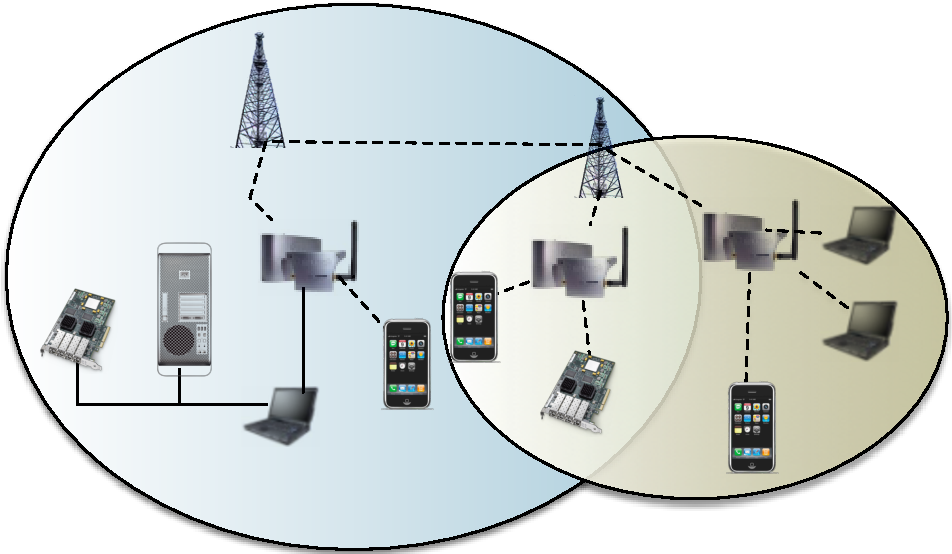
\includegraphics[width=0.6\linewidth]{img/antennes2.pdf}
 	%\vspace{-0.2cm}
 	\caption{Exemple de communautés interconnectées dans une plate-forme multi-échelle}
 	\label{fig:antennes}
 	%\vspace{-0.5cm}
 \end{figure}

\subsection{Optimisations pour le \textit{big data}}
%
Dans le cadre du traitement de données issus des dispositifs de l'IoT, un autre facteur à prendre en compte est celui de la performance liée à l'accès et à la gestion des données. En effet, la plupart des opérations impliquent la collecte, la transformation et l'analyse des données, et les plates-formes telles que Apache Hadoop se sont illustrées par leur capacité d'optimiser l'accès aux données en plaçant les tâches préférentiellement là où les données sont présentes (grâce au concept de la \textit{data locality}). 

Dans le passé \cite{Steffenel2015Roma} nous avons déjà mené des expérimentations avec CloudFIT démontrant que des performances similaires ou supérieures à celles de Apache Hadoop pourraient être atteintes avec un système P2P, comme illustré en Figure \ref{fig:Hadoop}. Bien que ces résultats aient été positifs, nous avons observé deux points qui pourraient être encore améliorés : la surcharge de gestion des données sur un n{\oe}ud et la prise en charge de la \textit{data locality}. 

\begin{figure}[!ht]
	%\renewcommand{\figurename}{Figura}
	\centering
	%\vspace{-0.3cm}
	\includegraphics[width=0.65\linewidth]{img/CloudFIT-mesures.pdf}
	%\vspace{-0.2cm}
	\caption{Comparaison des temps d'exécution de WordCount avec CloudFIT et Hadoop}
	\label{fig:Hadoop}
	%\vspace{-0.2cm}
\end{figure}

Dans le premier cas, nous avons constaté un fort écart de performances d'accès aux données lorsque nous déployons CloudFIT  dans un environnement hétérogène. Ces écarts de performance sont en effet une combinaison de la vitesse d'accès aux données et de la surcharge de gestion des systèmes de stockage (voir aussi les limitations physiques de stockage), et affectent notamment les dispositifs de faible capacité. Ainsi, par exemple, un Raspberry Pi est fortement pénalisé par la vitesse et la capacité de stockage de sa carte SD, malgré une capacité de calcul suffisante (notamment en utilisant tous ses c{\oe}urs de calcul).  

Afin de contourner cette limitation, nous avons modifié la couche de stockage de manière à ce que les n{\oe}uds puissent choisir d'agir seulement en tant que clients distants. Ces n{\oe}uds peuvent donc interroger le service de stockage DHT via le réseau mais ils ne sont plus obligés à gérer le stockage, réduisant leur surcharge et aussi leur utilisation du disque.

Pour ce qui est de la prise en charge de la \textit{data-locality}, cela est un problème plus général qui affecte la plupart des architectures de stockage P2P. En effet, les API de stockage P2P sont souvent basés sur les tables de hachage distribuées (DHT). Ces DHTs sont conçues de manière à répartir les données sur le réseau et les répliquer lorsque cela est possible, notamment afin d'éviter la perte de données en cas de désabonnement (\textit{churn}). Un inconvénient de cette procédure est qu'on observe une perte d'information concernant la localisation des données \cite{Wu2005}, rendant difficile l'optimisation des transferts réseau. Nous avons donc développé deux mécanismes distincts visant à contourner cette limitation. 

La première approche que nous avons développée peut facilement être mise à l'{\oe}uvre si on un accès à la bibliothèque DHT. Cette stratégie consiste à instruire l'ordonnanceur de tâches (\textit{TaskScheduler}) à vérifier préalablement quelles tâches seraient favorisées par la présence des données dans son cache DHT local. Même si c'est une opération de bas niveau, la plupart des DHT P2P offrent la possibilité d'effectuer un \textit{lookup} pour savoir si la ressource requise se trouve déjà dans le cache local ou s'il faut la chercher sur le réseau. En donnant la priorité aux tâches qui peuvent travailler avec des données locales, on peut espérer augmenter la performance globale de l'exécution.

Toutefois, il n'est pas toujours possible d'avoir des données en local dans un overlay P2P. En effet, dans une DHT les n{\oe}uds responsables par le stockage et indexation des ressources sont définis par la clé de hachage de la ressource. La Figure \ref{fig:pastry} illustre le cas du routage d'un message dans l'overlay Pastry \cite{Pastry01, Castro2002}, mais le même exemple peut être utilisé pour la localisation des ressources dans la DHT PAST \cite{Rowstron2001b} car dans ce système les clés des ressources et les clés des n{\oe}uds se superposent. Finalement, même avec de la réplication, il y a le risque que dans un grand réseau les ressources ne se trouvent sur aucun des n{\oe}uds de calcul. Ceci nous amène à l'élaboration d'une stratégie pour renforcer la proximité des données, grâce à un calcul personnalisé de la clé de localisation des ressources. 


\begin{figure}[!ht]
	%\renewcommand{\figurename}{Figura}
	\centering
	%\vspace{-0.3cm}
	\includegraphics[width=0.4\linewidth]{img/AnneauPastry.pdf}
	%\vspace{-0.2cm}
	\caption{Exemple de routage d'un message dans l'overlay Pastry \cite{Castro2002}}
	\label{fig:pastry}
	%\vspace{-0.2cm}
\end{figure}


Cette technique a été élaborée sur la base des spécificités de la DHT de TomP2P, et donc ne peut pas être facilement généralisée. Contrairement à la plupart des systèmes de P2P qui ont seulement une clé de hachage, TomP2P identifie les ressources par quatre clés différentes $\{k_l,k_d,k_c,k_v\}$, selon la hiérarchie suivante : 
\begin{itemize}
	\item \textit{$k_l$} - clé de localisation, utilisée pour la localisation d'une ressource dans la DHT ;
	\item \textit{$k_d$} - clé de domaine, fonctionne comme une clé d'authentification, permet la séparation des données ;
	\item \textit{$k_c$} - clé de contenu, permet d'identifier une ressource. Par défaut celle-ci est identique à la clé de localisation ;
	\item \textit{$k_v$} - clé de version, permet la gestion de versions multiples d'une ressource.
\end{itemize} 

La clé de localisation est celle qui s'approche le plus des clés DHT traditionnelles, ayant par fonction l'association d'une ressource (copie primaire ou index) au n{\oe}ud avec l'ID le plus proche. Sans aucune instruction supplémentaire, la clé de localisation et la clé de contenu sont les mêmes, mais peuvent être différentes par exemple pour résoudre les cas de collision de clés (deux ressources générant la même clé de localisation).

La clé de domaine est liée à un mécanisme d'authentification simple de TomP2P, son but étant de renforcer le cloisonnement des données des différents clients (cette authentification peut être renforcée par l'utilisation de la cryptographie afin de garantir une véritable confidentialité). Dans le cas de CloudFIT, la clé de domaine est utilisée comme un \textit{namespace} pour la séparation des données de différents communautés ou jobs de calcul. 

Finalement, la clé de version permet la coexistence de différentes versions d'une ressource, ce qui permet une meilleure gestion des données "mutables", avec par exemple un accès à l'historique des modifications ou l'écriture en parallèle d'une ressource par plusieurs n{\oe}uds. Cette clé de version est utilisée dans les nouvelles versions de l'application \textit{MapReduce} développée sur CloudFIT.

Ainsi, afin de renforcer la \textit{data locality}, nous avons travaillé sur le découplage entre la clé de localisation et la clé de contenu grâce à une double fonction de hachage. Dans un premier moment, la clé de contenu est obtenue avec une méthode de hachage classique. Ensuite, la clé de localisation est calculée en faisant une association limitée aux ID des n{\oe}uds d'une communauté. La Figure \ref{fig:hash} montre l'exemple de cette cartographie en calculant la clé de localisation d'une ressource $r_3$ par rapport à une communauté $Comm_1$.

\begin{figure}[!ht]
	%\renewcommand{\figurename}{Figura}
	\centering
	%\vspace{-0.3cm}
	\includegraphics[width=0.5\linewidth]{img/hashing.pdf}
	%\vspace{-0.2cm}
	\caption{Cartographie des ressources renforçant la data-locality}
	\label{fig:hash}
	%\vspace{-0.2cm}
\end{figure}

Comme la clé de localisation se trouvera parmi les n{\oe}uds de la communauté, on augmente la probabilité de trouver la copie primaire dans les n{\}oe}uds concernés. De plus, cette stratégie n'empêche pas la réplication des données sur d'autres n{\oe}uds, garantissant la persistance des données en cas de défaillances. Cette approche est aussi tolérante aux variations du nombre de membres de la communauté : en cas de disparition d'un n{\oe}ud, c'est une réplique qui prend le relais ; en cas d'un nouveau membre, celui-ci sera intégré à la fonction de hachage normalement.   

\section{Exemples d'Utilisation de CloudFIT}

En tant que plate-forme expérimentale pour le calcul distribué et le \textit{fog computing}, CloudFIT est en constante évolution. Cela n'empêche pas son utilisation comme plate-forme de calcul dans certains de nos projets, notamment ceux dont l'objectif est d'utiliser des réseaux avec des éléments volatiles ou avec des ressources hétérogènes. Le premier exemple ci-dessous illustre une utilisation "recherche" pour le projet STIC-AmSud PER-MARE, dans le but d'évaluer le comportement de CloudFIT en tant que plate-forme \textit{MapReduce} pour les environnements pervasifs. Le deuxième exemple démontre une utilisation "production", où CloudFIT a été utilisé pour exécuter un workflow destiné aux sciences de l'atmosphère. Ce dernier travail a servi de base  pour la proposition du projet de collaboration CAPES-Cofecub MESO. 


\subsection{L'application WordCount}

Le projet STIC-AmSud PER-MARE (\textit{Adaptive Deployment of MapReduce-based Applications over Pervasive and Desktop Grid Infrastructures}) avait pour but le développement de stratégies pour le déploiement d'applications \textit{MapReduce} sur des environnements pervasifs. Si l'un des volets du projet a été celui d'adapter Apache Hadoop (voir la Section \ref{sec:Guilherme}), l'autre volet consistait à utiliser CloudFIT en tant que plate-forme de calcul distribuée. Si dans l'article présenté à CLIoT 2015 \cite{Steffenel15Taormina} nous nous sommes concentrés sur la performance de CloudFIT (voir aussi la Figure \ref{fig:Hadoop}), le travail présenté à CN4IoT \cite{Steffenel2015Roma} analysait l'exécution de CloudFIT par rapport à la volatilité et l'hétérogénéité des ressources.

\subsubsection{Impact de la volatilité}

Cette première expérience illustre le déploiement d'une application \textit{MapReduce} simple (\texttt{WordCount}) sur un corpus de textes faisant 1 GB de données et réparti en blocs uniformes de 64 MB. Cette répartition vise à reproduire le comportement de Hadoop, qui lui aussi traite les données par blocs de 64 MB.  Aussi afin de rendre la visualisation des expériences plus simple, les n{\oe}uds sont identiques et ont été explicitement limités à une seule exécution simultanée (un seul \texttt{Worker}). 

Dans un premier moment et afin d'avoir un barème de comparaison, la Figure \ref{fig:regular} présente le diagramme de Gantt pour une exécution sans incidents.
Nous pouvons avoir un aperçu du mécanisme d'ordonnancement distribué par défaut de CloudFIT, déjà discuté en Section \ref{subsec:commCloudFIT}. En effet, lorsque la liste de tâches est reçue par le TaskScheduler, celle-ci est réordonnée de manière aléatoire. L'ordonnanceur choisit ainsi la première tâche disponible (marquée "\textit{NEW}") et avertit les autres n{\oe}uds que cette tâche est en exécution. De manière similaire, à la fin de son exécution son statut est diffusé pour annoncer la fin de la tâche. Si toutes les tâches "\textit{NEW}" ont déjà été prises, un n{\oe}ud peut lancer des tâches spéculatives parmi celles marquées "\textit{STARTED\_DISTANT}". 

Plus spécifiquement, nous pouvons observer le déploiement des tâches \textit{map} (lesquelles ont des temps d'exécution variable selon le nombre de mots dans les documents), plus une tâche \textit{reduce} qui s'exécute à la fin. Bien que l'exemple \texttt{WordCount} ne contienne qu'une tâche Reduce, celle-ci se trouve exécutée par tous les n{\oe}uds car si le premier n{\oe}ud a marqué la tâche comme "\textit{STARTED}" et prévient les autres, ceux-ci n'ont rien de plus dans leur file d'exécution et lancent le Reduce en tant que tâche spéculative. Ceci n'a aucun impact sur le résultat final de l'application car les n{\oe}uds vérifient la présence d'un fichier de sortie avant de l'écrire sur la DHT, empêchant tout écrasement ou corruption. 

\begin{figure}
	\centering
		\includegraphics[width=1\linewidth]{img/regular2}
		\caption{Exécution de WordCount sur un cluster uniforme (1 GB de données en blocs de 64MB)}\label{fig:regular}
\end{figure}




Grâce à ces échanges, il est aussi possible de compléter les tâches initiées par les n{\oe}uds en défaillance ou mettre au courant un n{\oe}ud qui vient de rejoindre une communauté CloudFIT. La Figure \ref{fig:1out} représente ainsi une situation où un n{\oe}ud tombe en panne, avec la subséquente reprise des tâches par les autres n{\oe}uds. La Figure \ref{fig:reprise} va au-delà de cette situation en rajoutant un nouveau n{\oe}ud, qui récupère l'état actuel des tâches et peut ainsi contribuer avec l'effort de calcul.
\begin{figure}
	\centering
		\includegraphics[width=1\linewidth]{img/1out2}
		\caption{Exécution de WordCount lorsqu'un n{\oe}ud disparaît (1 GB de données en blocs de 64MB)}\label{fig:1out}
\end{figure}

\begin{figure}
	\centering
		\includegraphics[width=1\linewidth]{img/reprise2}
		\caption{Exécution de Wordcount lorsqu'un n{\oe}ud rejoint la communauté après la défaillance d'un autre n{\oe}ud (1 GB de données en blocs de 64MB)}\label{fig:reprise}
\end{figure}


\subsubsection{Impact de l'hétérogénéité}

Cette deuxième expérience vise l'observation de CloudFIT dans un environnement hétérogène. Pour cela, nous avons interconnecté quatre n{\oe}uds avec des spécifications assez différentes (cf. le Tableau \ref{Table:laptops}). Comme dans l'expérience précédente, nous limitons le nombre de c{\oe}urs (\texttt{Workers}) sur les machines pour rendre la visualisation plus simple.

\begin{table}
	\begin{center}
		\begin{tabular}{|c|c|c|c|c|c|c|}
			\hline
			Type de N{\oe}ud & Processeur & GHz &  Mémoire & OS\\
			\hline
			\hline
			MacBook Air & Intel Core i7-4650U & 1.7   & 8 GB & MacOS 10.10.5 \\
			Lenovo U110 & Intel Core2 Duo L7500 & 1.6   & 4 GB & Ubuntu Linux 15.4 \\
			Raspberry Pi 2 & ARM Cortex-A7 & 0.9  & 1 GB & Raspbian Linux Wheezy\\
			VM Virtualbox & Intel Core i7* & 2.2*  &  1 GB & Debian Linux 8.2 \\
			\hline
			\multicolumn{5}{l}{* ces valeurs sont celles vues par la machine virtuelle}
		\end{tabular}
	\end{center}
	\caption{\label{Table:laptops}Spécification des n{\oe}uds du cluster pervasif}
\end{table} 

Nous avons aussi modifié les paramètres de l'expérience afin d'exécuter le WordCount sur 512MB de données divisées en petits blocs de 2MB seulement ; nous pensons que cette configuration est plus proche de celle rencontrée lors de la transmission de données par les dispositifs IoT. La multiplication de tâches avec un coût individuel plus réduit rend aussi possible la participation des n{\oe}uds avec moins de puissance de calcul.  La Figure \ref{fig:hetero} affiche le diagramme de Gantt pour une exécution de ce scénario. 

\begin{figure}
	\centering
		\includegraphics[width=1\linewidth]{img/hetero2}
		\caption{Exécution de Wordcount dans un cluster hétérogène (512MB en blocs de 2MB)}\label{fig:hetero}
\end{figure}

Alors que la répartition des tâches entre les notebooks et la machine virtuelle ne présentent pas une différence significative, le Raspberry Pi, sans surprise, n'arrive pas à exécuter les tâches aussi vite que les autres n{\oe}uds (voir la longueur des tâches dans la première partie de l'exécution). De plus, ce n{\oe}ud est tellement surchargé qu'il perd plusieurs messages de mise à jour et ne détecte pas la fin de la phase \textit{map}. Comme résultat, il essaye vainement d'exécuter toutes les tâches juste pour se rendre compte que leur résultat est déjà dans la DHT, la raison pour la petite durée des tâches vers la fin (cette vérification préalable était prévue pour éviter le travail en doublon et les risques de corruption des données). 

Au lieu de freiner notre intérêt par les dispositifs de faible puissance, ces résultats nous incitent à vouloir comprendre les raisons de ces problèmes. En effet, les dispositifs de faible puissance tels que les Raspberry Pi n'ont pas seulement des processeurs moins rapides mais aussi des limitations sur la taille et la vitesse d'accès à la mémoire et au stockage (quelques centaines de MB de RAM, des mémoires SD à la place des disques durs, etc.). Dans ces dispositifs, les tâches de gestion de l'overlay P2P et de la DHT (par exemple, la réplication des données) peuvent occuper une partie importante de leurs ressources et finir par interférer avec le traitement des messages échangé via l'overlay.  Ces résultats ont motivé la mise en place des stratégies de collecte de contexte pour un meilleur ordonnancement et aussi les méthodes d'optimisation du stockage que nous avons détaillé dans la section précédente. 

\subsection{Détection d'Événements Secondaires de la Couche d'Ozone}

La découverte du trou d'Ozone de l'Antarctique \cite{Farman1985} a galvanisé l'intérêt de la communauté scientifique et depuis ce moment plusieurs études ont été menées dans le but de surveiller la variation de la densité de la couche d'Ozone sur les régions polaires \cite{Solomon1999}\cite{Salby2012}. La réduction de la couche d'Ozone peut aussi déclencher plusieurs événements sur des zones situées à des latitudes moyennes, soit à cause du mouvement de la bordure du vortex polaire sur ces régions  \cite{Kirchhoff1997}\cite{Marchand2005} ou bien à cause du transit de masses d'air pauvres en Ozone détachées du vortex polaire. Ce dernier cas est appelé "événements dus à l'influence du trou d'ozone Antarctique", ou plus simplement des Événements Secondaires de l'Ozone" (\textit{Ozone Secondary Events}  - OSE). 

Causés par la circulation de l'atmosphère, ces masses d'air continuent à se déplacer pendant 7 à 20 jours après leur séparation du vortex polaire et peuvent atteindre des latitudes plus élevées, occasionnant une réduction temporaire de la colonne totale d'Ozone (\textit{Total Column Ozone} - TCO) sur des zones qui sont souvent habitées \cite{Prather1990}\cite{Waugh1994}\cite{Manney1994}. Comme résultat, des niveaux élevés de radiation ultraviolet nocive (UVB et UVC) atteigne la surface \cite{Casiccia2008}, à un tel point qu'une réduction de 1\% de la colonne totale d'Ozone peut occasionner une augmentation de 1.2\% de la radiation UV mesurée sur le sud du Brésil \cite{Guarnieri2004}. Ces événements secondaires de l'Ozone sont régulièrement observés sur des zones peuplés en moyenne latitude, comme par exemple en Amérique du Sud \cite{Kirschhoff1996}\cite{Pinheiro2011}, en Afrique du Sud \cite{Semane2006}\cite{Sivakumar2007}, à la Nouvelle Zélande \cite{Brinksma1998} et aussi sur l'Île de la Réunion \cite{toihir2015}. 

%\begin{figure}
%	\centering
%	\includegraphics[width=0.75\linewidth]{img/22_10_13-c}
%	\vspace{-0.2cm}
%	\caption{OMI satellite image for 18 October 2013 (a) and the associated wind currents for (b) 19 and (c) 22 October 2013 at 620K}
%	\label{fig:event2013}
%	\vspace{-0.3cm}
%\end{figure}

Malgré une forte liaison avec la dynamique de la stratosphère, le nombre d'études visant la modélisation de la circulation dynamique de la couche d'Ozone sont encore très rares \cite{Marchand2005}. En effet, la plupart des modèles climatiques se limitent aux couches inférieures de l'atmosphère, notamment celles liées à aux prévisions météorologiques, et n'explorent pas les interactions avec les couches supérieures comme celle où se trouve la couche d'Ozone. Plus récemment, un modèle obtenu par Vaz Peres \cite{Peres2013} a permis une certaine compréhension de ces phénomènes. En se concentrant sur les données d'épisodes OSE déjà identifiés dans le passé, le modèle de Vaz Peres a permis la reproduction des événements observés. En partant de cette étude, notre but était d'utiliser des techniques du \textit{big data} et du \textit{data mining} afin de ramasser plus de données et extraire des modèles plus précis, permettant la prévision des occurrences de ces événements.

L'utilisation de techniques du \textit{big data} est essentiel car les données concernant la couche d'Ozone s'accumulent d'année en année. Par exemple, l'équipement TOMS/OMI placé dans les satellites de la NASA satellite produit plus d'1GB de données brutes par an. Juste les observations des satellites TOMS/OMI remontent à 1978 (ce qui fait presque 40 GB en ce moment), et à cela on peut rajouter d'autres sources de données satellites telles que les satellites de l'ESA mais aussi des observations effectuées au sol. 

\subsubsection{Identification des événements secondaires de l'Ozone avec CloudFIT\label{sec:development}}

Si dans un premier temps l'usage d'une plate-forme type cluster ou cloud pourrait être envisagée, notre attention s'est portée sur CloudFIT car celui-ci a l'avantage d'exploiter les ressources de calcul disponibles, sans obliger l'installation ou la maintenance d'un parc informatique dédié. En autre, le traitement des données et la détection des OSE varie selon la zone géographique couverte et selon le type d'analyse effectuée : la détection d'événements passés utilisée pour améliorer les modèles est assez simple, alors qu'une analyse plus poussée visant l'étude des corrélations entre les événements et les courants atmosphériques peut s'avérer bien plus demandeuse de ressources. L'utilisation de CloudFIT permet la création d'une plate-forme de calcul élastique.

Dans le cas précis de la détection des OSE, nous avons identifié quatre activités principales qui peuvent être transposées sur CloudFIT. Ces activités sont les suivantes : 
\begin{enumerate}
	\item \textbf{Pré-traitement des données} - transformation des données brutes OMI ;
	\item \textbf{Filtrage et agrégation} - sélection des données concernant une zone géographique et une période donnée, puis des opérations d'agrégation si nécessaire ;
	\item \textbf{Extraction des paramètres} - extraction des moyennes et écarts types pour une région et une période donnée ;
	\item \textbf{Détection des événements} - identification des valeurs anormales d'Ozone, génération d'alertes.
\end{enumerate}

Le pré-traitement des données est nécessaire car les données brutes fournis par l'équipement TOMS/OMI sont dans un format difficile à utiliser. Le filtrage permet de limiter la recherche sur une zone géographique et/ou sur une période d'étude, alors que l'agrégation permet l'obtention de données à une granularité différente de celle d'origine (utile notamment pour la corrélation avec d'autres types de données). En effet, la plupart des données TOMS/OMI ont une résolution d'1 dégrée, alors que d'autres sources de données ont parfois des cartographies plus détaillées (par exemple, avec 0.25 dégrée d'arc entre chaque mesure). Cette procédure sera détaillée dans la section suivante.

L'extraction des paramètres est la prochaine étape car la détection d'un OSE est liée à l'observation d'une chute anormale de la concentration de l'Ozone. Pour cela, il faut extraire des paramètres historiques tels que la moyenne et la variation (écart-type), et cela pour chaque coordonnée analysée. Cette procédure est aussi détaillée dans les sections suivantes. Finalement, la détection se fait en comparant la mesure d'un instant précis avec la série temporelle des journées précédentes. Si les valeurs sont inférieures à la variation normale de la période, alors on peut déclencher une procédure d'alerte, signalant aux autorités sanitaires un risque lié à la radiation UV qui menace la population.

Les trois premières activités sont des exemples d'opérations ETL (\textit{Extract, Transform, Load}) typiques du \textit{big data}. La dernière activité peut être considérée comme un algorithme de prise de décisions. Nous avons donc établi un workflow qui peut être transcrit comme un enchaînement de jobs CloudFIT, comme illustré en Figure \ref{fig:blocs}. Par conséquent, les quatre premiers jobs (Preprocess, Filtering, Time-series et Detection) peuvent même être exécutés sur des communautés CloudFIT différentes : des équipements entrée de gamme regroupés en Community C1 peuvent être utilisés pour pré-traiter et stocker les données des satellites et des spectre-photomètres Brewer ou Dobson installés au sol. 

Par la suite, les données peuvent donc être traitées pour la détection ou bien être utilisées pour des analyses plus poussées telles que la recherche de motifs récurrents ou la prévision d'événements futurs. Les activités telles que le filtrage et l'analyse des séries temporelles demandent des ressources de calcul plus importants, fournis par la communauté C2.
La Figure \ref{fig:blocs} inclut aussi d'autres communautés (C3 et C4) qui pourraient être déployées séparément afin d'effectuer les autres activités liées à la détection et à la prévision des OSE (ces étapes n'ont pas été implémentées). Il faut noter que cette organisation répond aussi aux principes du calcul multi-échelle et du \textit{fog computing}, l'un des objectifs de CloudFIT.

\begin{figure}
	\centering
	\includegraphics[width=1\linewidth]{img/4-process}
	\caption{Organisation des activités dans un réseau CloudFIT}\label{fig:blocs}
\end{figure}

\subsubsection{Pré-traitement des données}

Les mesures de la colonne totale d'ozone peuvent être obtenues par des équipements au sol mais aussi par le biais des satellites, qui ont l'avantage d'offrir une couverture globale. L'un de ces équipements, l'instrument TOMS/OMI, rend publique les données consolidées de la couverture du globe, une fois par jour. Dans le cas de la détection des événements secondaires de l'Ozone, nous avons besoin des données brutes obtenus par les satellites. Ces données sont présentées selon le format illustré en Figure \ref{fig:toms}(a), ce qui n'est pas vraiment adapté à l'utilisation direct pour nos calculs. Chaque fichier contient un entête avec des informations sur le fichier (date, les coordonnées du grillage, le pas), suivi des mesures pour chaque latitude (indiquée à la fin de la ligne), et cela pour toutes les longitudes couvertes. Chaque mesure est exprimée en unités Dobson (UD), représentées par un entier à 3 chiffres qui doit être séparé des mesures des autres longitudes. Par exemple, les coordonnées (-89.5,-179.5) de la Figure \ref{fig:toms}(a) ont la valeur 280, les coordonnées (-89.5,-178.5) ont aussi la valeur 280, et ainsi de suite.   

\begin{myverbbox}[\tiny]{\TOMS}
	Day:   1 Jan  1, 2013    OMI TO3    STD OZONE    GEN:13:003 Asc LECT: 01:44 pm 
	Longitudes:  360 bins centered on 179.5  W  to 179.5  E   (1.00 degree steps)
	Latitudes :  180 bins centered on  89.5  S  to  89.5  N   (1.00 degree steps)
	280280280280280280280280280280280280280280280280280280280279279279279279279
	279279279279279279279279279279279279279279279279279279279279279279279279279
	279279279279279279279279279279279279279279279279279279279279279279279279279
	279279279279279279279279279279279279279279279279279279280279280280280280280
	280280280280280280280280280280280280280280280280280280280280280280280280280
	280280280280280280280280280280280280280281281281281281281281281281281281281
	(...)
	282282282282282282282282282282   lat =  -89.5
	(...)   lat =  -88.5
	(...)   lat =  -87.5
	(...)
\end{myverbbox}

\begin{myverbbox}[\tiny]{\JSON}
	{
		"date":"20130101",
		"step":"1.0",
		"latitudes":{
			"-89.5":["-179.5":"280","-178.5":"280",(...)],
			"-88.5":["-179.5":"272","-178.5":"272",(...)],
			(...)
		}
	}
\end{myverbbox}

\begin{figure}
	\centering
	\begin{tabular}{cc}
		\imagetop{\TOMS}&\imagetop{\JSON}\\
		{\small (a)}&{\small (b)}
	\end{tabular}
	%\vspace{-0.2cm}
	\caption{Fichier brute OMI Ozone (a) et sa représentation JSON (b)}\label{fig:toms}
	%\vspace{-0.3cm}
	
\end{figure}

Comme ce format est difficile à comprendre et à traiter (il faut parcourir l'ensemble des entrées d'une latitude pour obtenir une mesure à une longitude donnée), nous avons décidé de pré-traiter ces fichiers et les stocker sur la DHT en tant que objets JSON, selon le \textit{template} présenté en Figure \ref{fig:toms}(b). JSON est un format structuré de données bien connu, qui peut être facilement requêté, importé sur des bases de données ou bien stocké directement dans des bases NoSQL orientées  documents. Le pré-traitement est facilement parallélisable car chaque journée peut être traitée indépendamment des autres. De plus, le stockage sur une DHT permet la réutilisation de données déjà traitées et l'ajout de nouvelles entrées à chaque jour. 

\subsubsection{Analyse des séries temporelles et la détection des OSE\label{sec:timeseries}}

Comme indiqué précédemment, les OSE peuvent être détectés par des réductions anormales de la colonne totale d'Ozone alors que cela n'est pas directement lié à l'expansion du trou de la couche d'Ozone Antarctique. Cette détection est faite par la comparaison entre la mesure d'une journée et les moyennes historiques pour cette région. Cependant, le choix de ce qu'on considère la "période historique" a un impact important sur la perception des événements. Pour commencer, on ne peut pas utiliser la moyenne annuelle car la concentration d'Ozone varie saisonnièrement (dans l'hémisphère sud elle est plus basse à l'Automne et plus haute au Printemps). 

L'approche utilisé par Perez \textit{et al. }\cite{Peres2013} considérait la moyenne historique mensuelle, i.e., la moyenne historique de chaque mois des années enregistrées. De cette forme, une mesure effectuée le 2 Octobre et l'autre le 30 Octobre seraient comparées à la moyenne historique du mois d'Octobre. Si cela permet déjà la détection de certains OSE, cette méthode n'est pas suffisamment précise car la concentration naturelle varie d'année en année et aussi parce que la variation entre le début et la fin d'un mois est très importante dans les mois de transition comme Juillet ou Novembre. L'utilisation d'une moyenne standardisée aurait comme conséquence un nombre important de faux-positifs et faux-négatifs. Vu que nous disposons de ressources de calcul, nous avons décidé d'utiliser une approche par fenêtres glissantes, où par exemple chaque mesure est comparée à la moyenne des 15 jours précédents. Cette solution (l'utilisation de \textit{time series}) est plus proche de la réalité et prend en compte la variation naturelle pour la période étudiée.

Comme pour le pré-traitement des fichiers d'entrée, cette activité peut être exécuté en parallèle car chaque coordonnée (X, Y) a son propre ensemble de données. De même, le calcul de la moyenne et de l'écart type est indépendant pour chaque jour choisi, vu que la fenêtre glissante couvre des dates différentes. Ainsi, dans l'implémentation CloudFIT, les tâches de calcul sont définies en fonction du nombre de coordonnées. Chaque tâche lit les valeurs pour les 15 jours précédents et calcule la moyenne et l'écart type. Par exemple, si nous considérons la zone couverte par les coordonnées \{(-70.5, -84.5), (-20.5, -29.5)\} (les mêmes utilisées en Figure \ref{fig:progression}) avec un pas d'1 dégrée pour le grillage, nous avons 50x55 points à analyser (2750 tâches). 

Une fois obtenus la moyenne et l'écart type pour chaque coordonnée et pour chaque jour cible, la détection des OSE peut être effectuée.  Pour cela, nous utilisons la formule simple présentée en Équation \ref{eq:equation}. Cette formule considère qu'un OSE existe si la valeur mesurée est inférieure à un seuil déterminé en fonction de la moyenne des 15 derniers jours et de la latitude (dans le cas du sud du Brésil on considère ce seuil à $1.5 \times$ l'écart type). Des paramètres additionnels tels que la vorticité potentielle pourraient être rajoutés afin d'augmenter la précision des détections.

\begin{equation}
Detection(v)=\left\{ \begin{array}{c}
\begin{array}{lll}
\textbf{True} & &if \:\: v \:< (average - 1.5\times stdev)\\
\textbf{False} & &otherwise\end{array}\end{array}\right.
\label{eq:equation}
\end{equation}



\subsubsection{Résultats préliminaires}

Afin de valider l'implémentation, nous avons comparé les données de Peres \textit{et al.} \cite{Peres2013} avec les résultats obtenus à partir du workflow CloudFIT. Comme attendu, notre implémentation permet d'observer la progression du front OSE entre le 18 et le 22 Octobre 2013 (Figure \ref{fig:progression}). On observe que le mécanisme de détection mis en place permet de se concentrer uniquement sur les zones ayant subi une variation importante de la colonne d'Ozone et pas sur celles qui habituellement ont une concentration réduite (comme par exemple le pôle ou les régions australes de l'Argentine et du Chili). 

\begin{figure}
	\centering
	\includegraphics[width=0.19\linewidth]{img/20131018-b}~\includegraphics[width=0.19\linewidth]{img/20131019-b}~\includegraphics[width=0.19\linewidth]{img/20131020-b}~\includegraphics[width=0.19\linewidth]{img/20131021-b}~\includegraphics[width=0.19\linewidth]{img/20131022-b}
	%\vspace{-0.2cm}
	\caption{Progression de l'OSE observé entre le 18 et le 22 Octobre 2013}\label{fig:progression}
\end{figure}

Nous avons aussi comparé les coordonnées des OSE par rapport aux données de vorticité potentielle, l'un des facteurs étudiés par Peres. Afin de ne pas surcharger l'image, nous avons tracé seulement les points situés à proximité de l'observatoire de Santa Maria (Brésil). Comme montrent les cartes dans la Figure \ref{fig:comparison}, on observe une forte corrélation entre la vorticité potentielle et l'approximation des masses d'air pauvres en Ozone, spécialement sur la carte du 20 Octobre.  On peut aussi observer que ces OSE prennent du temps à se dissiper : même si la vorticité potentielle s'est déplacée, une poche pauvre en Ozone persiste sur une zone habitée deux jours plus tard. Ces résultats encouragent la poursuite de l'étude de la corrélation entre les OSE et la vorticité potentielle.


\begin{figure}
	\centering
	\includegraphics[width=0.75\linewidth]{img/comparison2}
	%\vspace{-0.2cm}
	\caption{Superposition des cartes de la vorticité potentielle et le OSE identifié sur l'observatoire de Santa Maria, Brésil (29.68 S, 53.81 W)}\label{fig:comparison}
\end{figure}

La scalabilité de l'application a aussi été étudiée car cet algorithme peut être utilisé autant pour des détections journalières que pour des analyses plus poussées sur des périodes ou zones plus importantes. Ainsi, par exemple, l'analyse de la période entre le 15 et le 31 Octobre 2013 a été fait dans une cluster pervasif composé de seulement deux machines (un Macbook Air  - Intel i7-4650U, 2 c{\oe}urs, 8GB RAM -  et un Dell Precision T5610 - 2x Intel Xeon E5-2620, 12 c{\oe}urs, 32GB RAM). 

En utilisant l'ensemble des c{\oe}urs de calcul de chaque machine, l'analyse a duré 570 secondes. Ceci peut être optimisé en augmentant le nombre de coordonnées traitées par chaque tâche (cela réduit le surcout du démarrage d'une nouvelle tâche) mais aussi on peut rajouter d'autres n{\oe}uds au cluster pervasif. En comparaison, l'évaluation d'une seule journée avec un Raspberry Pi 2 a nécessité 40 minutes. Malgré sa faible performance, l')usage de dispositifs bas de gamme comme les Raspberry Pi reste une alternative économique et suffisante pour certains types de tâches, comme le pré-traitement et la détection à partir des données journalières. Si par contre nous avons besoin d'explorer un grand ensemble de données historiques, des machines plus puissantes peuvent être allouées à des communautés CloudFIT dédiées à ces tâches plus lourdes. 

\section{Bilan et Perspectives}


\Bigchapter{Conclusion et perspectives}

% !TeX spellcheck = fr_FR

Tout au long de ce document j'ai essayé de mettre en évidence les différentes façons dont l'hétérogénéité peut affecter l'opération d'un système ou d'une application, ainsi que mes contributions pour leur prise en charge.

L'hétérogénéité peut se présenter sous différentes formes, demandant des actions spécifiques selon l'application, l'environnement et le contexte d'utilisation. Une première catégorie représente les \textit{variations matérielles} des composants d'un système informatique. À l'hétérogénéité matérielle s'ajoutent les problèmes de l'\textit{hétérogénéité des communications}, dont la prise en charge se fait notamment par l'optimisation des échanges des messages (Chapitre \ref{chap:grids}), et \textit{l'hétérogénéité des tâches}, résultat d'une distribution déséquilibrée de charge entre les différents ressources participant à un calcul (Chapitre \ref{chap:amide}). 

Il faut également être capable de supporter les variations des ressources tout au long de l'exécution, vu que \textit{l'hétérogénéité issue de la dynamique} (Chapitre \ref{chap:hadoop}) d'un système peut prendre différentes formes telles que le départ ou l'arrivé de ressources ou bien par leur changement d'état ou de capacité. Finalement, \textit{l'hétérogénéité des données} (Chapitre \ref{chap:grappes}) peut aussi impacter le développement d'une application à cause de leur variété et des spécificités d'accès selon les sources : des objets en mémoire, des fichiers, des URIs ou des requêtes distantes (RPC, Web services, etc.). 

Les travaux que j'ai conduit au fil des années touchent une ou plusieurs de ces manifestations de l'hétérogénéité, et dans ce document j'ai voulu montrer des cas représentatifs de ces travaux. Ainsi, au cours de la première partie de ce mémoire, j'ai présenté des algorithmes issus des mes travaux dont l'objectif était la compréhension des facteurs qui impactent les opérations de communication collective dans les \textit{grids}. J'ai pu exploiter ainsi des méthodes de mesure de performance et de découverte de la topologie réseau, et cela dans le but d'optimiser ces opérations mais aussi afin de pouvoir estimer leur performance avec une haute précision. Avec les années, mes travaux de recherche dans ce domaine se sont déportés vers l'analyse de performance des applications et systèmes, mais ayant toujours comme objectif l'optimisation des performances.

Dans la deuxième partie, j'ai utilisé comme exemple les efforts faits pour gérer l'hétérogénéité des tâches lors de la parallélisation et la gestion de l'exécution distribuée d'une application en biochimie. À partir d'une exécution monolithique, j'ai participé au développent de stratégies visant à découper l'espace de données et d'ainsi permettre la création de tâches de calcul pouvant être exécutées en parallèle. Ceci a été accompagné par le développement d'une plateforme de déploiement capable de gérer l'exécution des tâches distribuées sur  un \textit{cluster} HPC ou sur un ensemble de n{\oe}uds volontaires. Bien que relativement simple d'un point de vue technique, les activités développées pendant le co-encadrement de cette thèse m'ont apporté du recul vis-à-vis des processus nécessaires à la parallélisation et au déploiement d'une application tiers.

La troisième partie de ce mémoire se consacre à la dynamique des ressources et aux stratégies pour sa prise en charge. Ceci est illustré par une expérience visant à améliorer le comportement de la plateforme \textit{big data} Apache Hadoop dans les environnements hétérogènes et dynamiques (qu'on nomme ici environnements pervasifs). En s'aidant d'un mécanisme de collecte d'informations sur le contexte des ressources, il a été possible de modifier ce \textit{framework} et ainsi d'adapter la gestion des tâches aux ressources disponibles à chaque instant. Les concepts développés ici ont fortement influencé l'ensemble de mes activités de recherche, qui depuis se sont orientées vers le support à la dynamique des ressources dans les milieux hétérogènes. Ce n'est pas par hasard si mes recherches en ce moment se concentrent sur le \textit{fog computing}.    

La quatrième partie présente la spécification d'une base documentaire permettant l'accès transparent aux sources de données, peu importe leur nature (fichiers, flux, bases de données, etc.). Pour cela, j'ai présenté une spécification pour la construction d'un réseau hiérarchique pouvant héberger cette base documentaire. Les contributions de cette partie sont peut-être moins présentes dans ma recherche du fait d'avoir une préférence sur les réseaux P2P au détriment des réseaux hiérarchiques, toutefois la problématique liée à la diversité des sources de données reste un défi majeur que je fais ressortir notamment dans mes activités d'enseignement.

Finalement, dans la dernière partie de cette habilitation, j'ai présenté en détails la plateforme expérimentale de calcul distribué CloudFIT. Dans un premier moment j'ai montré l'architecture et les mécanismes de communication et de gestion des n{oe}uds, spécifications que jusqu'à présent n'avaient pas été publiées. Par la suite, j'ai introduit les stratégies pour le support à l'ordonnancement adapté au contexte qui font déjà partie de CloudFIT ou qui seront implémentées dans un avenir proche. Cette partie se termine par la présentation de deux exemples d'utilisation de CloudFIT, tous les deux issus de projets internationaux dont j'ai participé. Plus qu'un récapitulatif, ce chapitre a présenté l'évolution de  CloudFIT au fil des années, et son rôle en tant que est devenu une plateforme expérimentale pour mes recherches dans les domaines de l'IoT et du  \textit{fog computing} et l'Internet des Objets (\textit{Internet of Things} - IoT). .

L'ensemble de mes travaux a été à l'origine d'un nombre significatif de publications internationales (11 revues, 37 conférences, 3 posters, 3 chapitres de livre) et nationales (2 revues, 15 conférences, 3 posters). J'ai aussi participé au co-encadrements de deux thèses de doctorat et d'un post-doctorat : la thèse de Romain Vasseur (thèse CIFRE, dirigée par Manuel Dauchez et aussi co-encadrée par Stéphanie Baud), celle de Thierno Ahmadou Diallo (thèse en co-tutelle avec l'Université Cheikh Anta Diop - Sénégal, dirigée par Olivier Flauzac et Samba Ndiaye), et le stage post-doctoral de Iyad Alshabani (dans le cadre du projet ANR USS-SIMGRID). 

J'ai également été en charge de l'élaboration de trois projets de collaboration internationale entre l'Université de Reims et l'Amérique du Sud : le projet STIC-AmSud PER-MARE (2013-2014, avec l'Universidad de la República - Uruguay et l'Universidade Federal de Santa Maria - Brésil), le projet STIC-AmSud CC-SEM (2017-2018, avec L'Universidad de Buenos Aires - Argentine et l'Universidad de la República - Uruguay), puis le projet CAPES-Cofecub MESO (2017-2020, avec l'Université de la Réunion et  l'Universidade Federal de Santa Maria - Brésil). Dans tous ces projets j'ai exercé le rôle de coordinateur pour l'équipe de Reims et, dans le cas du projet PER-MARE, j'ai été aussi le coordinateur international.

Les perspectives associées à mes travaux sont nombreuses, d'une part à cause des projets en cours et d'autre part par les opportunités d'innovation dans les domaines de mes activités. Néanmoins, je souhaite à l'avenir privilégier trois thèmes.

\subsection*{Le \textit{fog computing} et les environnements pervasifs}

Les environnements pervasifs et le \textit{fog computing} constituent pour moi des sujets de recherche prioritaires. Tout d'abord, ils représentent l'opportunité de poursuivre les sujets de recherche auxquels je me suis dédié ces dernières années : la prise en compte de l'hétérogénéité des ressources, de l'hétérogénéité des tâches, de la volatilité, de l'ordonnancement sensible au contexte et du calcul multi-échelle. 

Le grand attractif des environnement pervasifs et \textit{fog computing} reste toutefois la diversité de problèmes ouverts. Le manque de standardisation n'a pas encore permis un consensus entre les chercheurs, résultant en multiples visions qui ne sont pas toujours compatibles. Même si une spécification voit le jour demain, elle sera forcément réductrice et donnera naissance à de nouveaux verrous scientifiques qu'il faudra explorer : une spécification trop orientée "services dans le \textit{edge}" laissera forcément du vide en ce qui concerne la migration de tâches et de micro-services ; des solutions réseaux contrôlées par les opérateurs auront par conséquence la multiplication des recherches autour des réseaux éphémères contrôlés par les applications. 
 
 À mon avis le principal défi à répondre est celui de la perméabilité des frontières entre l'Internet des objets, le \textit{fog computing} et le \textit{cloud}. Une différentiation trop marquée serait rapidement dépassée du fait de la multiplication des dispositifs IoT et de leur montée en performance. Une perméabilité trop importante induirait plus de défis liés à l'hétérogénéité que nécessaire. En fondant mes recherches dans ce thème, j'espère pouvoir apporter ma contribution.
 
Évidemment, les objectifs à court terme incluent ceux décrits dans les chapitres précédents : continuer le développement de la plateforme CloudFIT, poursuivre la recherche sur le support à la virtualisation et aux micro-services dans les nano-ordinateurs, etc. L'arrivée d'une doctorante en cotutelle et d'un post-doctorant à la fin 2017, dans le cadre du projet CAPES-Cofecub MESO, sera aussi l'occasion de tester l'exécution distribuée de modèles atmosphériques spécifiques pour la couche d'Ozone. Ces projets forment donc le socle de base pour mes recherches à plus long terme sur le \textit{fog computing} et les environnements pervasifs.  

\subsection*{L'Internet of Things et les \textit{smart cities}}

L'IoT est sans aucun doute un sujet prioritaire de ma recherche, autant parce que l'IoT représente un domaine où l'hétérogénéité se présente sous toutes ses différentes facettes, mais aussi parce que l'IoT est une cible prioritaire pour la compréhension du \textit{fog computing}. En effet, dans ma vision, le progrès de l'électronique embarquée fera qu'au moins une partie des dispositifs IoT évoluera jusqu'à devenir des véritables n{\oe}uds de calcul. À partir de ce moment, ces n{\oe}uds seront capables d'effectuer une partie des tâches qui aujourd'hui sont transmises au \textit{cloud} ou aux dispositifs à la périphérie des réseaux. Apprendre à contrôler et à orchestrer le calcul sur ces dispositifs marqués par une forte hétérogénéité serait une étape de plus dans la consolidation d'un véritable \textit{fog computing}.

Les recherches en IoT peuvent aussi s'associer à celles sur les \textit{smart cities}. Cette association nous ouvre un volet applicatif très intéressant, non seulement par la possibilité de mettre en pratique des algorithmes mais aussi à cause de leur impact sur notre vie quotidienne. Ce n'est pas par hasard que plusieurs projets que j'intègre sont orientés dans ce sens. Dans le cas du projet STIC-AmSud CC-SEM, l'objectif principal est le développement d’une plateforme intégrée pour la surveillance et le contrôle de la consommation électrique dans les milieux urbains. Ceci implique donc le développement des dispositifs électroniques pour la mesure de la consommation mais aussi la mise en place du réseau de collecte et d'analyse des données. 

On retrouve aussi la thématique des \textit{smart cities} sous le nom \textit{smart agriculture},  l'un des axes prioritaires de l'Université de Reims Champagne-Ardenne. Dans ce cas, je suis engagé dans un projet avec les chercheurs de l'Unité de Recherche Vignes et Vin de Champagne afin de mettre en place un réseau de capteurs déployé au pied des vignes. Ce réseau IoT permettra la surveillance de paramètres tels que l'humidité du sol, la luminosité et la température autour des plantes, données qui seront ensuite analysées, notamment afin de corréler ces données aux apparitions de certaines maladies. 

Une autre opportunité de recherche à court et moyen terme viendra avec le projet ANR autour de la \textit{Green IT} qui sera soumis cette année. Dans ce projet, nous nous intéressons au développement de stratégies d'ordonnancement basés sur le contexte et sur des objectifs de consommation préétablis afin d'aider à la réduction de l'empreinte énergétique des applications. Ces stratégies peuvent donc être appliquées au développement de services et d'applications mobiles, en utilisant par exemple la migration de composants et d'applications à des fins d'économie d'énergie. 

Les recherches sur l'\textit{Internet of Things} et sur les \textit{smart cities} représentent donc des sujets de recherche à forte valorisation à le court terme, avec l'avantage d'être toujours alignés avec mes objectifs principaux à long terme. 

\subsection*{Le calcul distribué et le big data}

Le dernier thème prioritaire de ma recherche concerne le calcul distribué et le \textit{big data}. Pour être plus précis, je considère que ces deux sujets sont de moins en moins dissociés, les avancées dans le domaine du \textit{big data} étant calquées essentiellement sur des plateformes et techniques issues du calcul distribué. De même, la recherche sur le calcul distribué ne peut plus ignorer les couts liés à la gestion et à la transmission des grandes masses de données, un paramètre qui tend à être encore plus décisif dans le cas des environnements hétérogènes tels que le \textit{fog computing}. 

Les outils pour le calcul distribué (dont le \textit{big data}) sont toutefois encore trop dépendants d'infrastructures stables et homogènes. Comme le prouve notre travail sur le framework Hadoop, il est nécessaire de repenser ou, tout au moins, d'adapter les plateformes et frameworks de manière à mieux gérer l'hétérogénéité et la dynamicité des ressources. En effet, je surveille de près d'autres plateformes telles que Apache Storm, vu que ces plateformes peuvent dans certains cas répondre plus efficacement à certaines exigences d'un déploiement \textit{fog computing} ou, au contraire, bénéficier des techniques développées pour CloudFIT.

Cette thématique présente aussi un volet pratique qui peut venir à supporter mes recherches futures. En effet, la 2\up{ème} phase du projet STIC-AmSud CC-SEM, dédié à la consommation électrique, doit s'élargir afin d'inclure des éléments de traitement \textit{big data} et d'apprentissage automatique (\textit{deep learning}). Le projet CAPES-Cofecub MESO, de son côté, dépend de l'analyse de données afin de comprendre les phénomènes atmosphériques et créer des modèles de prédiction fiables. Afin de remplir ces tâches, je compte autant sur l'expertise des membres de mon équipe sur le \textit{deep learning} que sur l'expérience obtenue pendant mes interventions dans le module "Outils Big Data", lequel j'enseigne aux étudiants en Master 2 Informatique et en Master 2 Statistique pour l'Évaluation et Prospective. 

 En perfectionnant mes connaissances sur les outils et les algorithmes de traitement des données, j'espère bien élargir les possibilités de mes recherches futures, tout en contribuant au développement des thématiques telles que le \textit{fog computing }qui est au centre de mes intérêts.
%
%
%\subsection*{Efficacité énergétique dans le cadre des \textit{Smart cities} et de l'informatique mobile}
%
%L'efficacité énergétique est une thématique forte ces dernières années, avec beaucoup de contribution autant du côté des équipements comme celui des réseaux de distribution mais aussi dans le domaine des \textit{smart cities}. En rejoignant le projet STIC-AmSud CC-SEM, j'ai pu constater que le domaine des \textit{smart cities} est à l'intersection de plusieurs disciplines avec qui j'ai souvent pu travailler : les systèmes distribués, l'IoT et les réseaux de capteurs, les algorithmes de récupération et de traitement de données, etc. De par ma participation à ce projet, les perspectives de recherche à court et moyen terme sont nombreuses.
%
%
%
%
%
%
%\subsection*{Expérimentation et développement de \textit{middlewares} pour le \textit{fog \\ computing}}
%
%Les problèmes de recherche autour du \textit{fog computing} et des environnements pervasifs en général sont multiples. 
%
%Le développement de la plateforme CloudFIT offre à la fois un outil pour la recherche et un cadre pour l'expérimentation de nouvelles techniques. Tout naturellement, je souhaite continuer son développement, intégrant des éléments issus de mes recherches autour du \textit{fog computing} mais aussi autour des projets que je participe. Comme indiqué dans le chapitre dédié à CloudFIT, cette plateforme offre plusieurs outils nécessaires pour la création d'une organisation multi-échelle du réseau, ce que permettrait une meilleure gestion des ressources. La mise en place de mécanismes pour la création à la volée de communautés CloudFIT fait partie de mes priorités immédiates, tout comme le prototypage de la technique de renforcement de la localité des données proposé dans le même chapitre.
%
%Plus à moyen terme, j'envisage rajouter des mécanismes pour la migration des tâches, ce qui permettrait l'expérimentation de stratégies spécifiques pour la distribution des tâches. Les verrous scientifiques dans ce domaine sont nombreux car la migration doit être précédée par une étude des application et des techniques pour garder leur cohésion malgré la migration entre les ressources. Ainsi, par exemple, on pourrait faire usage de machines virtuelles de type conteneur, le moyen le plus simple à mon avis pour effectuer la migration de tâches en exécution. D'autres pistes à suivre concerneraient l'usage de micro-services ou bien une combinaison entre ces deux techniques. Cette activité intégrera probablement les le cadre de la collaboration avec l'Université Paris 1 autour du déploiement de conteneurs sur des nano-ordinateurs. 
%
%
%
%Mon intérêt pour cette thématique ne se limite pas à CloudFIT. En effet, je surveille de près d'autres plateformes telles que Apache Storm, vu que ces plateformes peuvent dans certains cas répondre plus efficacement à certaines exigences d'un déploiement \textit{fog computing}. L'expérimentation et le développement sur ces plateformes permet donc d'obtenir des éléments de comparaison pour CloudFIT et de mieux avancer dans mes recherches dans ce domaine.
%
%
%
%\subsection*{Applications de l'\textit{Internet of Things} et des réseaux de capteurs}
%
%Au delà du développement de \textit{middlwares} pour le \textit{fog computing}, je souhaite continuer à développer des équipements et des outils pour l'IoT, notamment dans le cadre de l'axe "\textit{smart agriculture}" promu par l'Université de Reims Champagne-Ardenne. Ainsi, nous sommes, par exemple, en négociation avec les chercheurs de l'Unité de Recherche Vignes et Vin de Champagne afin de développer un réseau de capteurs (équipement, réseaux et outils) pouvant être déployé au pied des vignes, permettant ainsi de surveiller des paramètres tels que l'humidité du sol mais aussi la luminosité, la température et l'humidité de l'air autour des plantes. D'autre part, nous souhaitons aussi développer des techniques d'analyse de ces données afin de connaître le stress hydrique des plantes et de les corréler avec l'apparition de certaines maladies. 
%
%Je souhaite aussi compléter le développement et le déploiement des micro-contrôleurs Arduino équipés du capteur UV de la gamme ML8511, afin de les intégrer à un réseau de surveillance de l'Ozone Antarctique piloté par CloudFIT. Inséré dans le cadre du projet CAPES-Cofecub MESO, ce réseau sera utilisé en complément des mesures effectuées par des instruments spécifiques tels que les spectre-photomètres Dobson et Brewer. Après une première phase de calibration et tests de durabilité (ces capteurs seront déployés à l'air libre), nous espérons pouvoir disseminer  ces capteurs sur une large zone géographique et ainsi améliorer de manière peu onéreuse la couverture des équipements actuelles.
%
%
% 
%
%%TODO mettre ça dans les conclusions finales ? 
%
%%
%%
%%Ainsi, au cours des travaux antérieurs à ma thèse je m'étais penché sur la détection des pannes et leur impact sur les algorithmes de Consensus, ce qui m'a permis entre-autre de faire un séjour à l'EPFL à Lausanne pour travailler avec le professeur André Schiper. Bien que mes recherches se sont diversifiées au fil des années, c'est une thématique qui revient ponctuellement dans mes travaux, comme dans le cas de l'étude sur la diffusion avec ordre total (REFF).
%%
%%Pendant ma thèse les travaux se sont concentrés sur la modélisation des performances des communications à grande échelle, en profitant de l'essor des recherches sur le grid computing et le lancement du réseau Grid'5000. Cette thématique m'a permis de tisser d'importantes collaborations qui ont perduré après la thèse, comme l'attestent les travaux XXXX et YYY.
%%
%%L'arrivée à Reims marque un tournant dans mes recherches, du fait d'être intégré à une équipe spécialisée dans le calcul distribué et HPC. Tout en poursuivant une partie des travaux sur la modélisation des performances, j'ai été peu à peu  
%%
%%
%%
%%Bien sûr, ce travail n'a pas été le seul dans ce domaine. 
%%	

\Bigchapter{Publications personnelles}

\section*{Articles dans des revues avec comité de lecture}

\subsection*{Internationales}

Steffenel, L.A., Kirsch-Pinheiro, M., Vaz Peres, L., Kirsch Pinheiro, D. "Strategies to implement Edge Computing in a P2P Pervasive Grid", International Journal of Information Technologies and Systems Approach (IJITSA), IGI Global, (accepted, to be published). 

Cassales, G. W., Charao, A., Kirsch-Pinheiro, M., Souveyet, C., Steffenel, L.A. "Improving the Performance of Apache Hadoop on Pervasive Environments through Context-Aware Scheduling ", Journal of Ambient Intelligence and Humanized Computing, Springer, 7(3), pp. 333-345, 2016. doi:10.1007/s12652-016-0361-8. 

Engel, T.A., Charao, A., Kirsch-Pinheiro, M., Steffenel, L.A. "Performance Improvement of Data Mining in Weka through Multi-core and GPU Acceleration: opportunities and pitfalls", Journal of Ambient Intelligence and Humanized Computing, Springer, June 2015. 

Diallo, T. A., Flauzac, O., Steffenel, L.A., N’diaye, S., and Dieng, Y. "GRAPP\&S, a Peer-to-Peer Middleware for Interlinking and Sharing Educational Resources". Transactions on Industrial Networks and Intelligent Systems, EAI, 2(3):e1, May 2015. 

Vasseur, R., Baud, S., Steffenel, L. A., Vigouroux, X., Martiny, L., Krajecki, M., Dauchez, M. "Inverse Docking Method for New Proteins Targets Identification: A Parallel Approach". Journal of Parallel Computing - special issue on Parallelism in Bionformatics, Elsevier, Vol 42,, pp 48-59. February 2015. 

Steffenel, L. A., Flauzac, O., Charao, A. S., P. Barcelos, P., Stein, B., Cassales, G., Nesmachnow, S., Rey, J., Cogorno, M., Kirsch-Pinheiro, M. and Souveyet, C., "Mapreduce challenges on pervasive grids", Journal of Computer Science, vol. 10 n. 11, pp. 2194-2210, July 2014. 

Vasseur, R., Baud, S., Steffenel, L. A., Vigouroux, X., Martiny, L., Krajecki, M., Dauchez, M.  "AMIDE – Automatic Molecular Inverse Docking Engine for Large-Scale Protein Targets Identification", International Journal On Advances in Life Sciences, 6 :(3\&4), IARIA, 2014.

Flauzac, O., Krajecki, M., Steffenel, L.A. "CONFIIT: a middleware for peer-to-peer computing". Journal of Supercomputing, Springer, vol 53 n. 1, July 2010, pp. 86-102. 

Nasri, W., Steffenel, L.A., Trystram, D. "Adaptive Approaches for Efficient Parallel Algorithms on Cluster-based Systems". International Journal in Grid and Utility Computing, Inderscience, vol 1 n. 2, 2009, pp 99-108. 

Steffenel, L.A., Martinasso, M., Trystram, D. "Assessing Contention Effects of All-to-All Communications on Clusters and Grids". International Journal of Pervasive Computing and Communications - Special Issue on Towards merging Grid and Pervasive Computing, Vol. 4 n. 4, 2008, pp. 440-459. 

Steffenel, L.A., Mounié, G. "A Framework for Adaptive Collective Communications for Heterogeneous Hierarchical Computing Systems". Elsevier Journal of Computer and Systems Sciences - Special Issue on Performance Analysis and Evaluation of Parallel, Cluster, and Grid Computing Systems, vol 74 n. 6, 2008, pp. 1082-1093.

%\noindent $[1]$
%M.~Krajecki, {\bf O.~Flauzac}, C.~Jaillet, P.-P.~M\'erel, and R.~Tremblay.
%{Solving an open instance of the Langford's problem using CONFIIT : a
%  middleware for peer-to-peer computing.}
% {\em Parallel Processing Letters}, accepté
%  2005.
%
%\vspace{1em} \noindent $[2]$
%H.~Baala, {\bf O.~Flauzac}, J.~Gaber, M.~Bui, and T.A. El-Ghazawi.
%{A self-stabilizing distributed algorithm for spanning tree
%construction in wireless ad hoc networks.}
% {\em Journal of Parallel and Distributed Computing}, 63(1):97--104,
%  2003.
%
%\vspace{1em} \noindent $[3]$
%H.~Baala and {\bf O.~Flauzac}.
%{Self-stabilizing algorithm for spanning tree construction with mobile
%  agents.}
% {\em Studia Informatica Universalis}, 1(1):77--82, 2001.

\subsection*{Nationales}

Vaz Peres, L., Kirsch Pinheiro, D., Steffenel, L.A., Mendes, D., Valentin Bageston, J., Dornelles Bittencourt, G., Passáglia Schuch, A., Anabor, V., Paes Leme, N.M., Schuch, N.J. "Monitoramento de Longo Prazo e Climatologia de Campos Estratosféricos quando da Ocorrência dos Eventos de Influência do Buraco de Ozônio Antártico sobre o Sul do Brasil", Revista Brasileira de Meteorologia, SBMET/Thomson-Reuters, 2017.

Flauzac, O., Steffenel, L.A., Diallo, T.H., Niang, I., Ndiaye, S. "GRAPP\&S Data Grid : Une approche de type grille et système pair-à-pair pour le stockage de données". Revue URED (Université-Recherche-Développement), Presses Universitaires de l'Université Gaston Berger de Saint-Louis du Sénégal, 2012.

\section*{Communications avec actes et comité de sélection}

\subsection*{Internationales}

Beserra, D., Kirsch-Pinheiro, M., Steffenel, L.A.,  Moreno, E.D., "Comparing the Performance of OS-level Virtualization Tools in SoC-based Systems: The Case of I/O-bound Applications", The 22nd IEEE Symposium on Computers and Communications (ISCC 2017), Heraklion, Greece, July 3-6, 2017.

Charao, A., Hoffmann, G., Steffenel, L.A, Kirsch-Pinheiro, M., Stein, B., "Performance Evaluation of Cloud-based RDBMS through a Cloud Scripting Language", 19th International Conference on Enterprise Information Systems (ICEIS), Porto, Portugal, April 26-29, 2017.

Beserra, D., Kirsch-Pinheiro, M., Steffenel, L.A., Souveyet, C., Moreno, E.D., "Performance Evaluation of OS-level Virtualization Solutions for HPC Purposes on SoC-based Systems", IEEE International Conference on  Advanced Information Networking and Applications (AINA), Taipei, Taiwan, March 27-29, 2017.

Steffenel, L.A., Kirsch-Pinheiro, M., Kirsch-Pinheiro, D., Vaz Peres, L., "Using a Pervasive Computing Environment to Identify Secondary Effects of the Antarctic Ozone Hole", 2nd Workshop on Big Data and Data Mining Challenges on IoT and Pervasive (Big2DM) , Madrid, Spain, May 23 - 26, 2016. Procedia Computer Science, v 83, pp. 1007-1012, Elsevier. 

Steffenel, L.A., Kirsch-Pinheiro, M.,  "When the Cloud goes Pervasive: approaches for IoT PaaS on a mobiquitous world",  EAI International Conference on Cloud, Networking for IoT systems (CN4IoT 2015), Rome, Italy, October 126-27, 2015. 

Steffenel, L.A., Kirsch-Pinheiro, M.,  "CloudFIT, a PaaS platform for IoT applications over Pervasive Networks",  3rd Workshop on CLoud for IoT (CLIoT 2015), Taormina, Italy, September 15, 2015. Springer CCIS 567, pp 20-32.

Steffenel, L.A., Kirsch-Pinheiro, M.,  "Leveraging Data Intensive Applications on a Pervasive Computing Platform: the case of MapReduce",  1st Workshop on Big Data and Data Mining Challenges on IoT and Pervasive (Big2DM) , London, UK, June 2 - 5, 2015. Procedia Computer Science, vol. 52, Jun 2015, Elsevier, pp. 1034–1039.  

Cassales, G.W., Charao, A.,Kirsch-Pinheiro, M., Souveyet, C., Steffenel, L.A., "Context-Aware Scheduling for Apache Hadoop over Pervasive Environments", The 6th International Conference on Ambient Systems, Networks and Technologies (ANT 2015),  London, UK, June 2 - 5, 2015. Procedia Computer Science, vol. 52, Jun 2015, Elsevier, pp. 202–209.  

Rey, J., Cogorno, M., Nesmachnow, S. and Steffenel, L.A. "Efficient Prototyping of Fault-Tolerant Map-Reduce Applications with Docker-Hadoop". WoC: First International Workshop on Container Technologies and Container Clouds,  Tempe, AZ, USA, March 9-13, 2015.

Cassales, G.W., Charao, A.,Kirsch-Pinheiro, M., Souveyet, C., Steffenel, L.A., "Bringing Context to Apache Hadoop", 8th International Conference on Mobile Ubiquitous Computing, Systems, Services and Technologies (UBICOMM 2014), Rome, Italy, August 24 - 28, 2014. ISBN: 978-1-61208-353-7, IARIA, pp. 252-258 

Engel, T.A., Charao, A., Kirsch-Pinheiro, M., Steffenel, L.A. "Performance Improvement of Data Mining in Weka through GPU Acceleration", 5th International Conference on Ambient Systems, Networks and Technologies (ANT 2014), Hasselt, Belgium, June 2 - 5, 2014. Procedia Computer Science, vol. 32, 2014, Elsevier, pp. 93–100.  

Rey, J., Cogorno, M., Nesmachnow, S. and Steffenel, L.A. "Fast Prototyping of Map-Reduce Applications with Docker-Hadoop". Conférence d’informatique en Parallélisme, Architecture et Système (ComPAS'14), April 22-25, 2014, Neuchatel, Switzerland.

Vasseur, R., Baud, S., Steffenel, L. A., Vigouroux, X., Martiny, L., Krajecki, M., Dauchez, M. "A Framework for Inverse Virtual Screening". 6th International Conference on Bioinformatics, Biocomputational Systems and Biotechnologies (BIOTECHNO 2014), Chamonix, France, 20-24 April 2014 BEST PAPER Award

Diallo, T. A., Flauzac, O., Steffenel, L.A., N’diaye, S., and Dieng, Y. "GrAPP\&S : A Distributed Framework for E-learning Resources Sharing". Proceedings of the 5th International IEEE EAI Conference on e‐Infrastructure and e‐Services for Developing Countries (AFRICOMM 2013), Blantyre, Malawi, November 25-27 2013.  Springer LNICST v. 135, pp. 219-228. 

Steffenel, L. A., Flauzac, O., Schwertner Charao, A., Pitthan Barcelos, P., Stein, B., Nesmachnow, S., Kirsch Pinheiro, M., Diaz, D. "PER-MARE: Adaptive Deployment of MapReduce over Pervasive Grids". Proceedings of the 8th International Conference on P2P, Parallel, Grid, Cloud and Internet Computing (3PGCIC'13), Compiegne, France, October 28-30 2013. 

Vasseur, R., Baud, S., Steffenel, L. A., Vigouroux, X., Martiny, L., Krajecki, M., Dauchez, M. "Parallel Strategies for an Inverse Docking Method". PBio 2013: International Workshop on Parallelism in Bioinformatics (part of EuroMPI 2013), Madrid, Spain, 15-18 September 2013. pp. 253-258

Najar, S. Kirsch-Pinheiro, M., Souveyet, C., Steffenel, L. A. "Service Discovery Mechanisms for an Intentional Pervasive Information System". Proceedings of 19th IEEE International Conference on Web Services (ICWS 2012), Honolulu, Hawaii, 24-29 June 2012. 

Steffenel, L. A., Jaillet, C., Flauzac, O., Krajecki, M. "Impact of nodes distribution on the performance of a P2P computing middleware based on virtual rings". Proceedings of the Conferencia Latino Americana de Computación de Alto Rendimiento (CLCAR 2010), Gramado, Brazil, 25-28 August 2010.

Fkaier, H., Cérin, C., Steffenel, L. A., Jemni, M. "A new heuristic for broadcasting in clusters of clusters". Proceedings of the 5th International Conference on Grid and Pervasive Computing (GPC 2010), Hualien, Taiwan, 10-14 May 2010.

Flauzac, O., Nolot, F., Rabat, C., Steffenel, L. A. "Grid of security: a new approach of the network security". Proceedings of the 3rd International Conference on Network \& System Security (NSS 2009), Gold Coast, Autralia, 19-21 October 2009. pp. 67-72

Steffenel, L. A., Kirsch-Pinheiro, M. "Strong Consistency for Shared Objects in Pervasive Grids". Proceedings of the 5th IEEE International Conference on Wireless and Mobile Computing, Networking and Communication (WiMob'2009), Marrakesh, Morroco, 12-14 October 2009. pp. 73-78 

Fathallah, K., Nasri, W., Steffenel, L. A. "On the Evaluation of OpenMP Memory Access in Multi-core Architectures". 4th International Workshop on Automatic Performance Tuning (iWAPT 2009), Tokio, Japan, 1-2 October 2009. 

Achour, S., Nasri, W., Steffenel, L. A. "On the use of performance models for adaptive algorithm selection on heterogeneous clusters". Proceedings of the 17th Euromicro International Conference on Parallel, Distributed, and Network-Based Processing (PDP 2009), Weimar, Germany, 18-20 February 2009. 

Steffenel, L.A., Kirsch-Pinheiro, M., Bebers, Y. "Total Order Broadcast on Pervasive Systems". Proceedings of the 23rd Annual ACM Symposium on Applied Computing (SAC 2008), Fortaleza, Brazil, 16-20 March 2008. pp. 2202-2206. 

Jeannot, E., Steffenel, L.A. "Fast and Efficient Total Exchange on Two Clusters". Proceedings of the 13th International Conference on Parallel Computing (EURO-PAR 2007), Rennes, France, 28-31 August 2007. Springer. LNCS 4641, pp. 848-857. 

Steffenel, L.A., Jeannot, E. "Total Exchange Performance Prediction on Grid Environments: modeling and algorithmic issues". Towards Next Generation Grid - Proceedings of the CoreGRID Symposium, Rennes, France, 27-28 August 2007. Springer, pp. 131-140.

Steffenel, L.A., Martinasso, M. and Trystram, D. "Assessing contention effects on MPI\_Alltoall communications". GPC 07 - International Conference on Grid and Pervasive Computing, Paris, France, May 2007. LNCS 4459, Springer Verlag, pp 424-435.

Nasri, W., Steffenel, L.A. and Trystram, D. "Adaptive performance modeling on hierarchical grid computing environments". 7th IEEE International Symposium on Cluster Computing and the Grid - CCGrid 2007, Rio de Janeiro, Brazil, pp 505-512, May 2007. IEEE Society.

Steffenel, L. A. "Modeling Network Contention Effects on AlltoAll Operations". IEEE Conference on Cluster Computing (CLUSTER 2006). Barcelona, Spain, 25-28 September 2006. 

Barchet-Steffenel, L. A., Mounié, G. "Scheduling Heuristics for Efficient Broadcast Operations on Grid Environments". International Workshop on Performance Modeling, Evaluation, and Optimisation of Parallel and Distributed Systems (PMEO-PDS'06), in conjunction with IPDPS'06. Rhodes Island, Greece, 25-29 Avril 2006.

Barchet-Steffenel, L. A., Mounié, G. "Total Exchange Performance Modelling under Network Contention". Proceedings of the 6th International Conference on Parallel Processing and Applied Mathematics, LNCS vol. 3911, Springer-Verlag, pp 100-107. Poznan, Pologne. 2005. 

Barchet-Steffenel, L. A., Mounié, G. "Performance Characterisation of Intra-Cluster Collective Communications". Proceedings of the SBAC-PAD 2004 16th Symposium on Computer Architecture and High Performance Computing, Foz-do-Iguacu, Brazil, IEEE Press, pp. 254-261, 2004. 

Barchet-Steffenel, L. A., Mounié, G. "Identifying Logical Homogeneous Clusters for Efficient Wide-area Communications". Proceedings of the EuroPVM/MPI 2004 11th European PVM/MPI Users' Group Meeting (2004), Budapest, Hungary, September 2004. LNCS vol. 3241, Springer-Verlag, pp. 319-326, 2004. 

Barchet-Steffenel, L. A., Mounié, G. "Fast Tuning of Intra-Cluster Collective Communications". Proceedings of the EuroPVM/MPI 2004 11th European PVM/MPI Users' Group Meeting (2004), Budapest, Hungary, September 2004. LNCS vol. 3241, Springer-Verlag, pp. 28-35, 2004. 

Barchet-Steffenel, L. A. "iRBP, A Fault Tolerant Total Order Broadcast for Large Scale Systems". Proceedings of the 9th International Conference on Parallel Computing (EURO-PAR 2003), University Klagenfurt, Klagenfurt, Austria, August 2003. LNCS vol. 2790, Springer-Verlag, pp. 632-639, 2003. 

Barchet-Steffenel, L. A.; Jansch-Pôrto, I. "On the Evaluation of heartbeat-like Detectors". Proceedings of the IEEE 2nd Latin-American Test Workshop, Cancun, México, February 2001, pp 142-147. 

%\noindent $[4]$ A.~Bui, {\bf O.~Flauzac} and C.~Rabat.  A random walk
%topology management solution for Grid computing In {\em I2CS'05,
%Innovative Internet Community Systems}, Lecture Notes on Computer
%Science. Springer, 2005, à paraître.
%
%\vspace{1em} \noindent $[5]$ T.~Bernard, A.~Bui, and {\bf O.~Flauzac}.
%{Random distributed self-stabilizing structures maintenance.}  {In
%{\em ISSADS'04, Advanced Distributed Systems: Third International
%School and Symposium}, Lecture Notes on Computer Science, volume 3061,
%pages 231--240. Springer Verlag, 2004.}
%

\subsection*{Nationales}

Nesi, L., Koslovski, G., Charão, A., Pinheiro, D., Steffenel, L.A., "Paralelização de Cálculos Estatísticos sobre Dados de Monitoramento da Camada de Ozônio: um Estudo com GPU". Fórum de iniciação científica Escola Regional de Alto Desempenho (ERAD/RS), April 5-7, 2017, Ijui, Brazil.

Muenchen, B., Siqueira, T., Nesi, L., Koslovski, G., Charão, A., Pinheiro, D., Steffenel, L.A., "Análise de Dados Observacionais sobre a Camada de Ozônio: uma Abordagem Usando MPI e OpenMP". Fórum de iniciação científica Escola Regional de Alto Desempenho (ERAD/RS), April 5-7, 2017, Ijui, Brazil.

Steffenel, L.A., Kirsch-Pinheiro, M., "Stratégies Multi-Échelle pour les Environnements Pervasifs et l’Internet des Objets". Proceedings of 11èmes Journées Francophones Mobilité et Ubiquité (Ubimob 2016), July 5, Lorient, France.

Diallo, T.H., Flauzac, O., Steffenel, L.A., Ndiaye, S., "Routage Préfixé dans GRAPP\&S". Proceedings of Colloque Africain sur la Recherche en Informatique et en Mathématiques Appliquées (CARI'2014), October 20-23, 2014, Saint Louis, Sénégal.

Diallo, T.H., Ndiaye, S., Flauzac, O., Steffenel, L.A., "GRAPP\&S, une Architecture Multi-Échelle pour les Données et le Services". Proceedings of 9èmes Journées Francophones Mobilité et Ubiquité (Ubimob 2013), June 5-6, 2013, Nancy, France. 

Najar, S. Kirsch-Pinheiro, M., Steffenel, L. A., Souveyet, C. "Analyse des mécanismes de découverte de services avec prise en charge du contexte et de l'intention". Proceedings of 8èmes Journées Francophones Mobilité et Ubiquité (Ubimob 2012), June 4-6, 2012, Anglet, France. 

Flauzac, O., Steffenel, L.A., Diallo, T.H., Niang, I., Ndiaye, S. "GRAPP\&S Data Grid : Une approche de type grille et système pair-à-pair pour le stockage de données". Colloque National sur la Recherche en Informatique et ses Applications (CNRIA'2012), Thiès/Bambey, Senegal. April 25-27, 2012.

Steffenel, L.A., Boisson, J-C., Barberot, C., Gérard, S., Hénon, E., Jaillet, C., Flauzac, O., Krajecki, M. "Deploying a fault-tolerant computing middleware over Grid’5000: performance analysis of CONFIIT and its integration with a quantum molecular docking application". 4th Grid'5000 Spring School, Reims, France, April 18-21, 2011. 

Barchet-Steffenel, L. A., Mounié, G. "Prédiction de Performances pour les Communications Collectives". Proceedings of the 16ème Rencontre Francophone du Parallélisme (RenPar'16), Le Croisic, France, pp. 101-112, April 2005. 

Barchet-Steffenel, L. A.; Jansch-Pôrto, I. "On the Evaluation of Failure Detectors Performance". Proceedings of the IX Simpósio de Computação Tolerante a Falhas (IX SCTF), Florianópolis, Brazil, March 2001, pp 73-84.

Barchet-Steffenel, L. A. "Avaliação Prática do Desempenho dos Detectores de Defeitos" (Practical Evaluation of Failure Detectors Performance). Workshop de Teses e Dissertações do IX SCTF, Florianópolis, Brazil, March 2001. 

Barchet-Steffenel, L. A., Jansch-Pôrto, I. "Comunicação Não Confiável em Detectores de Defeitos com Falhas por Crash" (Unreliable Communication in Failure Detectors with Crash Faults). Proceedings of the II Workshop de Testes e Tolerância a Falhas, Curitiba, Brazil, July 2000. 

Barchet-Steffenel, L. A., Jansch-Pôrto, I. "Avaliação Prática de um Detector de Defeitos: teoria versus implementação" (Practical Evaluation of a Failure Detector: theory versus implementation). Proceedings of the II Workshop de Testes e Tolerância a Falhas, Curitiba, Brazil, July 2000. 

Barchet-Steffenel, L. A. "Avaliação Prática dos Detectores de Defeitos e sua Influência no Desempenho das Operações de Consenso" (Practical Evaluation of Failure Detectors and their Influence on the Consensus Operations Performance). Proceedings of the V Semana Acadêmica do PPGC-UFRGS, Porto Alegre, Brazil, July 2000. 

Barchet-Steffenel, L. A. "Estudo sobre Comunicação de Grupos para Tolerância a Falhas" (A Survey on Group Communication for Fault Tolerance). Proceedings of the IV Simpósio Nacional de Informática, Centro Universitário Franciscano, Santa Maria, Brazil, 1999. 

Barchet-Steffenel, L. A. "Csockets - classes para comunicação de rede com autenticação e criptografia". Proceedings of the V Jornada Integrada de Pesquisa da UFSM (CSocketS - Communication Classes with Authentication and Cryptography), Santa Maria, Brazil, 1998.

\section*{Ouvrage Scientifique / Livres}

Steffenel, L.A., "Communications Collectives pour les Grilles de Calcul" , Éditions Universitaires Européennes, 2010. 188 pages. ISBN 978-613-1-53126-2

\section*{Chapitres de Livres}

Najar, S., Vanrompay, Y., Kirsch-Pinheiro, M., Steffenel, L.A., Souveyey, C., "Intention Prediction Mechanism in an Intentional Pervasive Information System" in K Kolomvatsos, C Anagnostopoulos, and C Hadjiefthymiades (Eds.), 'Intelligent Technologies and Techniques for Pervasive Computing, IGI Global, pp. 251-275. Mai 2013. pp. 251-275. ISBN 978-1-4666-4038-2

Flauzac, O., Nolot, F., Rabat, C., Steffenel, L.A., "Grid of Security : a decentralized enforcement of the network security" in Manish Gupta, John Walp, and Raj Sharman (Eds.), Threats, Countermeasures and Advances in Applied Information Security, IGI Global, april 2012. pp. 426-443. ISBN 9781466609785

Cérin, C., Steffenel, L.A., Fkaier, H., "Broadcasting for Grids" in Frédéric Magoules (Eds.), Fundamentals in Grid Computing: Theory, Algorithms and Technologies, Chapman \& Hall/CRC Numerical Analysis and Scientific Computing Series, chapter 8, pp 209-236, december 2009. ISBN 9781439803677

\section*{Abstracts/Posters avec actes et comité de sélection}

\subsection*{Internationales}

Vasseur, R., Haschka, T., Verzeaux, L., Albin, J., Steffenel, L.A., Khartabil, H., Belloy, N., Baud, S., Henon, E., Krajecki, M., Martiny, L., Dauchez, M., "Deciphering molecular interactions using HPC simulations: getting new therapeutic targets", 9th Ter@tec Forum, Palaiseau, France, July 1-2, 2014.

Deleau, H., Jaillet, C., Krajecki, M. and Steffenel, L.A., "Towards the Parallel Resolution of the Langford Problem on a Cluster of GPU Devices", Sixth SIAM Workshop on Combinatorial Scientific Computing (CSC14), Lyon, France, July 21-23, 2014.

Barberot, C., Boisson, J-C., Thiriot, E., Gérard, S., Monard, G., Stefenel, L-A., Hénon, E. "Study of PDE4 Inhibitors: Quantum Mechanical Molecular Docking Deployed in a Grid using CONFIIT". 9th Triennial Congress of the World Association of Theoretical and Computational Chemists (WATOC 2011). Santiago de Compostela, Spain, 17-22 July 2011. BEST POSTER AWARD

Nasri, W., Achour, S., Steffenel, L. A. "Integrating performance models and adaptive approaches for efficient parallel algorithms". 5th International Workshop on Parallel Matrix Algorithms and Applications (PMAA'08), Neuchâtel, Switzerland, pp. 18, 20-22 June 2008. 

\subsection*{Nationales}

Vasseur, R., Baud, S., Steffenel, L.A., Vigouroux, N., Martiny, L., Krajecki, M., Dauchez, M., "'Developments for a Novel Inverse Docking Method" , Journées de la Société Française de Chémoinformatique, Nancy, France, 10 et 11 octobre 2013.

Vasseur, R., Baud, S., Steffenel, L.A., Vigouroux, N., Martiny, L., Krajecki, M., Dauchez, M., "Développements HPC pour une nouvelle méthode de docking inverse" , Journée ROMEO, Université de Reims Champagne-Ardenne, Reims, France, 26 juin 2012.

Barchet-Steffenel, L. A.; Ceretta-Nunes, R. "Implementação de uma Situação de Corrida Crítica em Java" (Implementation of a Critical Run Situation in Java), Proceedings of the II Ciclo de Palestras do Curso de Informática, UFSM, Santa Maria, Brazil, october 1997

\section*{Conférences invitées}

Latin America High Performance Computing Conference (CARLA 2017)
Keynote "Harvesting the mist: expanding HPC with the help of surrounding resources". 21 september 2017.
Buenos Aires, Argentina

CLIoT/CloudWay workshops joint panel "Migrating to Cloud and IoT Solutions: Challenges and Perspectives" , 15 septembre 2015
Moderator: Nabor Mendonça, University of Fortaleza, Brazil
Panelists:
Pooyan Jamshidi, Imperial College London, U.K., \& IC4, Ireland
Maria Fazio, University of Messina, Italy
Orazio Tormachio, University of Catania, Italy
Luiz Angelo Steffenel, Université de Reims Champagne-Ardenne, France


Réunion RGE - Réseaux Grand Est. Reims, 13 février 2014.
"PER-MARE: adaptation du paradigme MapReduce aux réseaux pervasifs".

Universidade Federal de Santa Maria (UFSM, Brésil), 30 avril 2013
"O Ensino Superior em Computação na França" (L'enseignement supérieur en Informatique en France)
Rentrée solennelle du cours en Informatique à l'UFSM

IUT Villetaneuse (Université Paris 13), mai 2011
"Structure et gestion du Centre de Calcul ROMEO"

Journée ROMEO, 18 mai 2011.
"Deploying large scale application with CONFIIT: study on the Quantum Molecular Docking problem".

Universidade Federal de Santa Maria (Brésil), juillet 2010
"RemoteLabz - Environnement virtuel pour l’apprentissage des technologies réseau"

École Supérieure de Sciences et Techniques de Tunis, mai 2009.
"CONFIIT : un système pair-à-pair pour le calcul".
"GPGPU : du calcul haute performance dans votre machine".

Réunion RGE - Réseaux Grand Est. Strasbourg, 1er juin 2006.
"Modélisation des Communications de type All-to-All sujettes à la congestion du réseau".

Réunion GridExplorer (GdX). Lyon, 21 juin 2005.
"Modélisation des Communications pour les Grilles de Calcul".

Séminaires Laboratoire ID-IMAG. Grenoble, 14 novembre 2003.
"Tolérance aux Pannes et le Protocole iRBP".


\section*{Thèses et dissertations}

Barchet-Steffenel, L.A. "LaPIe : Communication Collectives Adaptées aux Grilles de Calcul". PhD Thesis, INPG, Grenoble, France, December 2005. 

Barchet-Steffenel, L.A. "Analyzing RBP, a Total Order Broadcast Protocol for Unreliable Channels". MSc. Dissertation, Doctoral School in Communication Systems, EPFL, Lausanne, Switzerland, July 2002.

Barchet-Steffenel, L. A. "Avaliação dos Detectores de Defeitos e sua Influência nas Operações de Consenso" (Evaluation of Failure Detectors and their Influence on the Consensus Operations), Master Thesis, PPGC:UFRGS, Porto Alegre, Brazil, March 2001.

Barchet-Steffenel, L. A. "CsocketS - Classes para Comunicação de Rede com Autenticação e Criptografia usando Java e CORBA" (CSocketS - Classes for Network Communication with Authentication and Criptography, using Java and CORBA). Bsc. Dissertation, UFSM, Santa Maria, Brazil, March 1999.

%\noindent $[22]$
%{\bf O.~Flauzac}
% {\em Conception d'algorithmes distribu\'es de routage tol\'erants aux
%  fautes}.
% PhD thesis, Université de Technologie de Compi\`egne,
%Janvier 2000.

\section*{Rapports de recherche}

Steffenel, L. A. "D2.1 - First Steps on the Development of a P2P Middleware for Map-Reduce". Deliverable for project STIC-AmSud PER-MARE (13STIC-07), July 2013. 

Steffenel, L. A. "Modeling Network Contention Effects on AlltoAll Operations". Rapport de recherche INRIA RR-6038 (extended version of the Cluster06 paper), November 2006. 

Steffenel, L. A. "Fast and Scalable Total Order Broadcast for Wide-area Networks". Rapport de recherche INRIA RR-6037, November 2006. 

Steffenel, L. A. "A Framework for Adaptive Collective Communications on Heterogeneous Hierarchical Networks". Rapport de recherche INRIA RR-6036 (extended version of the IPDPS06 paper), November 2006.

F. Cappello, P. Owezarski, R. Namyst, O. Richard, P. Vicat-Blanc-Primet, E. Jeannot, L.A. Steffenel, D. Caromel, P. Sens, P. Fraigniaud, C. Cérin, S. Petiton, J. Gustedt, C. Blanchet, C. Randriamaro, S. Tixieuil. "Data Grid Explorer". Rapport LAAS No05491, Projet ACI Masse de Données. Data Grid eXplorer, Septembre 2005, 48p. 

Steffenel, L. A. "Detectores de Defeitos não Confiáveis" (Unreliable Failure Detectors). Research Report (Trabalho Individual), PPGC-UFRGS, January 2000. 




\bibliographystyle{plain}
\bibliography{/Users/steffenel/Documents/Angelo-bibdesk}


\end{document}

